\documentclass{article}
\usepackage[utf8]{inputenc}
\usepackage{ragged2e}
\usepackage{hyperref}
\usepackage{graphicx}
\usepackage{xcolor}


\title{\textbf{LEARNING JOURNAL}}
\author{Emily Hunt 44888619}
\date{August 2019}

\begin{document}
\maketitle
\begin{FlushLeft}

To view on Overleaf \url{https://www.Overleaf.com/read/mbyzzhcjkmtv}

\tableofcontents
\pagebreak

\section{Overleaf}

\subsection{Objective: Create a Section}
\textbf{Time Stamp} 10:52am 12 August\\
\textbf{Actions:} In the source tab enter
\verb|\section{section title goes here}|\\
\textbf{Results:} The numbered section was created successfully.\\
\textbf{Errors:} None.\\
\textbf{Solutions/Notes:} For unnumbered sections, include an asterisk before the \verb|{section title}|. For a subsection, replace \verb|\section| with \verb|\subsection|.

\subsection{Objective: Bold Some Text}
\textbf{Time Stamp:} 11:00am  12 August\\
\textbf{Actions:} In the source tab enter \verb|\textbf{text you wish to bold goes here}|.\\
\textbf{Results:} The text was put into bold successfully.\\
\textbf{Errors:} None.\\
\textbf{Solutions/Notes:} To underline text replace \verb|\textbf| with \verb|\underline|, and use \verb|\textit| for italics.

\subsection{Objective: Put Text on a New Line}\label{sec:underfull}
\textbf{Time Stamp:} 11:10am  12 August\\
\textbf{Actions:} Insert \verb|\\| at the end of the line I want the space at.\\
\textbf{Results:} The text was placed on a new line.\\
\textbf{Errors:} At first using the two back slashes prompted the error - Underfull /hbox (badness 10000) in paragraph at lines 15-19.\\
\textbf{Solutions/Notes:} I removed the \verb|\\| and instead inserted an extra space between the lines in the source tab using the enter key. This seemed to work successfully and removed the error. I then went back later and tried again with the two back slashes and this no longer produced an error so I reinserted them where I wanted the line breaks.

\subsection{Objective: Align Text to the Left}\label{sec:logcommand}
\textbf{Time Stamp:} 11:20am 12 August\\
\textbf{Actions:} I inserted \verb|\usepackage[document]{ragged2e}| at the top of the document.\\
\textbf{Results:} This aligned the entire text the left.\\
\textbf{Errors:} I received a note in the log the command had changed. \\
\textbf{Solutions/Notes:} I read further through the page \url{https://www.Overleaf.com/learn/latex/Text_alignment} where I got the initial command from, and checked some of the example documents. I put \verb|\usepackage{ragged2e}| at the top of the document and placed \verb|\begin{FlushLeft}| at the start of the text I wanted to align and \verb|\end{FlushLeft}| at the end of the document, and this seemed to work successfully and remove the error.

\subsection{Objective: Include Code in the Text}
\textbf{Time Stamp:} 11:35am 12 August\\
\textbf{Actions:} I wanted to allow some parts of the code to be seen in the text so I could properly note my actions, and just including them would execute the command. I started by using the listings package, so included\\ \verb|\usepackage{listings}| at the top of the document, and put \verb|\begin{lstlisting}| before the code I wanted to be visisble and \verb|\end{lstlisting}| after.\\
\textbf{Results:} This worked successfully.\\
\textbf{Errors:} However, while not an error, it placed the code on a new line and in a larger font which made the document difficult to read.\\
\textbf{Solutions/Notes:} I then tried using \verb|\begin{verbatim}| and \verb|\end{verbatim}| around the code I wanted, but this had a similar look to using the listings package. Then, I tried the \verb|\verb| code, and this had the effect I desired.

\subsection{Objective: Create an Bullet List}
\textbf{Time Stamp:} 3:00pm 12 August\\
\textbf{Actions:} I put \verb|\begin{itemize}| at the beginning of the list I wanted to create, \verb|\item| for every bullet point, and \verb|\end{itemize}| at the end of the list. \\
\textbf{Results:} This worked successfully.\\
\textbf{Errors:} No errors.\\
\textbf{Solutions/Notes:} For an ordered list change \verb|{itemize}| to \verb|{enumerate}|

\subsection{Objective: Sync my Learning Journal on Overleaf to GitHub}
\textbf{Time Stamp:} 8:00pm 12 August\\
\textbf{Actions:} I went to the Menu tab, clicked on GitHub under sync, clicked 'Link to GitHub', signed into my GitHub account and authorised Overleaf.\\
\textbf{Results:} My GitHub and Overleaf accounts were linked.\\
\textbf{Errors:} Going back the menu and clicking GitHub, it says the document is not linked to a GitHub repository, and that I need to create one. I would like to link it to my existing repository created in class.\\ 
\textbf{Solutions/Notes:} I need to work out how to put it into my existing repository. (See \autoref{sec:submodule})

\subsection{Objective: Insert a Clickable Link}
\textbf{Time Stamp:} 8:10pm 12 August\\
\textbf{Actions:} Add \verb|\usepackage{hyperref}| to the preamble. To insert the link, include in the source, \verb|\url{link goes here}|.\\
\textbf{Results:} A link was successfully created.\\
\textbf{Errors:} None\\
\textbf{Solutions/Notes:} To include a link in text to a website, insert \\
\verb| \href{link goes here}{Text You Want to Appear Goes Here}|.

\subsection{Objective: Download a .tex File}
\textbf{Time Stamp:} 12:00pm 13 August\\
\textbf{Actions:} Go to the Menu at the top left hand corner of the page, and under download, click Source. This will download it as a zipped file. Unzip the file after downloading to access the .tex file.\\
\textbf{Results:} File was downloaded and opened successfully.\\
\textbf{Errors:} None\\
\textbf{Solutions/Notes:}

\subsection{Objective: Put Text On a New Page}
\textbf{Time Stamp:} 9:30pm 13 August\\
\textbf{Actions:} Insert \verb|\pagebreak| in the source code before the line I want to appear on a new page .\\
\textbf{Results:} The text appeared on the next page as intended.\\
\textbf{Errors:} None\\
\textbf{Solutions/Notes:}

\subsection{Objective: Insert a Break Between Lines}
\textbf{Time Stamp:} 9:30pm 19 August\\
\textbf{Actions:} Insert \verb|\vspace{5mm}| where I want the break to occur .\\
\textbf{Results:} The break appeared between the lines successfully.\\
\textbf{Errors:} None\\
\textbf{Solutions/Notes:}

\subsection{Objective: Insert a Table of Contents}
\textbf{Time Stamp:} 10:30pm 21 August\\
\textbf{Actions:} Insert \verb|\tableofcontents| at the beginning of the document after \verb|\maketitle|.\\
\textbf{Results:} The table of contents was created successfully.\\
\textbf{Errors:} None\\
\textbf{Solutions/Notes:}

\subsection{Objective: Insert a Cross-reference to Another Section}
\textbf{Time Stamp:} 11:00pm 21 August\\
\textbf{Actions:} With the hyperref package already in the preamble, insert \verb|\autoref{sec:nameforlink}| where you want the link to be, and \verb|\label{sec:nameforlink}| behind the section/subsection command of the section/subsection you want to link to. This command will make the link be 'section/subsection no'.\\
\textbf{Results:} The link was created successfully.\\
\textbf{Errors:} None\\
\textbf{Solutions/Notes:} This was a useful resource, \url{https://en.wikibooks.org/wiki/LaTeX/Labels_and_Cross-referencing#Sections} as recommended by Brian. This also works for images, if I switch 'sec' to 'fig'. To link to a specific page, use \verb|\pageref{name of link}| to create the clickable link and use \verb|\label{name of link}| to label where you want to link to.

\subsection{Objective: Adding a Commit Description from An Overleaf Push}\label{sec:description}
\textbf{Time Stamp:} 1:05pm 23 August\\
\textbf{Actions:} In the Overleaf file, go to Menu and under Sync click GitHub. Type what I want the commit message to be on the first line, and then click enter two times. Type what I want the description to be and then click Commit. \\
\textbf{Results:} See Errors.\\
\textbf{Errors:} The push was not appearing in GitHub, the previous push was still being displayed as the latest commit.\\
\textbf{Solutions/Notes:} No changes had been made to the file on Overleaf so the push was not appearing. After a change was made to the Overleaf file, the same steps were followed and this worked successfully. 10:35pm 25 August - this method also works for commits from Sourcetree.

\subsection{Objective: Add a Comment}
\textbf{Time Stamp:} 10:15pm 25 August \\%This is a test comment
\textbf{Actions:} Use a percentage symbol and then type the comment. \\
\textbf{Results:} The comment was added successfully - it appeared in green and cannot be seen in the rendered pdf.\\
\textbf{Errors:} None.\\
\textbf{Solutions/Notes:} It was suggested in class if we find code from online sources to put a comment with where we found them for future reference. If I decide I would like the comments to appear in the margin of a document, \href{https://www.overleaf.com/blog/619-tip-of-the-week-add-inline-or-margin-comments-to-your-pdf}{Click Here} for a resource on how to do it.

\subsection{Objective: Delete a File}
\textbf{Time Stamp:} 10:20pm 25 August\\
\textbf{Actions:} When in the projects page of Overleaf, under Actions, click the Archive symbol (little box) of the file I want to delete. When the pop-up appears informing me I am about to archive the project, click the red Confirm button. Then in the sidebar, click Archived Projects and click the little trash can icon of the file(s) I want to delete under Actions. I can also select the check box of the file and click the red Delete Forever button.\\
\textbf{Results:} The file was deleted successfully.\\
\textbf{Errors:} None.\\
\textbf{Solutions/Notes:} In the Archived Projects page I can also restore the file by either selecting the check box and selecting the Restore button, or under Actions, selecting the Unarchive symbol (backward arrow/undo symbol).

\subsection{Objective: Add an Image}
\textbf{Time Stamp:} 1:25pm 29 August\\
\textbf{Actions:} In the OverLeaf file, I went to the upper left hand corner and clicked on the Upload button (little upwards facing arrow). In the pop-up, I clicked the green 'Select From Your Computer' button, found the image I wanted to use and pressed Open. The name of the image then appeared under the file name in the sidebar on the left. I then added \verb|\usepackage{graphicx}| to the preamble. To put the image in the document I entered \\
\verb|\begin{figure}[htp]| \\
\verb|\centering|\\
\verb|\includegraphics[width=4cm]{IMG_9495.PNG}|\\
\verb|\caption{Colour Maps of Disney Films in the 'Animated' App}|\\
\verb|\end{figure}|\\
\textbf{Results:} When typing in \verb|\includegraphics . . .| the line auto completed with the image file name. The image was successfully put into the document. I then played around with the image width until I was happy with the size.\\
\textbf{Errors:} None.\\
\textbf{Solutions/Notes:} If I want to sort my images if I have a large number in the file, I can click the New Folder button next to the Upload button in the top left hand corner of the Overleaf file. For more information, go to \url{https://www.overleaf.com/learn/how-to/Including_images_on_Overleaf}. Removing htp from the code put the image in the middle of my text. To label the image for cross references, I included \verb|\label{fig:colourmaps}| in the line before \verb|\end{figure}|.

\subsection{Objective: Add a Special Character (\textbar{})}\label{sec:space}
\textbf{Time Stamp:} 1:50pm 29 August\\
\textbf{Actions:} I wanted to add a \textbar{} in my text when completing the objectives and activities for The Unix Shell lesson, and I didn't initially realise when I was just entering \textbar{} it was appearing as |. So where I wanted them appear I inserted \verb|\textbar{}| in the text. \\
\textbf{Results:} When I recompiled the file, this inserted a \textbar{} successfully.\\
\textbf{Errors:} None.\\
\textbf{Solutions/Notes:} For ways to insert other special characters see, \url{https://en.wikibooks.org/wiki/LaTeX/Special_Characters}. An issue I had was that there was not space between \textbar{} and the next word. Adding \verb|{}| after \verb|\textbar| fixed this issue.

\subsection{Objective: Insert a Title Page}
\textbf{Time Stamp:} 10:30pm 3 September\\
\textbf{Actions:} I searched LaTeX title pages on Google which took me to this site \url{https://www.latextemplates.com/cat/title-pages}. I looked through the options and decided I liked the Vertical Line Title Page so I clicked on the link to the Full Template Description and Download. I then clicked the Open in OverLeaf button, and copied the appropriate part of the code, including the comments, and inserted it after \verb|\begin{document}|. I typed what I wanted to appear on the title page in the appropriate section of the code and deleted the part of it that had a logo down the button. \\
\textbf{Results:} The titled page was created successfully.\\
\textbf{Errors:} None.\\
\textbf{Solutions/Notes:}

\subsection{Objective: Make the Sections, Subsections etc. Different Colours}
\textbf{Time Stamp:} 11:00pm 4 September\\
\textbf{Actions:} After some searching on Google, I found this site \url{https://tex.stackexchange.com/questions/75667/change-colour-on-chapter-section-headings-lyx}. So I inserted \verb|\usepackage{sectsty}| and \verb|\usepackage{xcolor}|, as well as \verb|\sectionfont{\color{pink}| in the preamble.\\
\textbf{Results:} This successfully coloured the sections pink. I think did the same thing with the subsections and the subsubsection, colouring them blue and cyan respectively.\\
\textbf{Errors:} None.\\
\textbf{Solutions/Notes:} 

\subsection{Objective: Make some Text a Different Colour}
\textbf{Time Stamp:} 7:35pm 10 September\\
\textbf{Actions:} Firstly, I made sure \verb|\usepackage{xcolor}| was in the preamble. To colour the text I entered, \verb|\textcolor{colour I want it to be}{Text I want to be coloured}|\\
\textbf{Results:} As I entered blue after textcolor, the text within the second brackets was successfully coloured blue.\\
\textbf{Errors:} None.\\
\textbf{Solutions/Notes:} If I have coloured the sections/subsections etc in the preamble, colouring them within the actual document will override the colour specified in the preamble.

\pagebreak

\section{GitHub/Sourcetree}

\subsection{Objective: Commit a File}
\textbf{Time Stamp:} 9.00pm 12 August\\
\textbf{Actions:} Go into the repository into which I want to commit the file. Click upload files, and then drag and drop the file into the box. Enter information about the changes made in both description boxes. Click the green Commit changes button.\\
\textbf{Results:} File was successfully committed to GitHub.\\
\textbf{Errors:} None\\
\textbf{Solutions/Notes:} To commit a file using Sourcetree, save the file in the Hunt-Exercises folder on my computer. When I make a change in the document, I can go into Sourcetree and commit these changes. To commit from Overleaf, within the file, go to Menu and under Sync click GitHub, click Push Overleaf Changes to GitHub, add a commit message and click Commit. For adding a description with the commit message, see \autoref{sec:description}.

\subsection{Objective: Delete a File}
\textbf{Time Stamp:} 8:05pm 16 August\\
\textbf{Actions:} In the repository select the file I want to delete. Click on the trash can icon, and then click the red Commit button.\\
\textbf{Results:} File was successfully deleted.\\
\textbf{Errors:} None\\
\textbf{Solutions/Notes:}

\subsection{Objective: Change a Repository Name}
\textbf{Time Stamp:} 8:10pm 16 August\\
\textbf{Actions:} Within the repository, click settings. Under repository name, change the name to what I want it to be and click the Rename button.\\
\textbf{Results:} Name was successfully changed.\\
\textbf{Errors:} None\\
\textbf{Solutions/Notes:} I need to check whether when I push Overleaf changes to GitHub this still works. I did, and the changes were still pushed successfully (I think this was because even though the repository's name changed, the link remained the same).

\subsection{Objective: Create a Submodule}\label{sec:submodule}
\textbf{Time Stamp:} 8:15pm 12 August\\
I saw Brian in the consultation time before class, and he helped me set up a submodule with my learning journal Overleaf file. This was my attempt to set up a second submodule with my Second Scoping Exercise Overleaf file.\\
\textbf{Actions:} In the Overleaf file, go to Menu and under sync, click GitHub. When prompted click Create A GitHub Repository. Give the repository an appropriate name, give ownership to MQ-FOAR705 and click the green Create button. Go to GitHub and go to the newly created repository. Within the repository, click on the green Clone or Download button and copy the link. In Sourcetree, after clicking on Hunt-Learning Journal, go to Repository in the menu bar and go down to Add Submodule and click on it. Paste the previously copied link into Source Path/URL. Click on the ellipsis button for Local Relative Path (Make sure it opens the folder Hunt-Exercises). Create a new folder and name it appropriately and click OK. Then click Commit.\\
\textbf{Results:} The submodule was created in Sourcetree.\\
\textbf{Errors:} The submodule was not visible in GitHub.\\
\textbf{Solutions/Notes:} I had previously deleted two files in GitHub without having been into Sourcetree. The Pull icon was displaying a number two, and the Push icon was displaying a number one. I clicked Push and then OK and then Pull and then OK, and this addressed this issue.

\pagebreak

\section{Data Carpentry: Data Organisation in Spreadsheets for Social Scientists}

\subsection{Introduction}
\subsubsection*{Have I Used Spreadsheets in My Research?}
So far throughout my time at university, I have not used a spreadsheet in my research.
\subsubsection*{Have I Done Something that Made Me Frustrated or Sad?}
I have definitely done things that are frustrating, like not being able to find references I have used and accidentally leaving some out in my final submission. Also, formatting bibliographies and my research can be a frustrating process.

\subsection{Formatting Tables in Spreadsheets}
\subsubsection*{Activity 1: What is Wrong with the Messy Data and How Can It Be Fixed}
Mozambique 
\begin{itemize}
\item The absence of an observation is indicated in a number of different ways e.g. -99, -999 or cells are left blank. This could be addressed by choosing one and using it consistently
\item In the Dwelling table, there are a number of differences in spellings and identifications between the observations e.g. mabati\textunderscore sloping v mabatisloping. One should be chosen and consistently used.
\item In the Dwelling table, the yellow fill of the cell to indicate the inclusion of the barn will not be able to processed by the computer during analysis. Potentially the ownership of a barn could be included as a separate variable.
\item In the Livestock table, the livestock\textunderscore owned\textunderscore and\textunderscore numbers column contains two variables. To address this, it could be split into observations for each individual animal, as exemplified in the example.
\item In the water use column of the Plots table, the data switches between ‘no’ and ‘yes’ and Y and N. One should be chosen and consistently used.
\item Also in the water use column of the Plots table, there is an extra comment for key\textunderscore id 2. This should either be entirely removed, or separate columns set up for the different seasons.
\end{itemize}
Tanzania
\begin{itemize}
\item Similarly to the Mozambique Dwelling table, the use of an asterisk to indicate the inclusion of a cowshed is not an appropriate way to label the data. Cowsheds could be treated as a separate variable.
\item This is also the case in the Livestock table, where key\textunderscore id 3 has ‘yes/no*’ in the Look after cows column. Either yes or no should be chosen, or an observation omitted completely.
\item In the Livestock table, the data for key\textunderscore id 5 is recorded with yes and no, as opposed to the numerical data primarily used for the other responses. The yes/no entries should be changed into quantitative data.
\item There are a lot of blank cells in the Livestock table. A single indicator of a lack of response should be decided upon and used consistently.
\end{itemize}
Generally
\begin{itemize}
\item The data set for Tanzania is missing data on Plots.
\item Headers that have more than one word switch between having a space between them and an underscore.A single format for the headings should be consistently used.
\item The two tables recording Livestock are set up differently. Also, one table records responses for poultry as either yes or no, while the other records them numerically.These issues could be addressed by fixing the Mozambique Livestock take as previously discussed.
\item Across the two countries, the key\textunderscore ids consist of the numbers 1-10. When the two country’s data is merged, they would be understood to be the same people. To address this, Tanzania’s could be changed to 11-20.
\item Livestock data for key\textunderscore id 10 is missing from both tables.
\item All of the data should be placed into a single table
\end{itemize}
\subsubsection*{Activity 2: What types of metadata should be recorded with this project?}
\begin{itemize}
\item What does NULL indicate (was the question not asked, did the respondent not want to answer etc.) 
\item Definitions of the different variables. For example, what consistutes a mudduab wall type, or what is the basic definition of a room.
\item What were the exact questions asked in the survey to gather the responses.
\end{itemize}

\subsection{Formatting Problems}
\subsubsection*{Examples of Problem Data in my Discipline (Film Studies) }
\textbf{Problem 1: Data Spread Across Numerous Data Sets}\\
Data Sets: \url{https://www.imdb.com/interfaces/} and \url{https://archive.ics.uci.edu/ml/datasets/Movie}\\
The IMDb data is split into a number of datasets, each with different headers. For instance, the title.akas.tsv.gz data set has columns for the title, region for the version of the title and language of the title, whereas the title.basics.tsv.gz data set includes columns for the type/format of the title, primary title and original title.\\
This is similarly the case with the University of California Irvine Movie Data Set, which has various data sets for ‘People’, ‘Casts’, ‘Actors’, ‘Remakes’ and ‘Studios’. Additionally, in the various data sets, there are a number of columns that contain two variables. For example, in the Remakes data set, in the title and priortitle columns, there is a ’T:’ in front of every entry to indicate it is a film title.\\
Though discussed vary vaguely, data from the IMDb database was used for\\
\begin{itemize}
\item Sehwan Oh, Hyunmi Baek and JoongHo Ahn (2017) Predictive value of video-sharing behavior: sharing of movie trailers and box-office revenue, \textit{Internet Research}, 27:3, 691-708, DOI 10.1108/IntR-01-2016-0005.
\end{itemize}

\textbf{Problem 2: Null Values}\\
Data Sets: \url{http://www.cinemetrics.lv/database.php}\\
In the Cinemetrics Database, there are a number of cells left blank in a number of the entries and it is unclear why these cells have been left blank (e.g. is the data unavailable or is it not applicable?). Additionally, there are a number of repeated entries (such as for the film \textit{Insidious The Last Key}). With the database containing the average lengths of shots in films, a potential problem in the raw data is that it is susceptible to human error, as the length of a shot is manually measured by a viewer using a software that works like a stopwatch.\\
This misidentification of null values is also present in the previously mentioned University of California Irvine Movie Data Set. Incomplete data is identified in a variety of ways, including cells being left blank, and question marks.\\ 
The data from the Cinemetrics database appears in
\begin{itemize}
    \item James E. Cutting, Kaitlin L. Brunick and Jordan DeLong (2012) On Shot Lengths and Film Acts: A Revised View, \textit{Projections}, 6:1, 142-145, DOI: 10.3167/proj.2012.060106
    \item Lev Manovich (2013) Visualizing Vertov, \textit{Russian Journal of Communication},5:1, 44-55, DOI: 10.1080/19409419.2013.775546
\end{itemize}

\subsection{Dates as Data}
Please see GitHub for the Excel Sheets these activities were completed on.
\subsubsection*{Activity 1: Separating Dates Into Components}
\textbf{Objective: Add Columns}\\
\textbf{Time Stamp:} 12:46pm 18 August \\
\textbf{Actions:} Right click on the edge of the two columns between which I want to add a new column, and click Insert. Repeat this twice more, and label the columns 'Date', 'Month' and 'Year'.\\
\textbf{Results:} The three columns were created successfully.\\
\textbf{Errors:} None. \\
\textbf{Solutions/Notes:}\\
\vspace{5mm}
\textbf{Objective: Add Formulas to the Entire Columns}\label{sec:cellformat}\\
\textbf{Time Stamp:} 12:50pm 18 August \\
\textbf{Actions:} In the first blank cell of the day column (B2), type =DAY(A2) and click enter. Double click the bottom right hand corner of the cell to apply to remainder of the column. Repeat for the Month and Year columns by typing =MONTH(A2) into cell C2, and =YEAR(A2) into cell D2.\\
\textbf{Results:} This applied the formula successfully. \\
\textbf{Errors:} However, the data in the day, month and year columns appeared as dates. \\
\textbf{Solutions/Notes:} See the next Objective.\\
\vspace{5mm}
\textbf{Objective: Formatting Cells as a Number}\\
\textbf{Time Stamp:} 1:00pm 18 August \\
\textbf{Actions:} Highlight all the cells I want to format. Go to Format in the menu bar and click Cells . . . Under the Category menu click Number. Change the decimal place value to 0 and click OK.\\
\textbf{Results:} This successfully formatted the cells to numbers.\\
\textbf{Errors:} None.\\
\textbf{Solutions/Notes:}\\

\subsubsection*{Activity 2}\label{sec:formulacolumn}
\textbf{Objective: Including An Extra Date Without the Year to See the Default Year}\\
\textbf{Time Stamp:} 1:07pm 18 August\\
\textbf{Actions:} I typed 17/11 into the next blank cell in the interview\textunderscore date column.
\textbf{Results:} This was automatically formatted into a year (17/11/2019) in the interview\textunderscore date column, revealing the current year is the default year in Excel.\\
\textbf{Errors:} The day, month and year columns were not automatically populated.\\
\textbf{Solutions/Notes:} The way I initially applied the formulas to the remainder of the columns (double clicking the bottom right hand corner of the cell) didn't apply the formulas to any of the cells in the column beyond those which already contained data in the interview\textunderscore date column. I then tried alternate ways of applying the formulas to more cells, first by selecting a cell with the formula and dragging it down the column, and, then by copying a cell with the formula and pasting into a blank cell within the column without the formula. These both populated the corresponding cells with the new data I had entered. To test whether it would do this automatically, I deleted the new data (17/11/2019) from the interview\textunderscore date column. This produced 0, 1 and 1900 in the corresponding cells in the day, month and year columns respectively. I then re-entered 17/11 in the interview\textunderscore date column, and this automatically populated the columns with the data. 2019 appeared in the year column, further demonstrating how the current year is the deafult year used by Excel.\\

\subsection{Quality Assurance}
Please see GitHub for the Excel Sheets these activities were completed on.
\subsubsection*{Activity 1: Restricting Data to a Numeric Range}
\textbf{Objective: Follow the Instructions in the Lesson to Add a Restriction to the no\_membrs Column}\\
\textbf{Time Stamp:} 2:46pm 18 August\\
\textbf{Actions:} Select the entire no\_membrs column by clicking the top of the column (D). Go to the Data tab and select Data Validation (has a symbol with two boxes, a green tick and a red circle). A window appears, make sure the Settings tab is selected. Under Validation Criteria, from the Allow drop down menu, select Whole Number. Make sure under Data, 'between' is selected. Enter a minimum and maximum value, which for this example is 1 and 30 respectively. To create a specific message to appear when entering data, go to the Input Message tab. Enter a title (e.g. Invalid Data) and Input Message (e.g. Number of household members must be a whole number between 1 and 30.). If there is a tick in the box for 'Show input message when cell is selected', every time a cell in this column is selected, the typed message with appear. Select OK.\\
\textbf{Results:} This was successful as when 1.5 was attempted to be entered in the column, an Alert appeared that the value didn't match the data validation restrictions.\\
\textbf{Errors:} None. \\
\textbf{Solutions/Notes:} To customise the alert that appears when invalid data is entered, go to the Error Alert tab in Data Validation. I added a message with the title 'This Data Is Invalid' that says 'You entered a whole number that was not between 1 and 30.\\
\vspace{5mm}
\textbf{Adding a New Numeric Data Validation Rule of My Choosing}\\
Following the steps just outlined, I will attempt to add my own rule to another column with numeric data.\\
\textbf{Rule:} I added a restriction of whole numbers between 1 and 10 to the rooms column, as assessing the data in the table, it appears unlikely a house would have more than 10 rooms, and cannot have less than 1.\\
\textbf{Messages:} The input message I added was titled 'Invalid Data' and said 'The number of rooms must be a whole number between 1 and 10.'. I also added an error alert titled 'This Data Is Invalid', and with the message 'You entered a whole number that was not between 1 and 10.'.\\
\textbf{Result:} This was successful, as the input message appeared as intended, and when tested in the same way as before, the alert message also appeared as intended.

\subsubsection*{Activity 2: Restricting Data to Entries from a List}
\textbf{Objective:Follow the Instructions in the Lesson to Add a Restriction to the respondent\_wall\_type Column}\\ 
\textbf{Time Stamp:} 3:30pm 18 August\\
\textbf{Actions:} Select the entire respondent\_wall\_type column by clicking the top of the column (F). Go to the Data tab and select Data Validation. A window appears, make sure the Settings tab is selected. Under Validation Criteria, from the Allow drop down menu, select List. Under Source, enter all the options you want to allow to be entered into the column separating each with a comma (for this example: grass, muddaub, burntbricks, sunbricks, cement). As in Activity 1, add an appropriate input message (Invalid Data: Wall type must be either grass, muddaub, burntbricks, sunbricks or cement.) and error alert (This Data is Invalid: You entered a wall type that was not grass, muddaub, burntbricks, sunbricks or cement.).\\
\textbf{Results:} The data restriction was successfully added as the input message appeared as intended and when 'mud' was attempted to be entered into the column, the error alert appeared.\\
\textbf{Errors:} None.\\
\textbf{Solutions/Notes:} As the box, 'In-cell drop-down' was ticked in the Data Validation window in the Setting tab, when a cell in the column is selected, a down arrow appears on the right hand side of the cell, and when clicked down, a menu appears with the accepted data options. When one is selected, it is entered into the cell.\\
\vspace{5mm}
\textbf{Adding a New List Data Validation Rule of My Choosing}\\
Following the steps just outlined, I will attempt to add my own rule to another column with cateogrical data.\\
\textbf{Rule:} I added a list of restrictions to the months\_lack\_food column. The list included the abbreviations already used in the column (Jan, Feb, Mar, Apr, May, June, July, Aug, Sept, Oct, Nov, Dec). I chose this column to add a restriction to as months can be abbreviated in a number of different ways and it is important to ensure consistency.\\
\textbf{Messages:} The input message I added was titled 'Invalid Data' and said 'The month abbreviation must be Jan, Feb, Mar, Apr, May, June, July, Aug, Sept, Oct, Nov or Dec'. I also added an error alert titled 'This Data Is Invalid', and with the message 'You entered a month that was not Jan, Feb, Mar, Apr, May, June, July, Aug, Sept, Oct, Nov or Dec.'\\
\textbf{Result:} This was successful as the input message successfully appeared and when I tried enter 'Jan;Dece', I received the alert message I had entered. As this was such a long list and the cell can contain more than one month, I decided not to have a drop down menu in each individual cell.\\
\textbf{Error}: 9:00am 19 August, However I realised that entering the list of options for this column would only allow one month would be selected. 'Jan;Dece' was not a good way to test the success of this data validation rule because instead of the alert message presenting because 'Dece' was used instead of Dec, it was presenting because the two months was not a single option on the list. So, I then removed this data validation rule from the months\_lack\_food column, and applied a rule to the affect\_conflict column, only allowing never, once, more\_once, frequently,or NULL to be entered, and created appropriate alert and data entry messages. This worked as intended.\\

\subsection{Exporting Data}\label{sec:CSV}
\textbf{Objective: Save an Excel File in CSV format}\\ 
\textbf{Time Stamp:} 4:50pm 18 August\\
\textbf{Actions:} I will attempt to save my Dates as Data Activity Excel document in CSV Format. Inside the open document, in the menu bar go to File, and then select Save As . . . From the File Format drop down menu, select Comma-separated Values (.csv) and name the file appropriately. Select the correct folder to save it to and click Save. \\
\textbf{Results:} The file was exported successfully, and I uploaded it to my GitHub repository.\\
\textbf{Errors:} The export was not initially allowed because the spreadsheet had more than one sheet.\\
\textbf{Solutions/Notes:} I then deleted the MM/DD/YEAR sheet and tried again. This was successful and I uploaded it to my GitHub repository.\\

\pagebreak

\section{Software Carpentry: The Unix Shell}
\subsection{Introducing the Shell}
\textbf{Objective: Open the Unix Shell}\\ 
\textbf{Time Stamp:} 11:00am 25 August\\
\textbf{Actions:} Go to Spotlight Search in menu bar (top right hand corner of screen)(magnifying glass symbol). Type in 'Terminal' and open the top hit.\\
\textbf{Results:} It opened successfully with a prompt reading \verb|Emily$| appearing.\\
\textbf{Errors:} None.\\
\textbf{Solutions/Notes:}\\
\vspace{5mm}
\textbf{Objective: List the Current Directory}\\ 
\textbf{Time Stamp:} 11:05am 25 August\\
\textbf{Actions:} After \verb|Emily$| type in ls (stands for listing) and press enter. This is a command.\\
\textbf{Results:} The listings of the current directory appeared.\\
\textbf{Errors:} None.\\
\textbf{Solutions/Notes:}\\
\vspace{5mm}
\textbf{Objective: Clear the Window}\\ 
\textbf{Time Stamp:} 12:00pm 25 August\\
\textbf{Actions:} Hold down control and click the letter 'L'.\\
\textbf{Results:} The window was cleared successfully.\\
\textbf{Errors:} None.\\
\textbf{Solutions/Notes:}\\
\vspace{5mm}

\subsection{Navigating Files and Directories}
\textbf{Objective: Finding My Current Directory}\\ 
\textbf{Time Stamp:} 12:45pm 25 August\\
\textbf{Actions:} After \verb|Emily$| enter 'pwd' (print working directory) and press enter.\\
\textbf{Results:} The response was  '/Users/Emily'.\\
\textbf{Errors:} None.\\
\textbf{Solutions/Notes:} The first /, is referencing the root directory, in which the Users directory can be found (as explained in the lesson). When a slash appears inside a name, its just a separator. When I open a new command prompt, I will be in my home directory to start. Using the listings command, typing 'ls /' will give me all the directories in my root directory.\\
\vspace{5mm}
\textbf{Objective: Add a Marker to Directory Names}\\ 
\textbf{Time Stamp:} 1:00pm 25 August\\
\textbf{Actions:} Type 'ls -F' and press enter. This is known as a switch/option.\\
\textbf{Results:} A /, was put behind each of the directories.\\
\textbf{Errors:} None.\\
\textbf{Solutions/Notes:} A @ indicates a link and a * indicates an executable. \\
\vspace{5mm}
\textbf{Objective: Make A Directory Be Identified by a Colour}\\ 
\textbf{Time Stamp:} 1:05pm 25 August\\
\textbf{Actions:} Type 'ls -G' and press enter.\\
\textbf{Results:} The directories appeared in purple/blue. \\
\textbf{Errors:} None.\\
\textbf{Solutions/Notes:} This option can be combined with the one in the previous objective. Typing 'ls -G -F' both colours the directories and puts a slash behind them. It can also be entered ls -GF.\\
\vspace{5mm}
\textbf{Objective: Getting Help}\label{sec:help}\\ 
\textbf{Time Stamp:} 1:15pm 25 August\\
\textbf{Actions:} I typed 'ls --help' and pressed enter.\\
\textbf{Results/Errors:} This produced the response 'ls: illegal option'.\\
\textbf{Solutions/Notes:} I just tried typing 'help' and this produced information on how to use different commands. At the start of this is also different help commands for specific problems (e.g. use 'info bash' to find out more about the shell in general). Also, typing 'man ls' produces a lot of information, however, I couldn't enter a command after this and had to exit Terminal and start again. The lesson says to quit the man pages, press 'Q'. I can also find help online. For the manual for a specific command type 'man thecommandname'. e.g. 'man grep'.\\
\vspace{5mm}
\textbf{Objective: Exploring More ls Flags (Activity)}\\ 
\textbf{Time Stamp:} 1:32pm 25 August\\
\textbf{Actions:} I typed 'ls -l' and pressed enter, and then tried 'ls -l -h' and pressed enter.\\
\textbf{Results:} 'ls 'l' produced extra information with the files/directories in the home directory, such as the date of creation, their owner, and what appears to be the owner's permissions (staff appeared next to Emily for all of them). 'ls -l -h' converted what appeared as just a number for 'ls -l' into a file size expressed in B/K (human readable).\\
\textbf{Errors:} None.\\
\textbf{Solutions/Notes:}\\
\vspace{5mm}
\textbf{Objective: Listing Recursively and By Time (Activity)}\\ 
\textbf{Time Stamp:} 1:45pm 25 August\\
\textbf{Actions:} I typed 'ls -t' and pressed enter. Then I tried 'ls -R' and pressed enter, and finally 'ls -R -t'.\\
\textbf{Results:} 'ls -t' ordered the files and directories in my home directory from most recently changed to least recently changed. 'ls -R' produced a really long list which the lesson informed me is the contents of all the directories. 'ls -R -t', as the lesson says, sorted the 'files/directories in each directory . . by time of last change'.\\
\textbf{Errors:} None.\\
\textbf{Solutions/Notes:}\\
\vspace{5mm}
\textbf{Objective: Seeing the Contents of a Different Directory}\\ 
\textbf{Time Stamp:} 2:40pm 25 August\\
\textbf{Actions:} I typed 'ls -F Desktop' to see the contents of my desktop. \\
\textbf{Results:} The response was a list of all the files and directories on my desktop, with all the directories indicated with a /. \\
\textbf{Errors:} None.\\
\textbf{Solutions/Notes:} To look at a sub-directory put a slash and then the name of that directory e.g to look at the data-shell directory on the desktop, type 'ls -F Desktop/data-shell' and press enter.\\
\vspace{5mm}
\textbf{Objective: Change the Working Directory Using a Relative Path}\\
\textbf{Time Stamp:} 2:50pm 25 August\\
\textbf{Actions:} This will use the 'cd' command (change directory). I typed 'cd Desktop' and pressed enter, typed 'cd data-shell' and pressed enter, and then typed 'cd data' and pressed enter.\\
\textbf{Results:} This change of working directory was successful, which I was able to identify in a number of ways. Firstly, there was no text response. Secondly, when the prompt appeared after each command, before \verb|Emily$| the name of the directory I had made the working directory appeared. Thirdly, when I entered 'pwd' after completing all the actions, /Users/Emily/Desktop/data-shell/data appeared. \\
\textbf{Errors:} None.\\
\textbf{Solutions/Notes:} To combine this process into one line, see the next objecive.. To return to the home directory, just type 'cd' and press enter.\\
\vspace{5mm}
\textbf{Objective: Change the Working Directory Using an Absolute Path}\label{absolute}\\ 
\textbf{Time Stamp:} 4:00pm 25 August\\
\textbf{Actions:} Beginning with /Users/Emily, type 'cd' and then the path to the directory I want to make the working one e.g. /Users/Emily/Desktop/data-shell \\
\textbf{Results:} When the example was used this was successful, as determined by using the same tests as for the previous objective.\\
\textbf{Errors:} None.\\
\textbf{Solutions/Notes:} This allows me to make this the working directory from anywhere, even when I am inside one of the subdirectories of the directory I want to be the working one. Instead of /Users/Emily/, I can just use \~{} (stands for current user's home directory)(can only be at the front of a command). Another shortcut is also - for the previous directory. e.g. cd -\\
\vspace{5mm}
\textbf{Activity: Absolute vs Relative Paths}\\ 
Amanda could use these commands to navigate to her home directory
\begin{itemize}
    \item 2. cd /
    \item 5. cd \~{}
    \item 8. cd
\end{itemize}
Looking at the solutions, these are correct, but she could have also used 7. cd \~{}/data/.. (although this is unnessarily complicated) and 9. cd ..\\
\vspace{5mm}
\textbf{Activity: Relative Path Resolution}\\
The command will display 4. original/ pnas\textunderscore final/ pnas\textunderscore sub/. This is correct, as the .. is in reference to a higher directory.\\
\vspace{5mm}
\textbf{Activity: Reading Comprehension}\\
I think 2. ls -r -F, will produce the output listed. Looking at the solution, this is correct, but 3. ls -r -F /Users/backup could also have been used.\\
\vspace{5mm}
\textbf{Objective: Tab Completion}\\ 
\textbf{Time Stamp:} 4:40pm 25 August\\
\textbf{Actions/Results:} Following the steps in the lesson, inside data-shell as the working directory, I typed 'ls nor' and then pressed tab. This completed to 'ls north-pacific-gyre/'. I then pressed tab again and this completed to 'ls north-pacific-gyre/2012-07-03/'. I then pressed tab again, and the reply was a list with all the files in this directory.\\
\textbf{Errors:} None.\\
\textbf{Solutions/Notes:}\\
\vspace{5mm}

\subsection{Working with Files and Directories}
\textbf{Objective: Creating A Directory}\\ 
\textbf{Time Stamp:} 7:15pm 25 August\\
\textbf{Actions:} I first made the directory I wanted to create the new directory in (data-shell) the working directory. I then typed 'mkdir thesis' (thesis is the name of the new directory). \\
\textbf{Results:} This was succesfful as there was no response, when I entered ls -F the new directory appeared followed by a slash and when I accessed the folder from GUI, the new thesis folder was there. \\
\textbf{Errors:} None. \\
\textbf{Solutions/Notes:} The lesson has notes for good file names including not using spaces and not starting names with a dash.\\
\vspace{5mm}
\textbf{Objective: Create A Text File}\\ 
\textbf{Time Stamp:} 7:20pm 25 August\\
\textbf{Actions/Results:} I first had to make the new thesis directory the working directory by entering 'cd thesis'. I then types 'nano draft.txt' and pressed enter. This was successful as it opened the nano text editor in the window. I then typed the same text that was suggested in the lesson and when finished pressed control 'O' (to save the file). A line appeared down the bottom saying 'File Name to Write: draft.txt.' I pressed enter. A message appeared down the bottom saying \verb|[ Wrote 1 line ]|. I then pressed control 'X' to exit. This was successful as when I entered 'ls', draft.txt appeared.\\
\textbf{Errors:} None. \\
\textbf{Solutions/Notes:} In nano there are a number of instructions down the bottom. \verb|^| means press the control key.\\
\vspace{5mm}
\textbf{Objective: Creating Files a Different Way (Activity)}\\ 
\textbf{Time Stamp:} 7:35pm 25 August\\
\textbf{Actions:} I typed 'touch my\textunderscore file.txt' and pressed enter.\\
\textbf{Results:} When I view the directory using Finder (GUI) the file did show up. When I entered 'ls -l' in Terminal, the file size is 0. I am unsure of what the touch command did or why this would be useful. \\
\textbf{Errors:} None (I think?)\\
\textbf{Solutions/Notes:} The solutions informed me 'some programs do not generate output files themselves, but instead require that empty files have already been generated. When the program is run, it searches for an existing file to populate with its output. The touch command allows you to efficiently generate a blank text file to be used by such programs'. This command and its use now makes sense to me.\\
\vspace{5mm}
\textbf{Objective: Renaming a File}\\ 
\textbf{Time Stamp:} 7:42pm 25 August\\
\textbf{Actions:} I first had to return to the data-shell directory by entering 'cd \~{}/Desktop/data-shell'. To rename draft.txt in the thesis directory to quotes.txt, enter 'mv thesis/draft.txt thesis/quotes.txt'. \\
\textbf{Results:} This was successful as entering 'ls thesis' produced the response my\textunderscore file.txt and quotes.txt \\
\textbf{Errors:} None. \\
\textbf{Solutions/Notes:} The lesson says to use mv -i or mv --interactive to get a confirmation message before overwriting, but neither of these worked when I tested them on the quote.txt file.\\
\vspace{5mm}
\textbf{Objective: Moving a File}\\ 
\textbf{Time Stamp:} 8:00pm 25 August\\
\textbf{Actions:} The goal was to move quotes.txt into the current working directory (data-shell). I entered 'mv thesis/quotes.txt .' (the dot specifies the current directory; mv stands for move)\\
\textbf{Results:} This was successful as entering 'ls thesis' produced only my\textunderscore file.txt as a response, and as per the lesson instructions, entering 'ls quotes.txt' produced quotes.txt as a response. \\
\textbf{Errors:} None.\\
\textbf{Solutions/Notes:}\\
\vspace{5mm}
\textbf{Activity: Moving to the Current Folder}\\ 
Filling in the blanks: to move the files to the current folder, Jamie should enter \verb|$| mv \underline{analyzed}/sucrose.dat \underline{analyzed}/maltose.dat \underline{.} Checking the solution, I realised I should have had ../ before both 'analyzed'.\\
\vspace{5mm}
\textbf{Objective: Copying A File}\\ 
\textbf{Time Stamp:} 8:15pm 25 August\\
\textbf{Actions:} I entered 'cp quotes.txt thesis/quotations.txt' (cp stands for copy)\\
\textbf{Results:} This was successful, as confirmed by entering 'ls quotes.txt thesis/quotations.txt', and I also checked through the GUI (there was a file in the thesis folder called quotations.txt'\\
\textbf{Errors:} None.\\
\textbf{Solutions/Notes:} The second command demonstrates ls can be given multiple paths at once.\\
\vspace{5mm}
\textbf{Objective: Copying A Directory}\\ 
\textbf{Time Stamp:} 8:20pm 25 August\\
\textbf{Actions:} To copy the thesis directory and its entire contents (back it up) I entered 'cp -r thesis thesis\textunderscore backup'. \\
\textbf{Results:} This was successful as when I entered 'ls thesis thesis\textunderscore backup' the response indicated that both directories contained the files my\textunderscore file and quotations.txt. Accessing the data-shell folder through GUI also confirmed this. \\
\textbf{Errors:} None.\\
\textbf{Solutions/Notes:}\\
\vspace{5mm}
\textbf{Activity: Moving to the Current Folder}\\ 
To rename the file, you could use the second option 'mv statstics.txt statistics.txt'. The solution confirmed this was correct.\\
\vspace{5mm}
\textbf{Activity: Moving And Copying}\\ 
After completing this sequence, the ls command would produce option 2. recombine. This solution confirmed this was correct. While I got the right answer my reasoning was a little bit off, but the explanation provided with the solutions assisted the development of my understanding of what each of the commands meant. It also demonstrates to move a file to a directory, have 'mv filetobemoved.extension newdirectory/'\\
\vspace{5mm}
\textbf{Objective: Removing A File}\\ 
\textbf{Time Stamp:} 8:50pm 25 August\\
\textbf{Actions:} I typed 'rm quotes.txt' whule in the data-shell directory and pressed enter.\\
\textbf{Results:} The removal of this file was confirmed by entering 'ls quotes.txt' which produced the response 'ls: quotes.txt: No such file or directory'.\\
\textbf{Errors:} None.\\
\textbf{Solutions/Notes:}\\
\vspace{5mm}
\textbf{Activity: Using rm Safely}\\
I tried entering 'rm -i thesis\textunderscore backup/quotations.txt' While -i didn't work before, this time it did producing the response 'remove thesis\textunderscore backup/quotations.txt?'. This switch is important because as the lesson previously stated 'deleting is forever'. The solution said to use 'y' to confirm deletion, or 'n' to keep the file, but I also tried 'yes' and 'no', and these worked as well.\\
\vspace{5mm}
\textbf{Objective: Removing a Directory}\\ 
\textbf{Time Stamp:} 8:55pm 25 August\\
\textbf{Actions/Results:} As per the lesson instructions, I tried entering 'rm thesis' which produced 'rm: thesis: is a directory', proving rm does not work on directories. I then typed 'rm -r thesis' which deleted the directory successfully (as confirmed by entering 'ls' and through the GUI.\\ 
\textbf{Errors:} None.\\
\textbf{Solutions/Notes:} The lesson suggests using -i as these steps delete a directory and its entire contents, and \textit{should be used with great caution}\\
\vspace{5mm}
\textbf{Objective: Copy With Multiple File names (Activity)}\\ 
\textbf{Time Stamp:} 9:05pm 25 August\\
\textbf{Actions/Results:} As this activity was being completed in the data-shell/data directory I first entered 'cd data'. I also entered 'ls -F' to familiarise myself with the directory. Per the instructions, I then entered 'mkdir backup', followed by 'cp amino-acids.txt animals.txt backup/'. Entering ls backup confirmed a copy of each of the two files had been made in the backup directory. \\ I then tried the next commands, first entering 'ls -F' and then 'cp amino-acids.txt animals.txt morse.txt'. This produced a large chunk of text, which the solution informed me was because the last argument was not a directory.\\
\textbf{Errors:} None. \\
\textbf{Solutions/Notes:} I then tried entering 'cp planets.txt salmon.txt sunspot.txt backup/' to see if this would work with three files if the last argument was a directory. This worked successfully. I then tried deleting these three files using 'rm backup/planets.txt salmon.txt sunspot.txt'. This only deleted planets.txt. So I then tried 'rm backup/salmon.txt backup/sunspot.txt', and this successfully deleted the files.\\
\vspace{5mm}
\textbf{Activity: Wildcards - Listfilenames matching a pattern}\\
I first made the data-shell/molecules directory the working one by entering 'cd /Users/Emily/Desktop/data-shell/molecules'. The Wildcards information box is very useful, but to summarise, *.pdb would match (in this directory) every file that ends with .pdb, whereas p*.pdb would only match pentane.pdb and propane.pdb. As ? only matches one character, ?ethane.pdb would match methane.pdb, ???ane.pdb could also be used, which matches cubane.pdb, ethane.pdb and octane.pdb\\
The command which produces the output ethane.pdb methane.pdb in this directory, would be 1. ls *t*ane.pdb. Reviewing the solution the answer was actually 3. ls *t??ne.pdb. Upon reflection, this makes sense to me, as I didn't consider the files that we exluded from the search when choosing my answer.\\
\vspace{5mm}
\textbf{Activity: More on Wildcards}\\
My responses to this activity were:\\
cp *dataset* backup/datasets\\
cp \underline{*}calibration\underline{.txt} backup/calibration\\
cp 2015-\underline{11-??-*}send\textunderscore to\textunderscore bob/all\textunderscore november\textunderscore files/\\
cp \underline{2015-??-23-*} send\textunderscore to\textunderscore bob/all\textunderscore datasets\textunderscore created\textunderscore on\textunderscore a\textunderscore 23rd/\\
The correct responses were:\\
cp *dataset* backup/datasets\\
cp \underline{*}calibration\underline{.txt} backup/calibration\\
cp 2015-\underline{11-*}send\textunderscore to\textunderscore bob/all\textunderscore november\textunderscore files/\\
cp \underline{*-23-dataset*}send\textunderscore to\textunderscore bob/all\textunderscore datasets\textunderscore created\textunderscore on\textunderscore a\textunderscore 23rd/\\
I understand where I went wrong, and how I could have simplified the commands.\\
\vspace{5mm}
\textbf{Activity: Organizing Directories and Files}\\
Jamie needs to enter 'mv *ose.dat/analyzed'. The answer was just 'mv *.dat/analyzed', but I'm really happy with how close I was able to get in writing this command without looking at any of my notes.\\
\vspace{5mm}
\textbf{Activity: Reproduce A Folder Structure}\\
I think the first two options would achieve the outlined objective. The issue with the third option is that no data directory is created before the raw and processed directories are attempted to be created so this wouldn't work. I think the problem with the last option is that the raw and processed directories have not been made subdirectories of the data directory. This was correct.\\

\subsection{Pipes and Filters}
\textbf{Objective: See the Word Count of Files in a Directory}\\ 
\textbf{Time Stamp:} 3:40pm 26 August\\
\textbf{Actions:} I first made the molecules directory the working one by entering 'cd /Users/Emily/Desktop/data-shell/molecules', and then used 'ls' to familiarise myself with its contents. I then typed 'wc *.pdb'. wc stands for word count, and this produces a list of the number of lines, words and characters (in that order). So, that specific command listed these for all the files in the directory which ended in .pdb. \\
\textbf{Results:} This produced the list as it appears in the lesson. \\
\textbf{Errors:} None. \\
\textbf{Solutions/Notes:} Typing 'wc -l *.pdb' just produces the number of lines. '-w' can be added for just the words, or '-c' for the number of characters. I also tested, and a combination of any two of these can also be used.\\
\vspace{5mm}
\textbf{Objective: Output Word Count Information to a File }\\ 
\textbf{Time Stamp:} 5:30pm 26 August\\
\textbf{Actions:} Type 'wc -l *.pdb \textgreater{}  lengths.txt' and press enter. This creates a file (lengths.txt) which contains the number of lines for each of the files indicated by *.pdb. The \textgreater{}  symbol is what 'redirect(s) the command's output to a file instead of printing it to the screen'.\\
\textbf{Results:} This was successful, as confirmed by running 'ls lengths.txt' and through GUI.\\
\textbf{Errors:} None. \\
\textbf{Solutions/Notes:} Be careful as if there was already a file lengths.txt this would have overwritten it.\\
\vspace{5mm}
\textbf{Objective: View a File's Content in Terminal}\\ 
\textbf{Time Stamp:} 5:45pm 26 August\\
\textbf{Actions:} To see the file that was created in the previous objective onscreen, I typed 'cat lengths.txt' and pressed enter (cat stands for concatenate).\\
\textbf{Results:} This was successful as it printed the entire contents of the file onscreen.\\
\textbf{Errors:} None.\\
\textbf{Solutions/Notes:} This command prints the entire contents of the file to the screen. To view a file page by page, use the command 'less lengths.txt'. To go forward a page, press the space bar, and go back a page, press 'b'. To exit, press 'q'. Also, to get a specific number of lines enter, for example, 'head -n 1 filename.extension' (for the first line) or 'head -n 20 filename.extension' (for the first 20 lines).\\
\vspace{5mm}
\textbf{Activity: What Does Sort -n Do?}\\
Looking at the outputs, the addition of -n, has sorted the contents of the file is ascending order in relation to the number at the start of each line. The solution confirms that 'the -n option specifies a numerical rather than an alphanumerical sort'.\\
\vspace{5mm}
\textbf{Objective: Sorting the Contents of a File Numerically and Then Putting this in a New File}\\ 
\textbf{Time Stamp:} 6:50pm 26 August\\
\textbf{Actions/Results:} To sort the contents of the lengths.txt file from the previous objectives, I entered 'sort -n lengths.txt'.This sorted the contents of the file, from the the lowest number (least amount of lines) to the highest number (most amount of lines). To then put this information in a new file, the command 'sort -n lengths.txt \textgreater{}  sorted-lengths.txt' was entered. This was successful as when 'head -n 1 sorted-lengths.txt' (to view the first line), 9  methane.pdb appeared correctly.\\
\textbf{Errors:} None.\\
\textbf{Solutions/Notes:} As this has been sorted, entering 'head -n 1 sorted-lengths.txt' will give the file with the fewest lines. \\The lesson also notes that when directing the output of a sort to a new file, don't have the new file be the same name as the one the contents have been sorted from.\\ The sorting and word count commands are examples of a filter --\textgreater{}  they turn 'a stream of imput into a stream of output'.\\
\vspace{5mm}
\textbf{Activity: What Does \textgreater\textgreater{}  Mean?}\\
The lesson explains that the echo command prints strings e.g. entering 'echo The echo command prints text' produces the response 'The echo command prints text'. The instructions said to firstly enter 'echo hello \textgreater{}  testfile01.txt' and then 'echo hello \textgreater \textgreater{}  testfile02.txt', and then examine the output files (by entering 'cat testfile01.txt' and then testfile02.txt'). I did this, (both files contained 'hello') and then repeated the process. Now, testfile01.txt contained 'hello', while testfile02.txt contained 'hello hello'. This indicates that the \textgreater \textgreater{}  command adds to a file rather than overwrites it. This was confirmed by the answers.\\
\vspace{5mm}
\textbf{Activity: Appending Data}\\
The tail command functions the same as the head command, but prints lines from the end of a file. In light of this, the commands listed for this activity ('head -n 3 animals.txt \textgreater{}  animals-subset.txt', and 'tail -n 2 animals.txt \textgreater \textgreater{}  animals-subset.txt') would produce option 3. The first three lines and the last two lines of animals.txt. The answer confimed this is correct.\\
\vspace{5mm}
\textbf{Objective: Using a Pipe (Combining Commands)}\\ 
\textbf{Time Stamp:} 7:40pm 26 August\\
\textbf{Actions:} This pipe aims to combine the word count, sort and head commands used in the previous objectives. A pipe (\textbar{}) is used to separate the commands and tell the shell that 'we want to use the output of the command on the left as the input to the command on the right'. I entered 'wc -l *.pdb \textbar{}{} sort -n \textbar{} head -n 1'. This will the look at the number of lines in each file ending in .pdb in the molecules directory (the current working one), sort them numerically and print the first of the sorted files (i.e. the one with the fewest lines), all in one command.\\
\textbf{Results:} This was successful, as the response was 9 methane.pdb, like before when these commands were entered separately. \\
\textbf{Errors:} None.\\
\textbf{Solutions/Notes:}\\
\vspace{5mm}
\textbf{Activity: Piping Commands Together}\\
In the current directory, to find the three files which have the least number of lines I think option 4 ('wc -l * \textbar{} sort -n \textbar{} head -n 3') should be used. This was correct. When I tried this, this produced 1 testfile01.txt, 2. testfile02.txt and 7 lengths.txt.\\
\vspace{5mm}
\textbf{Activity: Pipe Reading Comprehension}\\
The pipeline provided (for the data-shell/data directory) was 'cat animals.txt \textbar{} head -n 5 \textbar{} tail -n 3 \textbar{} sort -r \textgreater{}  final.txt'. While I thought I understood what the first three pipes did, as well as the final one, I was unsure about what 'sort -r' did. The answers informed me it sorted the 3 lines from the previous pipe in reverse order. Consulting the solution, I also realised I didn't fully grasp that the 'tail -n 3' command would draw its input from the 'head -n 5' command, and not the entire animals.txt file. This now makes more sense to me.I then ran the entire command and it produced the same response as appears in the lesson.\\
\vspace{5mm}
\textbf{Activity: Pipe Construction}\\
The cut command can remove sections of each line (and is based on the expectation the lines will be separated into tab columns)(this is called a delimiter). In the command 'cut -d , -f 2 animals.txt', '-d' is used to indicate the comma as the delimiter character at where to cut, and the '-f' extract the second column. The uniq command deletes any consecutive double ups of lines in a file. The question said, what could I add to the 'cut -d , -f 2 animals.txt' command to find out what animals the file contains (without any duplicates in their names)? At first I was really unsure of the answer as I didn't really understand either what I was being asked to do, or exactly what the uniq command did (filters out adjacent matching lines in a file). When looking at the answer, I now understand that adding '\textbar{} sort \textbar{} uniq' to the end of the command, would allow the files to be sorted alphabetically, which would then allow the uniq command to identify and delete any double ups (as they would now be consecutive through the sorting). \\
\vspace{5mm}
\textbf{Activity: Which Pipe?}\\
When -c is added to the uniq command, a count is provided of the number of times a line occurs in its input. Based on this, to produce a table that shows the total count of each animal in the file animals.txt, I think option 4 (cut -d, -f 2 animals.txt \textbar{} sort \textbar{} uniq -c)would be appropriate This is correct.\\
\vspace{5mm}
\textbf{Activity: Wildcard Expressions}\\
In writing wildcards, putting things in brackets like this [ ] means either or, e.g. *[AB].txt matches files ending in A.txt or B.txt. These are my answers to the questions, in the case I wasn't able to use [].
\begin{enumerate}
    \item You could use 'ls *A.txt' and 'ls *B.txt. This was correct.
    \item The small difference in the outputs would be that using the two described above would list all the files that end in A.txt and then all the files that end in B.txt, whereas *[AB].txt would list all the files ending in A.txt or B.txt in the order they are currently in. Looking at the solutions, this was partially right as the answer was 'the output from the new commands is separated because there are two commands'.
    \item I was unsure about the answer to this question. The solutions informed me my new expression would produce an error message where the original would not, 'When there are no files ending in A.txt, or there are no files ending in B.txt.' This makes sense to me now.
\end{enumerate}
\vspace{5mm}
\textbf{Activity: Removing Unneeded Files}\\
To delete the processed data files described, option 2 would be the best (rm *.txt). This is correct.\\

\subsection{Loops}
\textbf{Objective: Performing a Loop (Repeating a Command)}\\ 
\textbf{Time Stamp:} 8:15pm 27 August\\
\textbf{Actions:} The general form of a loop is: \\
'for thing in list\textunderscore of\textunderscore things\\
do\\
operation\textunderscore using \verb|$thing|\\
done'\\
So for this task, to get the second line in three files, I entered the commands\\
'for filename in basilisk.dat minotaur.dat unicorn.dat\\
do\\
head -n 2 \verb|$filename| \textbar{} tail -n 1\\
done\\
\textbf{Results:} When entering the second, third and fourth lines, the prompt changed to \textgreater{} . The lines appeared successfully. \\
\textbf{Errors:} None.\\
\textbf{Solutions/Notes:} The lesson suggests an indent for the third line to assist legibility. Each time the loop runs, it assigns a new file name to the filename variable (e.g. in this example, it assigns basilisk.dat then minotaur.dat then unicorn.dat) and runns the command. The variable name (\verb|$filename|) could be anything (e.g. temperature) but it is more beneficial to me to have it as something I can understand. Also, \verb|$filename| is the same as \verb|{$filename}| but different to \verb|${file}name|  \\
\vspace{5mm}
\textbf{Activity: Variables in Loops}\\
I ran the first code 'for datafile in *.pdb; do; ls *.pdb; done' (each line of what I entered separated by ;). The output of this, was a list of the filenames repeated six times. In then ran the second code (for datafile in *.pdb; do; ls \verb|$datafile|; done). The output for this was a single list of the files. I think this is because the first command is essentially saying, for each of the files ending in .pdb, list all the files ending in .pdb, whereas the second one is just saying for all the files ending in .pdb list the file name. I think this is correct based off what the solution says.\\
\vspace{5mm}
\textbf{Activity: Limiting Sets of Files}\\
The output of the loop listed would be option 4. Only cubane.pdb is listed, as this is indicated by c*. If *c* was used in replacement of c*, octane.pdb would be listed (as this matches *c*) as well as cubane.pdb (as the * before the c can also be 0 like in this instance). Both of these responses are correct as highlighted in the solution.\\
\vspace{5mm}
\textbf{Activity: Saving to a File in a Loop - Part One}\\
The effect of this loop would be 4. None of the above, as the output would be saved to a file called alkanes.pdb. This response was incorrect. Option 1 was the correct one (Prints cubane.pdb, ethane.pdb, methane.pdb, octane.pdb, pentane.pdb and propane.pdb, and the text from propane.pdb will be saved to a file called alkanes.pdb.). Upon reviewing the solution this now makes sense to me.\\
\vspace{5mm}
\textbf{Activity: Saving to a File in a Loop - Part Two}\\
While I originally thought option 1 was the correct output of the loop listed (All of the text from cubane.pdb, ethane.pdb, methane.pdb, octane.pdb, and pentane.pdb would be concatenated and saved to a file called all.pdb), I didn't realise that propane.pdb was not included in this option. Therefore option 3 is correct as it says all of the files (including propane.pdb) would be concatenated and saved to a file called all.pdb. This was correct.\\
\vspace{5mm}
\textbf{Objective: Run a More Complicated Loop}\\ 
\textbf{Time Stamp:} 9:40pm 27 August\\
\textbf{Actions:} The loop to be run will attempt to list the name of every file ending in .dat in the creatures directory, and then print lines 81-100 of these files. To do this I typed each of these lines and pressed enter:\\
for filename in *.dat\\
do \\
echo \verb|$filename|\\
head -n 100 \verb|$filename| \textbar{} tail -n 20\\
done\\
\textbf{Results:} This worked successfully, as the filename was listed and then the right amount of lines. \\
\textbf{Errors:} None. \\
\textbf{Solutions/Notes:} If the names of the files I am going to contain in a loop contain spaces, put the file in quote marks (e.g. in this objective if rather than *.dat, I had two files I would type them in as "red dragon.dat" and "purple unicorn.dat"). I would also have to put the loop variable in quotes (e.g. in this example, \verb|"$filename"| would appear in the third line.\\
\vspace{5mm}
\textbf{Objective: Make a Copies of Original Files Using a Loop}\\ 
\textbf{Time Stamp:} 10:00pm  27 August\\
\textbf{Actions:} The aim of this objective is to make a copy of each of the files in the creatures directory, with the name of the copy being original-originalfilename.dat (e.g. the copy of basilisk.dat will be original-basilisk.dat). This cannot simply be achieved be entering 'cp *dat original-*.dat' as cp has received more than two outputs and expects the last to be a directory to copy the files to (which it isn't). Therefore, to achieve this aim this loop was entered\\
for filename in *dat\\
do\\
cp \verb|$filename| original-\verb|$filename|\\
done\\
\textbf{Results:} This successfully duplicated all the files with the intended name.\\
\textbf{Errors:} \\
\textbf{Solutions/Notes:} If I wanted to see what the commands in this loop would be without actually executing them, I could just add 'echo' to the beginning of the third line of the loop. This is a good way to check a loop before I run it.\\
\vspace{5mm}
\textbf{Objective: Moving Around the Lines in Terminal}\\ 
\textbf{Time Stamp:} 10:10pm  27 August\\
\textbf{Actions/Results:} At the beginning of a new prompt after running a loop I pressed the up arrow. This displayed the loop on a single line with each part separated by a semi-colon. This works for other commands too (just press the up arrow to copy the most recent one, or enter '!!' To move to the beginning of this line I pressed control 'A'. To move back to the end, I pressed control 'E'. \\
\textbf{Errors:} None. \\
\textbf{Solutions/Notes:}\\
\vspace{5mm}
\textbf{Objective: Repeat a Previous Command}\\ 
\textbf{Time Stamp:} 10:20pm  27 August\\
\textbf{Actions:} To look at the history of your commands type 'history' and press enter. You can also limit the history printed by typing 'history \textbar{} tail/head -n (no)'. I just tried entering 'history' and this printed all the commands I had entered since first using Terminal. To repeat a command, enter '!nocommand'. I entered '!179' which repeated the command in which I made the data directory my working one using an absolute path. \\
\textbf{Results:} This worked successfully and the data directory was made the working one. \\
\textbf{Errors:} \\
\textbf{Solutions/Notes:} I can also press control 'R' and then enter text, and Terminal will find the most recent command that matches what I have typed. Typing '!\verb|$| will get me the last word of the most recent command (e.g if the precedding commands ends in a file, I can type 'less !\verb|$|' to see the file.\\
\vspace{5mm}
\textbf{Activity: Doing a Dry Run}\\
At first, even after reading the solutions for this exercise I was really unsure. So I did as the solutions suggested and ran both of the loops. The first actually created the files (e.g. analyzed-cubane.pdb, analyzed-ethane etc.)(although I could not see the output as I did not have a program to open this type of file). Running the second one printed the steps of the loop in Terminal. I can now see how if the intention was to preview the commands the loop would run, the second loop (containing the line 'echo "analyze \verb|$file > analyzed-$file|"' would be more appropriate and the explanation in the solution makes more sense to me now.\\
\vspace{5mm}
\textbf{Activity: Nested Loops}\\
Again I was a little unsure, so I ran the code. I entered  as follows:\\
for species in cubane ethane methane\\
do\\
for temperature in 25 30 37 40\\
do\\
mkdir \verb|$species-$temperature|\\
done\\
done\\
This produced directories labelled e.g. cubane-25, cubane-30, cubane-37 and cubane-40, for cubane, ethane and methane. This now made more sense to me as I think the point of confusion was I thought this was extracting data related to temperature from the files, rather than just creating directories.\\
\vspace{5mm}

\subsection{Shell Scripts}
\textbf{Objective: Create and Run a Shell Script to Extract Specific Lines from a Specific File}\\
\textbf{Time Stamp:} 7:50pm 28 August\\
\textbf{Actions:} The shell created will attempt to select lines 11-15 of the file octane.pdb in the molecules directory which has been set as the working one. Firstly, I created a new file called middle.sh which will be the shell script by entering 'nano middle.sh'. This opens and creates the file in nano within Terminal. I then entered 'head -n 15 octane.pdb \textbar{} tail -n 5'. I then saved the file by pressing control 'O' and then enter, and exited nano by pressing control 'X'. I then entered 'ls' to confirm the file had been created. To run the shell script, I entered 'bash middle.sh'. \\
\textbf{Results:} This was successful as the lines 11-15 fro the file were printed to the screen, as they appear in the lesson. \\
\textbf{Errors:} None.\\
\textbf{Solutions/Notes:}\\
\vspace{5mm}
\textbf{Objective: Edit the Shell Script from the Previous Objective to Run on Arbitrary Files}\\ 
\textbf{Time Stamp:} 8:00pm 28 August\\
\textbf{Actions:} I opened the shell script from the previous objective by entering 'nano middle.sh'. I then replaced 'octane.pdb' in the file with \verb|"$1"| so it reads, 'head -n 15  \verb|"$1"| \textbar{} tail -n 5'. I then saved the file by pressing control 'O' and then enter, and exited nano by pressing control 'X'. The \verb|"$1"|, means 'the first filename (or other argument) on the command line'. I then entered 'bash middle.sh pentane.pdb' to run the shell on pentane.pdb. \\
\textbf{Results:} This worked successfully, printing the correct lines from the file (checked against the lesson).\\
\textbf{Errors:} None.\\
\textbf{Solutions/Notes:} The lesson notes the \verb|$1| is surrounded in double quotes for the same reason the loop variable was contained in quotations (in case the file name contains spaces).\\
\vspace{5mm}
\textbf{Objective: Edit the Shell Script from the Previous Objective to Allow the Range of Lines Printed to be Adjusted}\\ 
\textbf{Time Stamp:} 8:20pm 28 August\\
\textbf{Actions:} I again opened the middle.sh file in nano by entering 'nano middle.sh'. I changed 15 to \verb|$2| and 5 to \verb|$3|, so it read 'head -n \verb|"$2"| \verb|"$1"| \textbar{} tail -n \verb|"$3"|'. I then saved the file by pressing control 'O' and then enter, and exited nano by pressing control 'X'. I then entered 'bash middle.sh pentane.pdb 20 5' to print the lines 16-20 of the file pentant.pdb. \\
\textbf{Results:} This worked successfully, printing the lines as they appeared in the lesson. \\
\textbf{Errors:} None.\\
\textbf{Solutions/Notes:}\\
\vspace{5mm}
\textbf{Objective: Add a Comment to a Shell Script}\\ 
\textbf{Time Stamp:} 8:35pm 28 August\\
\textbf{Actions:} I opened the shell script from the previous objective, entering 'nano middle.sh'. At the top, I added a comment by starting the line with '\verb|#|'. As suggested in the lesson, I entered\\
\verb|#| Select lines from the middle of a file.\\
\verb|#| Usage: bash middle.sh filename end\textunderscore line num\textunderscore lines\\
I then saved this and exited nano.\\
\textbf{Results:} The addition of the comment was successful as when I ran the shell is still worked as intended, and when I opened it in nano again the comment appeared. \\
\textbf{Errors:} Comments are very useful in assisting other people and myself identify what a shell script does. It is useful to include both what a shell script does and how it should be used as in this example. However, everytime I change a shell script, I need to make sure I change the comment. \\
\textbf{Solutions/Notes:}\\
\vspace{5mm}
\textbf{Objective: Create a Run a Shell Script to Process Many Files in a Single Pipeline}\\ 
\textbf{Time Stamp:} 8:45pm 28 August\\
\textbf{Actions:} Instead of \verb|"$1"| etc. being used as in the previous objectives, \verb|"$@"| will be used as this means 'all of the command-line arguments to the shell script' (which allows the shell script to process many files in a single pipeline and files beyond the current directory). This script will sort filenames by their length. I began by opening and creating a new file by entering 'nano sorted.sh'. In nano, I then entered the description,\\
\verb|#| Sort filenames by their length.
\verb|#| Usage: bash sorted.sh one\textunderscore or\textunderscore more\textunderscore filenames.\\
Underneath this I then entered the command\\
wc -l \verb|"$@"| \textbar{} sort -n\\
I then saved this and exited nano. I then entered 'bash sorted.sh *.pdb ../creatures/*.dat' to run the shell script.\\
\textbf{Results:} This successfully sorted all the files ending in *pdb by their length.\\
\textbf{Errors:} None.\\
\textbf{Solutions/Notes:}\\
\vspace{5mm}
\textbf{Activity: List Unique Species} \\
After reading the instructions for this exercise, I really had no idea where to start and was really confused, and had to consult the solution. It read as follows:\\
\verb|#| Script to find unique species in csv files where species is the second data field\\
\verb|#| This script accepts any number of file names as command line arguments\\
\verb|#| Loop over all files\\
for file in \verb|$@|\\
do\\
echo "Unique species in \verb|$file|:"\\
\verb|#| Extract species names\\
cut -d , -f 2 \verb|$file|\textbar{} sort \textbar{} uniq\\
done\\
Reading this made sense to me, but I realised I didn't remember as much of the information from the loops lesson as I would have liked, so I will now go back and review my notes from that lesson.\\
\vspace{5mm}
\textbf{Objective: Save Previous Commands in a File to Use for a Shell Script}\\ 
\textbf{Time Stamp:} 9:10pm 28 August\\
\textbf{Actions:} The example the lesson provides for saving commands used to create a graph is 'history \textbar{} tail -n 5 \textgreater{}  redo-figure-3.sh'. I attempted saving previous commands to a file by entering 'history \textbar{} tail -n 5 \textgreater{}  testsave.sh' \\
\textbf{Results:} To test whether this worked, I entered 'nano testsave.sh'. My five previous commands appeared in the file successfully.\\
\textbf{Errors:} None.\\
\textbf{Solutions/Notes:} The lesson notes people usually run a command first to see if it works, and then save it to a shell script using the history command.\\
\vspace{5mm}
\textbf{Activity: Why Record Commands in the History Before Running Them?} \\
I think commands are saved to the command log before being run so that if any errors occur during the running of the command, the command can still be recovered. The solution confirmed this was right stating, 'if a command causes something to crash or hang, it might be useful to know what that command was, in order to investigate the problem'.\\
\vspace{5mm}
\textbf{Activity: Variables in Shell Scripts}\\
I think the correct answer is option 2. The first and the last line of each file ending in .pdb in the molecules directory. This is because the two 1s would be in the place of the \verb|$2| and \verb|$3|, meaning the first and last lines of the files would be printed, and '*.pdb' means these would be printed for each file in the directory ending in .pdb. The solution confirms this to be correct.\\
\vspace{5mm}
\textbf{Activity: Find the Longest File With a Given Extension} \\
I began this activity on 28 August and got really stuck and looked at the solution. I returned the next day and tried to answer the question from both what I could remember of the solution and by looking at my notes. I was able to get the answer, 'wc -l \verb|$1/*.$2| \textbar{} sort -n \textbar{} tail -n 2 \textbar{} head -n 1'. Creating scripts is something I really need to work on. I didn't think to write comments with my script, the lesson suggested;\\
\verb|#| Shell script which takes two arguments:\\
\verb|#| 1. a directory name\\
\verb|#| 2. a file extension\\
\verb|#| and prints the name of the file in that directory\\
\verb|#| with the most lines which matches the file extension.\\
\vspace{5mm}
\textbf{Activity: Script Reading Comprehension} \\
\begin{itemize}
    \item echo *.* - This would print the names of all the files in the directory that have characters (or none), a dot, and then more characters (or none).
    \item for filename in \verb|$1 $2 $3|; do; cat \verb|$filename|; done - I think this would list the name of the first three files ending in .pdb.
    \item echo \verb|$@|.pdb - I'm not too sure about this one (Answer: Script 3 would print all the arguments to the script (i.e. all the .pdb files), followed by .pdb. \verb|$@| refers to all the arguments given to a shell script)
\end{itemize}
I confirmed each of these with the solutions and also successfully ran each of these scripts as well.\\
\vspace{5mm}
\textbf{Activity: Debugging Scripts} \\
When I ran the script in debug mode, it presented these lines for each of the files\\
bash goostats NENE01729A.txt\\ stats-NENE01729A.txt\\
+ for datafile in \verb|'"$@"'|\\
+ echo\\
As nothing is printed for echo, this must be the issue, reviewing the shell script \verb|$datfile| is in the place of \verb|$datafile|. The answers confirm this is correct.
\vspace{5mm}

\subsection{Finding Things}
\textbf{Objective: Use 'grep' to Find Lines}\\ 
\textbf{Time Stamp:} 10:50am 30 August\\
\textbf{Actions:} With data-shell/writing as the working directory, my aim was to find lines in the file haiku.txtthat contain the work 'not'. The grep command will be used which stands for 'global/regular expression/print'. I entered 'grep not haiku.txt'\\
\textbf{Results:} The three lines containing 'not' in the file were printed succesffully. \\
\textbf{Errors:} None.\\
\textbf{Solutions/Notes:} This search is case sensitive e.g. I entered 'grep the haiku.txt' and 'grep The haiku.txt' and these printed different lines. One of the lines included \underline{The}sis. To search by a term for itself, see the next objective.\\
\vspace{5mm}
\textbf{Objective: Restricting a 'grep' Search to a Single Word or Phrase}\\ 
\textbf{Time Stamp:} 11:04am 30 August\\
\textbf{Actions/Results:} To search for just the word 'The' I added '-w' to the command entering, 'grep -w The haiku.txt'. This successfully removed the line from the previous objective which contained \underline{The}sis, only printing the line 'The Tao that is seen'. To lesson says to restrict a search to a single phrase e.g. 'is not', you place it within double quotations in the command. I tried this by entering 'grep -w "is not" haiku.txt'. This successfully printed the line, 'Today it is not working'.\\
\textbf{Errors: None.} \\
\textbf{Solutions/Notes:} For clarity, it is also good to put one word searches in double quotations.\\
\vspace{5mm}
\textbf{Objective: Print the Line Number of the Results in a grep Search}\\ 
\textbf{Time Stamp:} 11:10am  August\\
\textbf{Actions:} To print the line number of a result in a search add '-n' to the command. I entered 'grep -n "it" haiku.txt' to print all the lines in haiku.txt containing the word 'it' with their line number.\\
\textbf{Results:} This printed the lines as I intended, and as they appear in the lesson.\\
\textbf{Errors:} None.\\
\textbf{Solutions/Notes:} None. \\
\vspace{5mm}
\textbf{Objective: Try Different Switch Combinations with a Grep Search inc. Making the Search Case Insensitive and Inverting the Search}\\ 
\textbf{Time Stamp:} 11:17am 30 August\\
\textbf{Actions:} I tried a number of the various switch combinations listed in the lesson including:
\begin{itemize}
    \item 'grep -n -w "the" haiku.txt' to find the lines containing 'the' specifically and list their line number
    \item 'grep -n -w -i "the" haiku.txt' to remove the case sensitvity of the previous search.
    \item 'grep -n -w -v "the" haiku.txt to invert the previous search (meaning all the lines not containing 'the' are searched for'.
\end{itemize}
\textbf{Results:} These all worked successfully, printing the results of the search as they appeared in the lesson. The third search also contained the numbers of lines containing the word 'the', but these were left blank and the line wasn't printed.\\
\textbf{Errors:} None.\\
\textbf{Solutions/Notes:} The lesson notes that to find extra stiches to use with grep I should use 'grep --help'. However, as I realised this command doesn't work for me as identified previously, this may be a good resourse for grep searches: \url{https://en.wikibooks.org/wiki/Grep}\\
\vspace{5mm}
\textbf{Activity: Using grep} \\
The command that would print the line 'and the presence of absence:' would be option 3, 'grep -w "of" haiku.txt' as this would just search for the word 'of' specifically and not words containing 'of'. This would be the case for option 1 'grep "of" haiku.txt' which would print the line containing S\underline{of}tware, which is not the intended output. This solutions confirmed this was correct.\\
\vspace{5mm}
Note: The lesson contains an information box on using Wildcard in grep searches for complex searches. If I need to do a complex search, refer to this box on the lesson and the site \url{https://v4.software-carpentry.org/regexp/index.html}\\
\vspace{5mm}
\textbf{Activity: Tracking a Species} \\
I liked how this activity gave me the commands to start with and I was required to order them, as I struggled with where to start with other similar activities. I knew 'grep -w \verb|$1| -r \verb|$2|' had to come first, and I also knew '\textgreater{} \verb|$1|.txt' would have to be last. I was unsure of the order of the other two commands so consulted the answers. The final command would be 'grep -w \verb|$1| -r \verb|$2| \textbar{} cut -d: -f 2 \textbar{} cut -d , -f 1,3 \textgreater{} \verb|$1|.txt. I think  'cut -d , -f 1,3' cuts the first and second fields as separated by the commas, but I don't understand what 'cut -d : -f 2' does. To run the script you would enter 'bash count-species.sh bear .'. I created the script and ran it, and this made me realise the '.' in the command stands for the current directory, which I didn't intially realise.\\
\vspace{5mm}
\textbf{Activity: Little Women} \\
Again, I was really unsure about this activity. I read through what was required of me and the solutions in the morning of the day I was completing this lesson, and then had to leave the lesson to do something else. When I returned to the lesson in the evening, I tried to write the answer from what I remembered and from my notes on loops and their general structure. What I came up with was \\
for names in Jo Beth Meg Amy\\
do\\
echo \verb|$|name\\
grep \verb|$|name LittleWomen.txt \textbar{} wc -l\\
done\\
When I re-checked the answers I had forgotten to include '-ow' before 'LittleWomen.txt'. I had to use 'man grep' for what -w meant, which is the word is searched for, and -o means only matching. I am still a little unsure about what the second part of the pipe in the loop means.\\
\vspace{5mm}
\textbf{Objective: Run the Find Command in a Directory}\\ 
\textbf{Time Stamp:} 7:00pm 29 August\\
\textbf{Actions:} With the writing directory as the working one (\~{}/Desktop/data-shell/writing/), I entered 'find .' (with '.' being for the current directory). \\
\textbf{Results:} This successfully listed the paths of all directories and files in the writing directory (each began with ./) \\
\textbf{Errors:} None. \\
\textbf{Solutions/Notes:} It is also possible to find just directories or files. To look for directories enter 'find . -type d', and for files enter 'find . -type f'. I tried both of these in the writing directory, and it printed the appropriate responses for both. \\
\vspace{5mm}
\textbf{Objective: Finding a File By Name in the Writing Directory}\\ 
\textbf{Time Stamp:} 8:30pm 30 August\\
\textbf{Actions:} I entered 'find . -name '*.txt''.\\
\textbf{Results:} This successfully printed each of the files in the directory ending in .txt.\\
\textbf{Errors:} None. \\
\textbf{Solutions/Notes:} The lesson notes its important to put '*.txt' in quotations, otherwise the shell will just expand the wild card prior to the command being run (i.e. so it would just fill it out to be haiku.txt and just search for that).\\
\vspace{5mm}
\textbf{Objective: Combining the Find Command with wc -l}\\ 
\textbf{Time Stamp:} 8:45pm 30 August\\
\textbf{Actions:} To print all the files ending in .txt in the directory along with the number of lines they have I entered, 'wc -l \verb|$|(find . -name '*.txt')'. The lesson explains that the shell runs the brackets first and gets that output, and then runs that with 'wc -l' \\
\textbf{Results:} This successfully printed each of the files ending in .txt with the number of lines it has. \\
\textbf{Errors:} None.\\
\textbf{Solutions/Notes:}\\
\vspace{5mm}
\textbf{Objective: Using find and grep Together}\\ 
\textbf{Time Stamp:} 8:50pm 30 August\\
\textbf{Actions:} This combination of find and grep aims to find all the pdb files in the data-shell directory that contain 'FE' (iron atoms). To do this, 'grep "FE" \verb|$|(find .. -name '*.pdb')' was entered.\\
\textbf{Results:} This successfully printed the path of the file and the contents of the line in which 'FE' appears. \\
\textbf{Errors:} None.\\
\textbf{Solutions/Notes:}\\
\vspace{5mm}
\textbf{Activity: Matching and Subtracting} \\
I think it would be option 1 'find data -name '*s.txt' \textbar{} grep -v net', as option 2 doesn't have *s.txt in quotations which is important and option 3 is searching for files ending in *s.txt that don't contain the word 'temp' rather than 'net'. I think the solution confirms this is correct. I tested all the options in the directory, 1 printed the location of all the files ending in .txt that don't contain net, option 2 didn't print anything and option 3 print a whole heap of information which I think was all the lines of all the files ending in .txt which don't contain temp. \\
\vspace{5mm}
The lesson notes there are ways to extract text from data saved in other formats for processing in the Unix Shell. \\
\vspace{5mm}
\textbf{Activity: Pipeline Reading Comprehension} \\
The script will first expand *.dat to be all the file names in the current directory ending in .dat. It will then list each of these files with the number of lines they contain (wc -l) ordering them from least amount of lines to most amount of lines (sort -n). This is correct as confirmed by the solution.\\
\vspace{5mm}
\textbf{Activity: Finding Files with Different Properties} \\
I wasn't really sure so consulted the solution. It reads 'find ./ -type f -mtime -1 -user ahmed'. I didn't think to put './' to search in the current and directory below, but this command makes sense to me.\\ To answer the question in the activity, -mtime would have to be negative as 'man find' explains that it evaluates the difference between the entering of the command and the time the file was last updated in 24 hour periods, rounding them upwards. Therefore, as this specific command is seeking to find files modified in the last 24 hours, it would have to be a negative number (-1 specifically).\\

\section{Elaboration Testing}
For the results of the Elaboration Testing, please see the Elaboration Document submitted to iLearn, CloudStor and in my GitHub Repository. To access it on OverLeaf, please use this link \url{https://www.overleaf.com/read/bkhpthjqbtdr}

\section{OpenRefine for Social Science Data}
\subsection{Introduction}
\textbf{Objective: Install OpenRefine}\\ 
\textbf{Time Stamp:} 2:07pm 6 September\\
\textbf{Actions:} From the lesson, I followed the link to \url{http://openrefine.org}. In the left sidebar of this page, I selected download. Then on the page this took me to under OpenRefine 3.2, I clicked on Mac kit, which began automatically downloading. I then followed the instructions give on the site, by opening the file that had downloaded, dragging the OpenRefine icon to the Applications folder and double clicked it. \\
\textbf{Results:} OpenRefine was downloaded successfully, and opened without any errors. \\
\textbf{Errors:} None.\\
\textbf{Solutions/Notes:}\\
\vspace{5mm}
\textbf{Objective: Download the Data File Required for the Lessons}\\ 
\textbf{Time Stamp:} 2:10pm 6 September\\
\textbf{Actions:} On the setup page of the lesson, I clicked the link to download the file to my computer.\\
\textbf{Results:} The file was downloaded successfully, and I moved it to the folder on my desktop with my documents for this unit. \\
\textbf{Errors:} None.\\
\textbf{Solutions/Notes:}\\
\vspace{5mm}

\subsection{Working with OpenRefine}
\textbf{Objective: Create a New Project}\\ 
\textbf{Time Stamp:} During class 6 September\\
\textbf{Actions:} I launched OpenRefine by clicking on the application in my Applications folder. In the sidebar, I clicked Create Project. I then selected Get Data from This Computer and then Choose Files. I navigated to where I saved the dataset, selected it and clicked Choose. Then I clicked Next. This took me to a page with a preview of the dataset. It is good to have a look at the preview to see whether it is appearing as you expect it to. OpenRefine should read excel files directly but it is good to use csv files. In the lower right hand side of the screen, is an option for 'line(s) as column headers' (along with other settings) - I have to let it know if I have more than one row as a heading. If I change any settings, click Update Preview. Then I clicked Create Prokect in the upper right hand corner. \\
\textbf{Results:} The project was created successfully. \\
\textbf{Errors:} None.\\
\textbf{Solutions/Notes:} To reopen the project after closing the browser, reopen the application and in the sidebar, select Open Project, and click on the name of the project (in blue) you want to open.\\
\vspace{5mm}
\textbf{Objective: Use a Text Facet for the Village Column}\\ 
\textbf{Time Stamp:} During class 6 September\\\
\textbf{Actions:} At the top of the village column, I clicked the down arrow to see the drop down menu. I selected Facet and the Text Facet.\\
\textbf{Results:} This produced a list in the left panel of every unique value in the village column and the number of times it occurs. By clicking on name and count at the top of the list I was able to switch between sorting the list alphabetically and numerically by the number of times each value appears. \\
\textbf{Errors:} None.\\
\textbf{Solutions/Notes:} The problems with this data is the entry 49, and the spellings of Ruaca-Nhamuenda v Ruaca - Nhamuenda, Chirdozo v Chirodzo and Ruca v Ruaca. To edit these, I could hover the mouse over the individual name, click edit and then change the name, but the lesson will now show a better approach to fixing these issues. \\
\vspace{5mm}
\textbf{Exercise}\\ 
1. There are 19 different values in the interview\textunderscore date column.\\
2. The column is formatted as text, as we haven't yet told OpenRefine that it isn't text (text is the default).\\
3. To change the format of the column to dates, I went to the column header and selected the drop down menu, clicking Edit Cells, Common Transforms, and then To Date. This turned the column green.\\
4. To see when most of the interviews were collected, I again selected the drop down menu, and clicked Timeline Facet. This produced a timeline display in the side panel. The date order is YEAR MONTH DAY TIME. The graph shows that most of the interviews were collected November 2016. I can move the handles at the end of the graph to focus the records being looked at, as it will only display those from the period highlighted in the graph. I can drag this along.\\
To learn more about facets go to \url{https://github.com/OpenRefine/OpenRefine/wiki/Faceting} and the Examining Numbers in Open Refine Lesson (\autoref{sec:numbers})\\
\vspace{5mm}
\textbf{Objective: Use a Cluster to Detect Possible Typing Errors in the Village Column}\\ 
\textbf{Time Stamp:} During class 6 September\\\
\textbf{Actions/Results:} In the village Text Facet in the side panel I created in one of the previous objectives, I clicked the cluster button. A pop up appeared. I made sure the key collision method was selected and then played around with the keying function. I selected the metaphone3 keying function which identified two clusters. I selected the Merge? tick boxes beside these two clusters and selected the Merge Selected and Recluster button. This merged the two clusters. Selecting the various keying functions identified no more clusters. Closing the pop up, in the Text Facet, I edited Chirdozo to Chirodzo and Ruaca-Nhamuenda to Ruaca (picking the one with the least amount of enteries and changing it to the one with more, indicating it is the correct spelling). This successfully resulted in four total clusters (Chirodzo, God, Ruaca and 49). \\
\textbf{Errors:} None.\\
\textbf{Solutions/Notes:} If I have a big messy data set, start by using the clustering algorithms to see what will automatically merge. However, this may not catch everything and I will have to manually edit as in this exercise. For details on how the algoritms work, see \url{https://github.com/OpenRefine/OpenRefine/wiki/Clustering-In-Depth}\\
\vspace{5mm}
\textbf{Objective: Transform Data in the items\textunderscore owned Column}\\ 
\textbf{Time Stamp:} During class 6 September\\
\textbf{Actions:} I went to the items\textunderscore owned column, selected the drop down menu, clicked Edit Cells and then Transform ... This opened a pop up window with a box to enter a GREL expression (general refine expressing language). The aim will be to remove [ from the beginning of all the entries. To do this I entered value.replace("[", “”) and clicked OK (this says  replace the left bracket with nothing)(a preview of what this will do appeared in the second value column in the preview box below).\\
\textbf{Results:} . \\
\textbf{Errors:} None.\\
\textbf{Solutions/Notes:} When writing GREL in future, whenever I have trouble just search for and copy the code of others and use it.\\
\vspace{5mm}
\textbf{Exercise}\\ 
From the items\textunderscore owned column remove
\begin{enumerate}
    \item The single quote marks - I entered value.replace("'","") and pressed OK.
    \item The right square brackets - I entered value.replace("]","") and pressed OK.
    \item The spaces - I entered value.replace(" ","") and pressed OK.
\end{enumerate}
\vspace{5mm}
\textbf{Objective: Use a Text Facet in the items\textunderscore owned Column to See the Items Currently Owned}\\ 
\textbf{Time Stamp:} 10:27pm 6 September\\
\textbf{Actions:} I clicked the drop down menu at the top of the items\textunderscore owned column and clicked Facet and then Custom text facet ... In the Expression box I entered value.split(";") and clicked OK.\\
\textbf{Results:} This successfully produced a new text facet box in the left panel.\\
\textbf{Errors:} None.\\
\textbf{Solutions/Notes:}\\
\vspace{5mm}
\textbf{Exercise}\\ 
Carrying on from the previous objective, in the text facet box I selected Count to order the values numerically. The two ones at the top were mobile\textunderscore phone (86) and radio (86) meaning they were most commonly owned, while the two ones appearing at the bottom were computer (2) and car (3) meaning they were least commonly owned.\\
\vspace{5mm}
\textbf{Exercise}\\ 
These were the steps I followed to perform the same clean up steps and customized text faceting for the months\textunderscore lack \textunderscore food column:\\
I went to the months\textunderscore lack \textunderscore food column, selected the drop down menu and clicked Edit Cells and then Transform ...
 \begin{enumerate}
    \item I entered value.replace("[","") to remove each of the left square brackets.
    \item I entered value.replace("]","") to remove each of the right square brackets.
    \item I entered value.replace("'","") to remove each of the single quote marks.
    \item I entered value.replace(" ","") to remove each of the spaces.
    \end{enumerate}
To create the custom text facet I again selected the drop down menu, clicked Facet and then Custom text facet ... In the expression box I entered value.split(";") and clicked OK.\\
To find the most common month people lacked food, in the text facet I clicked count. The most frequently occurring was November (71) meaning this was the most common month people lacked food.\\
After completing this activity, the solution told me I could have combined the replace statements by entering value.replace("[", "").replace("]", "").replace(" ", "").replace("'", "").\\
\vspace{5mm}
\textbf{Exercise}\\ 
The steps I took to complete this exercise were as follows:
\begin{itemize}
    \item I went to the months\textunderscore no\textunderscore water column and selected the drop down menu, Edit Cells and then Transform... I tried entering all the replace statements in one go as suggested in the solution to the previous exercise by entering value.replace("[", "").replace("]", "").replace(" ", "").replace("'", "") and selecting OK.
    \item I went to the liv\textunderscore owned column and selected the drop down menu, Edit Cells and then Transform... Instead of typing in the Expression box, I went to the History tab and clicked Reuse (which appears in blue) next to the GREL expression I used for the months\textunderscore no\textunderscore water column. I then went to the Preview tab to check this would do what I wanted it to, and then clicked OK.
    \item I repeated the previous step for the res\textunderscore change and no\textunderscore food\textunderscore mitigation columns.
\end{itemize}
\vspace{5mm}    
\textbf{Objective: Use Undo and Redo (Activity)}\\ 
\textbf{Time Stamp:} 11:00pm 6 September\\
\textbf{Actions/Results:} In the top left hand side of the screen is Undo/Redo (directly next to Facet/Filter). I clicked Undo/Redo. In the side panel, this produced a numbered list of all the changes I have made, with the most recent being at the bottom of the list (with the highest number). I wanted to try to go back to step 13. Text transform on 86 cells in column months\textunderscore lack\textunderscore food: grel:value.replace(" ","") so I clicked on this number. This highlighted number 13 dark blue, as well as highlighted changes 14-17 light blue and made the text grey. I looked at the column and this had not actually undone step 13 (removed the spaces), but undone steps 14-17. If I clicked on step 12 this resulted in the spaces reappearing in the column. To redo these steps, I clicked on step 17 and then looked at the no\textunderscore food\textunderscore mitigation column. The changes to this column had been successfully reapplied.\\
\textbf{Errors:} None.\\
\textbf{Solutions/Notes:} This site (\url{https://github.com/OpenRefine/OpenRefine/wiki/History} informed me that after changes have been undone, as soon as I complete a new one, the changes I undid will be removed from the Undo/Redo history and cannot be redone anymore.\\
\vspace{5mm}
\textbf{Objective: Trim Leading and Trailing Whitespace}\\
\textbf{Time Stamp:} 11:12pm 6 September \\
\textbf{Actions:} I creared a text facet for the respondent\textunderscore wall \textunderscore type column using the same process as in previous objectives. This showed six choices. Some of the values that appear look the same but actually have leading or trailing white space (e.g. burntbricks and muddaub). To remove these I went to the drop down menu at the top of the column, clicked Edit cells, Common transforms and then Trim leading and trailing whitespace. \\
\textbf{Results:} This successfully now only showed four choices in the text facet. \\
\textbf{Errors:} None.\\
\textbf{Solutions/Notes:}\\

\subsection{Filtering and Sorting with OpenRefine}
\textbf{Objective: Filter the Respondent\textunderscore roof\textunderscore type Column}\\ 
\textbf{Time Stamp:} 9:45am 7 September\\
\textbf{Actions:} I went to the Respondent\textunderscore roof\textunderscore type column and from the drop down menu at the top of column selected Text filter. This produced a text box to type into in the left panel. As instructed in the lesson, I typed 'mabat' and pressed enter.\\
\textbf{Results:} This produced a change in the window with the data. The top now said '58 matching rows' and it successfully only showed the enteries that have a mabat somewhere in the  Respondent\textunderscore roof\textunderscore type column. I then changed Show to 50 so I could see the majority of the matching rows (at first it only showed me 10). To go to the next page of results, click next in the top right hand corner. \\
\textbf{Errors:} None.\\
\textbf{Solutions/Notes:} To remove a filter, just click 'x' on the filter in the left hand panel.\\
\vspace{5mm}
\textbf{Exercise}\\ 
The roof types that are selected by this procedure are mabatisloping and mabatipitched (I identified this by just looking at the column but the solution says to use a text facet so I created one to double check my response). To restrict this to only one roof type you could enter either mabatisloping or mabatipitched in the filtering text box (the solution says just to include more letters).\\
\vspace{5mm}
\textbf{Objective: Use Include and Exclude Entries in a Facet (Exercise)}\\ 
\textbf{Time Stamp:} 10:00am 7 September\\
\textbf{Actions:} In the text facet created in the previous exercise, if I hover over one of the names I can see edit and include. I hovered over mabatipitched and clicked include.\\
\textbf{Results:} This put mabatipitched in bold orange text in the text facet and only showed the 10 enteries containing mabatipitched in the window with the data. Now next to mabatipitched in the text facet was exclude. If I clicked exclude, it went back to showing the total 58 results with both mabatipitched and mabatisloping. I then tried including both mabatipitched and mabatisloping, and this put both in orange and bold. So in future, if I have more than two values and need to include more than one I will be able to do this. \\
\textbf{Errors:} None.\\
\textbf{Solutions/Notes:}\\
\vspace{5mm}
\textbf{Objective: Sort the Data in the gps\textunderscore Altitude (Exercise)}\\ 
\textbf{Time Stamp:} 10:20am 7 September\\
\textbf{Actions:} To sort the data in a column, go to the drop down menu at the top of it, and select Sort... I am able to sort by 'text, numbers, dates or booleans (TRUE or FALSE values)' and 'specify what order to put Blanks and Errors in the sorted results'. So I went to the gps\textunderscore Altitude and selected Sort... I selected numbers and left it as smallest first, and the order as Valid values, Errors and then Blanks. I clicked OK.\\
\textbf{Results:} This sorted the results in ascending order of the number value in the gps\textunderscore Altitude column. If I go back to the drop down menu for this column, Sort... has been replaced by Sort (informing me I have already sorted the column). Selecting sort now gives me these options: 1. Sort... (modify my original sort), 2. Reverse (reverse the order of the sort) and 3. Remove sort (undo the sort).\\
\textbf{Errors:} None.\\
\textbf{Solutions/Notes:} The first ten numbers were 0. The exercise asks whether I think these are incorrect but I'm not really sure (couldn't the altitude just be 0 (sea level)?). The solution informed me 'The altitudes are more likely ‘missing’ than incorrect. The survey is delivered by Smartphone with the gps information added automatically by the app. The lack of an altitude value suggests that the smartphone was unable to provide it and it defaulted to 0.' This makes sense to me.\\
\vspace{5mm}
\textbf{Objective: Sorting by Multiple Columns (Exercise: Find What Village was Meant by 49 in the Village Column)}\\ 
\textbf{Time Stamp:} 10:50am 7 September\\
\textbf{Actions:} The lesson explains 'You can sort by multiple columns by performing sort on additional columns. The sort will depend on the order in which you select columns to sort. To restart the sorting process with a particular column, check the sort by this column alone box in the Sort pop-up menu'.\\
In light of this, I then followed the instructions to complete the exercise of finding what village was meant by 49 in the village column. These were the steps I followed:
\begin{enumerate}
    \item I went to the gps\textunderscore Longitude column and sorted by numbers, selecting largest first.
    \item I then repeated these steps on the gps\textunderscore Lattitude column.
    \item I then went to the village column and in the drop down menu selected Edit column and then Move column to end.
    \item I then went to the end of the table and scrolled through until I found the entry with 49. Comparing the longitude and latitude of the entry with 49 to those of the entries above and below, I thought it most closely matched the latitude and longitude of Ruaca thoug was also very close to Chirodzo.
    \item I move the village column to the start of the table by repeating step 3, but selected Move column to beginning rather tha end.
    \item I then went to the interview\textunderscore date column and in the drop down menu, selected Sort... I selected dates and checked sort by this column alone box and clicked OK. The 49 entry was completed on 2016/11/17, along with all the other Chirodzo interviews, indicating 49 refers to Chirodzo when this result is compared to the results of sorting the GPS coordinates.
\end{enumerate}
\textbf{Results:} After seeing 49 referenced Chirodzo, I created a text facet for the village column. I then edited 49 to be Chirodzo. There are now only three village names.\\
\textbf{Errors:} None.\\
\textbf{Solutions/Notes:}\\

\subsection{Examining Numbers in OpenRefine}\label{sec:numbers}
\textbf{Objective: Change Cells from Text to Numbers in the years\textunderscore farm (Activity)}\\ 
\textbf{Time Stamp:} 2:44pm 13 September (in class)\\
\textbf{Actions:} I went to the drop down menu at the top of the years\textunderscore farm column and selected Edit Cells, Common transforms and then To number.\\
\textbf{Results:} This changed the text in the column to green and right justified it, indicating the data had been successfully changed to numbers. I then repeated this in the no\textunderscore members, yrs\textunderscore liv, and buildings\textunderscore in\textunderscore compound columns.\\
\textbf{Errors:} None.\\
\textbf{Solutions/Notes:} This can only work on columns which include numerals (0-9).\\
\vspace{5mm}
\textbf{Objective: Use a Numeric Facet Facet in a Column with Some Non-Numeric Values (Activity)}\\ 
\textbf{Time Stamp:} 2:46pm 13 September (in class)\\
\textbf{Actions/Results:} In the buildings\textunderscore in\textunderscore compound column, I edited two data entries to be text (abc) and one to be blank. I then applied a numeric facet to this column which appeared successfully. Underneath the graph in the facet were some check boxes. I unchecked numeric and left non-numeric and blank checked. This showed me the two data enteries I had changed. I then undid the changes I had made. This removed the appropriate check boxes from the facet. I then closed the facet.\\
\textbf{Errors:} None.\\
\textbf{Solutions/Notes:}\\
\vspace{5mm}

\subsection{Using Scripts}
\textbf{Objective: Save the Changes I Have Made to Use on Another Dataset}\\ 
\textbf{Time Stamp:} 2:55pm 13 September (in class)\\
\textbf{Actions:} In the Undo/Redo tab, I clicked Extract... This produced a script in the right panel. I can deselect steps I don't want to include, but for this exercise I kept them all selected. I then copied this and pasted into a text editor (I used TextWrangler). I then saved this file (the lesson says to make sure it is in plain text format).\\
\textbf{Results:} The file successfully saved on my desktop as a .txt file with the included script. \\
\textbf{Errors:} None.\\
\textbf{Solutions/Notes:} If I were to use notepad for my text editor, I can go to language and select json, and this would highlight the different parts of the script in different colours.\\
\vspace{5mm}
\textbf{Objective: Import a Script to Use on Another Dataset}\\ 
\textbf{Time Stamp:} 2:55pm 13 September (in class)\\
\textbf{Actions:} I created a new project with the original data (which hasn't been changed through the cleaning OpenRefine). I made sure to call the new project something different to the original one (I added test\textunderscore 2 to the end of the file name). I went to the Undo/Redo tab and clicked Apply. I then pasted the copied text from the text file I had saved in the last objective. I then selected Perform operations. \\
\textbf{Results:} This successfully applied all the steps I had applied to the other dataset to the new one. \\
\textbf{Errors:} None.\\
\textbf{Solutions/Notes:}\\
\vspace{5mm}

\subsection{Exporting and Saving Data from OpenRefine}
\textbf{Objective: Export a Project (Activity)}\\ 
\textbf{Time Stamp: 11:40am 24 September} \\
\textbf{Actions/Results:} In the top right hand corner I clicked the Export drop down menu and then clicked Export project. A window appeared with the option to either Export to local or Export to Google Drive. I left Export to local selected and then clicked Export. This downloaded a zipped file to my downloads folder. I unzipped the file and looked at the contents of the folder in GUI. It contained three files (data.zip, metadata.json and metadata.old.json) and a folder (history - which contained a number of files ending in change.zip). The lesson asks me what I think each of these files are. I think data.zip would be a copy of the data with the changes made to it and all the files in the history folder are individual files for all the changes I made. I am unsure what metadata.json and metadata.old.json would be (perhaps metadata info about the original data and after changes has been made)(opening these files doesn't really help me). The lesson informs me the history folder contains a collection of zip files which each contain a change.txt file which are the records of each individual transformation I made. What I said about the data.zip file was wrong, it is actually a copy of the raw data.\\
\textbf{Errors:} None.\\
\textbf{Solutions/Notes:} This is useful for if I want to move a project to another computer. I can also save it to GitHub. The lesson also notes it is helpful 'if you wanted to send your raw data and cleaning steps to a collaborator, or share this information as a supplement to a publication'.\\
\vspace{5mm}
\textbf{Objective: Exporting Cleaned Data}\\ 
\textbf{Time Stamp:} 11:55am 24 September \\
\textbf{Actions:} To export just a copy of the cleaned data, I went to the Export drop down menu and selected Comma-separated value (csv). This saved the file in my Downloads folder.\\
\textbf{Results:} Opening the csv file successfully opened the file with the cleaned data in Numbers (which is the default for my computer). I then opened the file in Excel. Saving the data as a csv file did not keep the formatting from OpenRefine (e.g. which columns are numbers).\\
\textbf{Errors:} None.\\
\textbf{Solutions/Notes:} I saved this file to GitHub as Hunt\textunderscore Cleaned\textunderscore Data\textunderscore OpenRefine\textunderscore Lesson.csv\\
\vspace{5mm}

\subsection{Other Resources in OpenRefine}
This lesson has some valuable resources for working with OpenRefine. The link to the lesson is \url{https://datacarpentry.org/openrefine-socialsci/07-resources/index.html}.\\
Something I learnt from \url{http://openrefine.org/} was that data from the internet can essentially be imported into OpenRefine, with there being a video with how to do this.
\vspace{5mm}

\pagebreak

\section{Trello}
\subsection{Objective: Create An Account/Set Up First Board}
\textbf{Time Stamp:} 8:30pm 10 September\\
\textbf{Actions:} I went to \url{https://trello.com/} after identifying Trello as the best tool for my purposes in the week 1 assignment (because of its simple user interface). I clicked on the Sign Up button in the top right hand corner. In the pop up that appeared I entered my student email, my name and then a password to create my account. A pop up then appeared titled Welcome to Trello, and I named my board FOAR705 Proof of Concept. I clicked the down arrow to go to the next step. This was titled Create a Structure with Lists, and I left the three list titles as suggested (Things To Do, Doing and Done). I clicked the down arrow to go to the next step which was titled Take a Loaf With Cards. I added titles for the three cards to go in my To Do List, making them the three most important user stories. These initial card titles had a character limit so I condensed the stories to fit (Make a Dataset of all the Scenes, Export Data into Script Format and Export Data into ClipNotes Form). I then skipped the next step (Get into the Details) and the next page said You're Ready to Get Started, so I clicked Keep Building Your Board.\\
\textbf{Results:} My board was successfully created, with the three cards I created appearing in the To Do List. \\
\textbf{Errors:} None.\\
\textbf{Solutions/Notes:} I also had to confirm my email address through an email sent to my email account.\\

\subsection{Objective: Add a List}
\textbf{Time Stamp:} 8:45pm 10 September\\
\textbf{Actions:} I clicked the +Add another list button. A text box appeared asking me to enter the list title. I called my new list User Stories. After entering this title I clicked the green Add List button to create it. \\
\textbf{Results:} The list was successfully created and was positioned as the furthest list on the right. I clicked on the list and dragged and dropped it to be the furthest on the left. \\
\textbf{Errors:} None.\\
\textbf{Solutions/Notes:} To change the list title click on the note and click on the title in the pop up that appears to edit it.\\

\subsection{Objective: Add a Card}
\textbf{Time Stamp:} 8:50pm 10 September\\
\textbf{Actions:} Under the name of the list I wanted to add the card into (User Stories) I clicked Add Card. I then entered the title of the card I wanted to add and clicked the green Add Card button.\\
\textbf{Results:} This successfully created a card in the User Stories list. I repeated this until I had added all of my user stories and then clicked 'x', closing the text box to enter card titles into. While this let me enter longer card titles than during set up, I still tried to shorten my user stories for clarity.\\
\textbf{Errors:} None.\\
\textbf{Solutions/Notes:}\\

\subsection{Objective: Add a Description to a Card}
\textbf{Time Stamp:} 9:00pm 10 September\\
\textbf{Actions:} I clicked on the note I wanted to add the description to and this produced a pop up with a number of settings for the note. In the description box I added the acceptance criteria from my design document for that user story. I then clicked Save.\\
\textbf{Results:} This successfully added the description to the note as when I clicked on the note again it appeared in the description box. Also, when the cards are viewed on the board, little lines appear on the notes which contain a description. I repeated these steps for all of my user stories and their corresponding acceptance criteria.\\
\textbf{Errors:} None.\\
\textbf{Solutions/Notes:} I later went back and re-entered each of these as an individual item in a to do list on the card, by clicking on the note and clicking the to-do list option.\\

\subsection{Objective: Export a Board}
\textbf{Time Stamp:} 7:30pm 12 September\\
\textbf{Actions:} When viewing the board, I went to the top right hand corner and clicked See Menu, ...More and then Print and Export. Firstly , I clicked Print, Save as PDF, navigated to where I wanted to save it and clicked Save. Secondly, I clicked Export as json, which took me to a new page. In the menu bar, I selected File, Save Page As..., navigated to where I wanted to save it and then clicked Save.\\
\textbf{Results:} This succesffully exported the board as both a pdf and json file. \\
\textbf{Errors:} None.\\
\textbf{Solutions/Notes:}\\

\pagebreak

\section{R for Social Scientists}
\subsection{Setup}
\textbf{Objective: Install R}\\ 
\textbf{Time Stamp:} 5:40pm 24 September\\
\textbf{Actions:} I followed this link from the lesson \url{https://cran.r-project.org/bin/macosx/}. I selected the R-3.6.1.pkg file which was the first under Latest Release. This downloaded a file which I then clicked on. I then followed the prompts to install R.\\
\textbf{Results:} This appeared to install the software successfully as when I went to my Applications folder, R was there.\\
\textbf{Errors:} None.\\
\textbf{Solutions/Notes:} \\
\vspace{5mm}
\textbf{Objective: Install XQuartz}\\ 
\textbf{Time Stamp:} 5:51pm 24 September\\
\textbf{Actions:} As this was suggested by the lesson, I went to \url{https://www.xquartz.org/} and clicked on the link under Quick Download, which downloaded a file. I opened the file and followed the prompts to install XQuartz.\\
\textbf{Results:} This successfully installed XQuartz in the Utilities folder in the Applications folder.\\
\textbf{Errors:} None.\\
\textbf{Solutions/Notes:}\\
\vspace{5mm}
\textbf{Objective: Download RStudio}\\ 
\textbf{Time Stamp:} 6:00pm 24 September \\
\textbf{Actions:} I followed the link on the lesson site to \url{https://www.rstudio.com/products/rstudio/download/#download}. Under Installers I clicked RStudio 1.2.5001 - macOS 10.12+ (64-bit). This downloaded a file which I then opened. I then dragged the RStudio icon to the Applications folder shortcut.\\
\textbf{Results:} This successfully saved the application in the Applications folder. When I opened the application I received the message: 'The "git" command requires the command line developer tools, Would you like to install the tools now?'. I choose Install, which Downloaded the software and then produced a message saying the software was installed. \\
\textbf{Errors:} None.\\
\textbf{Solutions/Notes:}\\
\vspace{5mm}
\textbf{Objective: Install the tidyverse Package}\label{Setup}\\ 
\textbf{Time Stamp:} 6:12pm 24 September\\
\textbf{Actions:} I copied and pasted 'install.packages(c("tidyverse"))' into the console in RStudio.\\
\textbf{Results:} This produced a large amount of red text. The final lines read: downloaded 87 KB. The downloaded binary packages are in\\ /var/folders/4z/q7q2ynbn2753q4zlk2lfx4\textunderscore m0000gn/T//RtmpoGKmU9/downloaded\textunderscore packages\\
\textbf{Errors:} None.\\
\textbf{Solutions/Notes:}\\

\subsection{Before We Start}
\textbf{Objective: Create a New Prokect/Working Directory}\\ 
\textbf{Time Stamp:} 7:55pm 24 September\\
\textbf{Actions:} I went to File in the menu bar and clicked New Project. A pop up appeared and I selected New Directory and then New Project. Under Directory name: I entered data\textunderscore carpentry\textunderscore R, and for Create project as subdirectory of: I selected browse and then navigated to the desktop and clicked Open. This put \~/Desktop in the text box. I then selected Create Project. \\
\textbf{Results:} This successfully created the project which was saved on my Desktop.\\
\textbf{Errors:} None.\\
\textbf{Solutions/Notes:} From the lesson: 'The working directory is an important concept to understand. It is the place where R will look for and save files. When you write code for your project, your scripts should refer to files in relation to the root of your working directory and only to files within this structure'. To check it I can used getwd(). To change it I can go to the file browser panel in the bottom right hand corner, navigate to where I want the working directory to be, select the blue gear/cog icon and click Set As Working Directory, or I could use setwd("/path/to/working/directory").\\
\vspace{5mm}
\textbf{Objective: Create a New File}\\ 
\textbf{Time Stamp:} 8:00pm 24 September\\
\textbf{Actions:} I went to File in the menu bar, clicked New File and then R Script. In then clicked the Save icon in the toolbar and saved it as script.R as instructed in the lesson.\\
\textbf{Results:} This successfully saved the file, as it appeared in the data\textunderscore carpentry\textunderscore R folder when I looked through GUI. It also appeared in the bottom right hand pane which shows the content of the working directory.\\
\textbf{Errors:} None.\\
\textbf{Solutions/Notes:} To see a description of what each of the panes are and a recommended way to organise the working directory please see the lesson. The lesson says these can be customised by going to Tools, Global Options and then Pane Layout. To see all panes, go to View, Panes and then click View All Panes.\\
\vspace{5mm}
\textbf{Objective: Setting Folders in the Working Directory}\\ 
\textbf{Time Stamp:} 8:35pm 24 September\\
\textbf{Actions:} I entered dir.create("data") into the console and clicked enter. \\
\textbf{Results:} This created a folder called data in the working directory which appeared in the file pane. I then repeated this to create a folder called data\textunderscore output and fig\textunderscore output, which were created successfully.\\
\textbf{Errors:} None.\\
\textbf{Solutions/Notes:} I could also have done this by clicking New Folder in the bottom right hand pane.\\
\vspace{5mm}
\textbf{Objective: Download the Dataset Directly From R}\\ 
\textbf{Time Stamp:} 8:42pm 24 September\\
\textbf{Actions:} I copied this code from the lesson and pasted it into the console and pressed enter:\\ download.file("https://ndownloader.figshare.com/files/11492171","data/SAFI\textunderscore clean.csv", mode \verb|=| "wb")\\
\textbf{Results:} This saved the dataset in the data folder as confirmed by clicking on the data folder in the bottom right hand panel and it showed the dataset in its contents. I returned to viewing the working directory by clicking the green up arrow.\\
\textbf{Errors:} None.\\
\textbf{Solutions/Notes:}\\
\vspace{5mm}
\textbf{Notes from Interacting with R:} 
\begin{itemize}
    \item If I type and execute commands (by pressing enter) in the console, they will be forgotten when I close the RStudio session. If I want it to be reproducible, I should type into the script editor.
    \item To execute commands from the script editor I can press Command and Return together (this will execute the selected text or the current line after copying to the console). For more shortcuts see the link to the pdf in the lesson.
    \item To jump between the console and script panes, hold down Control and 1, or Control and 2.
    \item The console will show \textgreater{} when waiting for a complete new command, or a + if I haven't finished entering a command (the lesson said it will likely be because I haven't closed a parenthesis or quotation)
    \item To cancel an incomplete command, within the console press the escape button and this will make \textgreater{} reappear
\end{itemize}
\vspace{5mm}
\textbf{Objective: Install an Additional Package Using the Packages Tab (Exericse)}\\ 
\textbf{Time Stamp:} 9:38pm 24 August\\
\textbf{Actions:} In the bottom right hand panel, I clicked on the Packages tab. I then clicked on the Install icon and in the pop up that appeared, I typed in tidyverse and selected it from the list that appeared. I left Install dependencies ticked, and then clicked Install.\\
\textbf{Results:} The line 'install.packages("tidyverse")' appeared in the console, and then a number of lines appeared. The final line was the same as when I tried to install the package in the Setup Lesson on page \pageref{Setup} \\
\textbf{Errors:} None.\\
\textbf{Solutions/Notes:}\\
\vspace{5mm}
\textbf{NOTES FROM CLASS}\\
\textbf{Objective: Commit An R Script}\\ 
\textbf{Time Stamp:} In class\\
\textbf{Actions:} I went to Tools in the menu bar, Version Control and then Commit. I then wrote a commit message, selected all the items in the top left hand pane, and clicked the Commit button.\\
\textbf{Results:} This was successful.\\
\textbf{Errors:} None.\\
\textbf{Solutions/Notes:} In my notes, I have this: 'copy two lines, go to terminal, git config - -global user.email “put email in quotes”', but neither my terminal history from my computer or within RStudio record me doing this.\\
\vspace{5mm}
\textbf{Objective: Commit An R Script}\\ 
\textbf{Time Stamp:} In class\\
\textbf{Actions:} In the terminal in RStudio, I entered 'ls -al', which listed a .git directory among others. In GitHub, I then created a new repository, which I am the owner of (not FOAR705), and called it R\textunderscore Studio\textunderscore Lessons. On the next page, I selected skip initialise and then Create Repository. I then copied the text under the heading 'Push an existing repository from the command line'. I pasted this text into the terminal in RStudio, and then entered my username and password (which didn't appear when I typed it). I then committed my script again (selecting staged in the commit page). After I did this, I went to Tools, Version Control and then selected Push Branch.  \\
\textbf{Results:} I went to the repository page in GitHub, and my commit appeared successfully.\\
\textbf{Errors:} None.\\
\textbf{Solutions/Notes:}\\

\subsection{Introduction to R}
\textbf{Objective: Get Output By Typing Math}\\ 
\textbf{Time Stamp: 7:43pm 5 October} \\
\textbf{Actions/Results:} Like in the lesson, I typed '3 + 5' into the console and pressed enter. The response was '[1] 8'. I then tried '12/7' and the response was '[1] 1.714286'.\\
\textbf{Errors:} None.\\
\textbf{Solutions/Notes:}\\
\vspace{5mm}
\textbf{Objective: Assign A Value To An Object}\\ 
\textbf{Time Stamp:} 7:47pm 5 October\\
\textbf{Actions:} I wrote 'area\textunderscore hectares \textless - 1.0' in the console and pressed enter. \\
\textbf{Results:} The console did not print anything and a \textgreater{} appeared on a new line (indicating it was successful). Also, in the top right hand pane, under Global Environment, a list labelled 'values' appeared with the object and value I had just created. \\
\textbf{Errors:} None.\\
\textbf{Solutions/Notes:} area\textunderscore hectares is the object, \textless - is the assignment operator ('it assigns values on the right to objects on the left'), and 1.0 is the value the object is being assigned. A shortcut to typing \textless - is holding down option and -. When naming an object, try not to make it too long, don't start it with a number, avoid dots, and function names cannot be used (see the lesson for a complete list of these). R is case sensitive. If I want the styling of my code to be automatically checked, I can install the lintr package. In the lesson, object and variable are used interchangeably, though they may have different meanings in other coding languages.\\
\vspace{5mm}
\textbf{Objective: Print The Value Of An Object}\\ 
\textbf{Time Stamp:} 8:06pm 5 October\\
\textbf{Actions:} I tried two ways of printing the value of an object. First, I tried putting it in brackets, entering '(area\textunderscore hectares \textless - 1.0)'. Then I justed entered, 'area\textunderscore hectares'.\\
\textbf{Results:} Both successfully printed '[1] 1'.\\
\textbf{Errors:} None.\\
\textbf{Solutions/Notes:}\\
\vspace{5mm}
\textbf{Objective: Do Arithmetic With An Object}\\ 
\textbf{Time Stamp:} 8:10pm 5 October\\
\textbf{Actions:} I typed '2.47 * area\textunderscore hectares' into the console and pressed enter.\\
\textbf{Results:} The correct result (2.47) was successfully printed.\\
\textbf{Errors:} None.\\
\textbf{Solutions/Notes:}\\
\textbf{Objective: Change an Objects Value}\\ 
\textbf{Time Stamp:} 8:13pm 5 October\\
\textbf{Actions/Results:} I typed 'area\textunderscore hectares \textless - 2.5' into the console and pressed enter. This successfully changed the value of the object to 2.5, as this was change was reflected in the values list in the upper right hand pane. I then tried to do math with this new value and entered '2.47 * area\textunderscore hectares'. This successfully printed '[1] 6.175'. \\
\textbf{Errors:} None.\\
\textbf{Solutions/Notes:}\\
\vspace{5mm}
\textbf{Objective: Prove That Assigning A Value To One Object Does Not Change The Values Of Other Objects (Activity)}\\ 
\textbf{Time Stamp:} 8:19pm 5 October\\
\textbf{Actions:} Firstly, I entered 'areas\textunderscore acres \textless - 2.47 * area\textunderscore hectares' and pressed enter. This created a new value in the list with area\textunderscore acres having a value of 6.175. I then switched to the History tab in the top right hand pane so I could not see the results of the next step. I then entered 'area\textunderscore hectares \textless - 50' and pressed enter. I think the content of area\textunderscore acres will remain 6.175\\
\textbf{Results:} I switched back to the Environment tab which confirmed the value of area\textunderscore acres had remained 6.175, demonstrating that assigning a value to one object does not change the values of other objects. I would have to rerun 'areas\textunderscore acres \textless - 2.47 * area\textunderscore hectares' to change the value of area\textunderscore acres.\\
\textbf{Errors:} None.\\
\textbf{Solutions/Notes:}\\
\vspace{5mm}
Up until this point I had been working in the console, but now realised I should have been working in the Source pane. I will work in the source pane from now on. To add anything I have typed into the console to the source, go to the History tab in the top right hand pane. Select the relevant commands and click the To Source button.\\ 
\vspace{5mm}
\textbf{Objective: Add a Comment}\\ 
\textbf{Time Stamp:} 9:02pm 5 October\\
\textbf{Actions:} To add a comment, insert a \# and anything on that line to the right of the \# is a comment. I then entered the lines with comments in the Source panel as they appear in the lesson. These are: \\
area\textunderscore hectares \textless - 1.0 \# land area in hectares\\
area\textunderscore acres \textless - area\textunderscore hectares * 2.47 \# convert to acres\\
area\textunderscore acres \# print land area in acres\\
I then selected all of the lines and pressed option and enter and this successfully printed [1] 2.47 in the console.\\
\textbf{Results:} The comments were successfully added and turned into green text.\\
\textbf{Errors:} None.\\
\textbf{Solutions/Notes:} To easily turn a line into a comment, put the cursor anywhere on the line and press control, shift and C all at the same time. I can also select multiple lines and press these buttons to make them all comments.\\
\vspace{5mm}
\textbf{Objective: Create Two Variables (Length and Width) and a Third Variable Based On The First Two (Area), and Show That Changing One Of The First Two Variables Doesn't Affect the Third}\\ 
\textbf{Time Stamp:} 9:19pm 5 October\\
\textbf{Actions/Results:} I entered into the source, \\
length \textless - 5.0\\
width  \textless - 6.0\\
area \textless - length * width\\
I then selected these lines and pressed option and enter to run them which added these new values to the list. I then typed 'area' and ran this which printed '[1] 30'. I then entered into the Source\\
length \textless - 7.0\\
area\\
and ran all of the lines. This still printed '[1] 30' which confirmed changing one value doesn't change another. After the last line I entered, I added the comment '\# proves changing one value doesn't impact another (activity)'\\
\textbf{Errors:} None.\\
\textbf{Solutions/Notes:}\\
\vspace{5mm}
\textbf{Objective: Use The Round() Function}\\ 
\textbf{Time Stamp:} 4:26pm 5 October\\
\textbf{Actions:} I entered round(3.14159) into the source pane and pressed option and enter.\\
\textbf{Results:} This produced the result, '[1] 3'. As I typed round, a text box appeared with information about how to use the function.\\
\textbf{Errors:} None.\\
\textbf{Solutions/Notes:} The lesson explains that functions 'automate more complicated sets of commands', and require input (called an argument). 'Functions 'often (but not always) return a value' and 'executing a function (‘running it’) is called calling the function'.\\
\vspace{5mm}
\textbf{Objective: Use args(round) to Get Help For The round() Function}\\ 
\textbf{Time Stamp:} 4:36pm 5 October\\
\textbf{Actions:} I entered 'args(round)' and ran it .\\
\textbf{Results:} This produced this result:\\
function (x, digits = 0)\\
NULL\\
The x is the number which I want to be rounded, and digits = is where I put the number of digits I want it to be rounded to.\\
\textbf{Errors:} None.\\
\textbf{Solutions/Notes:} The lesson notes I could also have used '?round' to get help.\\
\vspace{5mm}
\textbf{Objective: Test Arguments In The round() Function}\\ 
\textbf{Time Stamp:} 4:30pm 8 October\\
\textbf{Actions:} Firstly, using the information from the previous objective, I entered 'round(3.14159, digits = 2)'. The lesson then said if I 'provide arguments in the exact same order as they are defined you don't have to name them', so I then entered 'round(3.14159, 2)'. Finally, I entered 'round(digits = 2, x = 3.14159)', as the lesson says if I 'do name the arguments, you can switch their order'.\\
\textbf{Results:} All of these successfully returned a result of '[1] 3.14'.\\
\textbf{Errors:} None.\\
\textbf{Solutions/Notes:}\\
\vspace{5mm}
\textbf{Objective: Use ?round (Activity)}\\ 
\textbf{Time Stamp:} 4:39pm 8 October\\
\textbf{Actions/Results:} I entered '?round' into the console as instructed and looked at the information in the Help pane in the bottom right hand corner of the screen. A function that exists which is similar to round is signif (which rounds a number to the specified number of significant figures rather than decimal places). The digits parameter 'indicat(es) the number of decimal places (round) or significant digits (signif) to be used'\\
\textbf{Errors:} None.\\
\textbf{Solutions/Notes:}\\
\vspace{5mm}
\textbf{Objective: Create A Vector Of Household Members Of Interviewees }\\ 
\textbf{Time Stamp:} 4:48pm 8 October\\
\textbf{Actions:} The lesson explains that a vector is 'composed by a series of values, which can be either numbers or characters', which can be assigned to the vector using the c() function. The vector for this objective will contain the numbers of the household members for each household interviewed. To create it, I entered 'hh\textunderscore members \textless - c(3, 7, 10, 6)'. To check this was created successfully, I then entered 'hh\textunderscore members'. \\
\textbf{Results:} The vector was added to the values list (the column with its contents started with 'num [1:4]') and when I ran 'hh\textunderscore members', the values I had assigned to the vector were successfully shown.\\
\textbf{Errors:} None.\\
\textbf{Solutions/Notes:}\\
\vspace{5mm}
\textbf{Objective: Create A Vector With Values Comprised Of Characters}\\ 
\textbf{Time Stamp:} 4:54pm 8 October\\
\textbf{Actions:} To create 'a vector of the building material used to construct our interview respondents’ walls', I entered 'respondent\textunderscore wall \textunderscore type \textless - c("muddaub", "burntbricks", "sunbricks")'. Again, I then ran 'respondent\textunderscore wall \textunderscore type' to check whether this was successful.\\
\textbf{Results:} The values I had added to the vector were successfully printed when I ran 'respondent\textunderscore wall \textunderscore type'. Also, the vector was added to the values list (the column with its contents started with 'chr [1:3]') \\
\textbf{Errors:} None.\\
\textbf{Solutions/Notes:} The lesson notes the quote marks around the muddaub etc. are really important.\\
\vspace{5mm}
\textbf{Objective: Use Functions (length(), class() and str()) To Inspect The Contents Of A Vector}\\ 
\textbf{Time Stamp:} 5:06pm 8 October\\
\textbf{Actions/Results:} I entered 'length(hh\textunderscore members) and then repeated this for the wall types vector. This successfully printed 4 and 3 respectively (the number of elements in each vector)\\
I then entered 'class(hh\textunderscore members) and then repeated this for the wall types vector. This successfully printed "numeric" and "character" respectively (the class (the type of element) of each object(vector))\\
I then entered 'str(hh\textunderscore members) and then repeated this for the wall types vector. This successfully printed 'num [1:4] 3 7 10 6' and 'chr [1:3] "muddaub" "burntbricks" ...' respectively (providing an overview of the structure of an object (vector) and its elements)\\
\textbf{Errors:} None.\\
\textbf{Solutions/Notes:}\\
\vspace{5mm}
\textbf{Objective: Add Elements To A Vector Using The c() Function}\\ 
\textbf{Time Stamp:} 5:20pm 8 October\\
\textbf{Actions:} Firstly, I created a new vector (containing the possessions owned by interviewees) by entering 'possessions \textless - c("bicycle", "radio", "television)'. To add mobile\textunderscore phone to the end of the possessions vector, I entered 'possessions \textless - c(possessions, "mobile\textunderscore phone")' with the comment 'add to the end of the vector'. To add car to the start of the possessions vector, I entered 'possessions \textless - c("car", possessions)' with the comment 'add to the beginning of the vector'. To check whether this was successful, I ran 'possessions'.\\
\textbf{Results:} This printed the contents of the vector in their intended order.\\
\textbf{Errors:} None.\\
\textbf{Solutions/Notes:}\\
\vspace{5mm}
\textbf{Exercise: Atomic Vectors}\\ 
The lesson explains that an atomic vector 'is a linear vector of a single type'. There are six main atomic vector types that R uses: character, numeric, logical, integer, complex and raw. The lesson asks what I think will happen if I tried to mix these types in a single vector, and I am not sure. The solution says, 'R implicitly converts them to all be the same type'.\\
\vspace{5mm}
\textbf{Exercise: What Happens When Types Are Mixed}\\ 
I created and ran the class() function for each of these vectors. In the order they appear in the lesson, they were character, numeric, character and character. The lesson says R converts the contents of the vectors ' to find a “common denominator” that doesn’t lose any information'.\\
\vspace{5mm}
\textbf{Exercise: How Many Values in combined\textunderscore logical are "TRUE" (as a character) In The Example}\\ 
I believe there would only be one instance of "TRUE" as a character in combined\textunderscore logical, as the TRUE from num\textunderscore logical would have been converted to a number. The answer confirms this is correct, saying the TRUE from num\textunderscore logical would have been 'converted into a 1 before it gets converted into "1" in combined\textunderscore logical'. I hadn't considered that the data would be coerced again when put into combined\textunderscore logical, but my answer was still correct. I think in the hierarchy of data type coercion, character would be preferred over numeric, but I'm unsure of the other types. This source (\url{https://learning.oreilly.com/library/view/r-in-a/9781449358204/ch05s08.html} says the order is ' roughly logical \textless{} integer \textless{} numeric \textless{} complex \textless{} character \textless{} list.'\\
\vspace{5mm}
\textbf{Objective: Extract Values From a Vector (Subsetting Vectors)}\\ 
\textbf{Time Stamp:} 7:09pm 8 October\\
\textbf{Actions/Results:} The lesson says to 'extract one or several values from a vector, we must provide one or several indices in square brackets'. So having previously created the respondent wall type vector, I ran 'respondent\textunderscore wall\textunderscore type [2]'. This successfully printed "burntbricks". To test the use of several indicies, I then ran 'respondent\textunderscore wall\textunderscore type [c(3, 2]'. This successfully printed '"sunbricks" and "burntbricks"'\\
\textbf{Errors:} None.\\
\textbf{Solutions/Notes:} Indices in R start at 1 (not 0 like programming languages in the C family).\\
\vspace{5mm}
\textbf{Objective: Repeat Indicies When Extracting Values From A Vector And Creating A New One}\\ 
\textbf{Time Stamp:} 7:23pm 8 October\\
\textbf{Actions:} To create a new vector (more\textunderscore respondent\textunderscore wall\textunderscore type), with more elements than the original wall type vector, I entered 'more\textunderscore respondent\textunderscore wall\textunderscore type \textless - respondent\textunderscore wall\textunderscore type[c(1, 2, 3, 2, 1, 3)]'. To test whether this was successful, I then ran 'more\textunderscore respondent\textunderscore wall\textunderscore type'.\\
\textbf{Results:} This successfully printed the contents of the new object (as they appear in the lesson).\\
\textbf{Errors:} None.\\
\textbf{Solutions/Notes:}\\
\vspace{5mm}
\textbf{Objective: Use A Logical Vector In Subsetting (Conditional Subsetting)}\\ 
\textbf{Time Stamp:} 7:49pm 8 October\\
\textbf{Actions/Results:} The lesson explains that using TRUE will select the element with the same index and FALSE will not. For example, in the previously created hh\textunderscore members vector (containing the values 3, 7, 10, 6), running 'hh\textunderscore members [c(TRUE, FALSE, TRUE, TRUE)]' should print '3 10 6'. I tried this and got this result. The lesson then explains 'typically,these logical vectors are not typed by hand, but are the output of other functions or logical tests'. So, I then ran 'hh\textunderscore members \textgreater{} 5' which printed 'FALSE TRUE TRUE TRUE' (it returned 'logicals with TRUE for the indices that meet the condition'. To then only select the values above 5, I entered 'hh\textunderscore members[hh\textunderscore members \textgreater{} 5]' which successfully produced '7 10 6'.\\
\textbf{Errors:} None.\\
\textbf{Solutions/Notes:}\\
\vspace{5mm}
\textbf{Objective: Combine Multiple Tests When Subsetting Vectors}\\ 
\textbf{Time Stamp:} 8:01pm 8 October\\
\textbf{Actions/Results:} The first way tests can be combined is using \textbar{}, meaning at least one of the conditions is true. To test this I entered 'hh\textunderscore members[hh\textunderscore members \textless{} 3 \textbar{} hh\textunderscore members \textgreater{} 5]', which should produce values that are less than three, as well as those which are greater than five. This successfully printed '7 10 6'. For 3 to be printed, I would have to have entered \textless = \\
The second way tests can be combined is using \&, meaning both conditions are true. To test this, I ran 'hh\textunderscore members[hh\textunderscore members \textgreater = 7 \& hh\textunderscore members == 3]'. This returned 'numeric(0)'. The lesson explains == 'is a test for numerical equality between the left and right hand sides, and should not be confused with the single = sign, which performs variable assignment (similar to <-)'\\
\textbf{Errors:} None.\\
\textbf{Solutions/Notes:}\\
\vspace{5mm}
\textbf{Objective: Search For Certain Strings In A Vector}\\ 
\textbf{Time Stamp:} 8:43pm 8 October\\
\textbf{Actions/Results:} To search for the values "car" and "radio" in the possessions vector created previously I entered 'possessions[possessions == "car" \textbar{} possessions == "bicycle"]'. This printed '"car" "bicycle"', confirming these were strings in the vector.\\
However, the lesson also notes the function \%in\% can be used to 'test if any of the elements of search vector are found'. So I entered 'possessions \%in\% c("car", "bicycle", "motorcycle", "truck", "boat")' to test whether these appeared in the vector. This successfully printed 'TRUE TRUE FALSE FALSE FALSE'. \\
The final search suggested in the lesson is 'possessions[possessions \%in\% c("car", "bicycle", "motorcycle", "truck", "boat")]'. This search successfully printed '"car" "bicycle"'.\\
\textbf{Errors:} None.\\
\textbf{Solutions/Notes:}\\
\vspace{5mm}
\textbf{Objective: Enter A Vector With Missing Data}\\ 
\textbf{Time Stamp:} 8:54pm 8 October\\
\textbf{Actions:} The lesson explains that missing data is represented in vectors as NA. So, as instructed in the lesson I entered 'rooms \textless - c(2, 1, 1, NA, 4)'. \\
\textbf{Results:} This successfully created the vector, as it appeared accurately in the values list.\\
\textbf{Errors:} None.\\
\textbf{Solutions/Notes:}\\
\vspace{5mm}
\textbf{Objective: Use The Argument na.rm=TRUE To Calculate Results Ignoring The Missing Values}\\ 
\textbf{Time Stamp:} 9:01pm 8 October\\
\textbf{Actions:} If I am working with vectors which include NA, most functions will return NA. For example, when I entered 'mean(rooms)' and 'max(rooms)', they both returned NA. I then tried 'mean(rooms, na.rm = TRUE)' and 'max(room, na.rm = TRUE)' so the NA values in the vectors would be ignored.\\
\textbf{Results:} This was successful, returning 2 and 4 respectively.\\
\textbf{Errors:} None.\\
\textbf{Solutions/Notes:}\\
\vspace{5mm}
\textbf{Objective: Use Other Functions Related To NA Values}\\ 
\textbf{Time Stamp:} 9:05pm 8 October\\
\textbf{Actions/Results:} Firstly, the lesson explains the is.na() function can be used to extract elements from a vector which are not missing values. So, I entered 'rooms[!is.na(rooms)]' which successfully printed '2 1 1 4'.\\
Secondly, the lesson states the na.omit() function can be used to return 'the object with incomplete cases removed. The returned object is an atomic vector of type `"numeric"` (or `"double"`)'. I entered 'na.omit(rooms)' which successfully printed the result as it appears in the lesson ([1] 2 1 1 4; attr(,"na.action"); [1] 4; attr(,"class"); [1] "omit").\\
Finally, the lesson says that the complete.cases() function can be used to 'extract those elements which are complete cases. The returned object is an atomic vector of type `"numeric"` (or `"double"`)'. I entered 'rooms[complete.cases(rooms)]' which printed '2 1 1 4'. \\
\textbf{Errors:} None.\\
\textbf{Solutions/Notes:}\\
\vspace{5mm}
\textbf{Exercise: Vector Of Rooms With NAs}\\ 
1. Firstly I created the vector with the NAs by entering ' rooms \lessthan - c (1, 2, 1, 1, NA, 3, 1, 3, 2, 1, 1, 8, 3, 1, NA, 1)'. I then entered 'rooms\textunderscore without \lessthan - rooms[!us.na(rooms)]' to create a new vector with the NAs removed. The solution confirmed this was the correct response (I could have alternatively used 'rooms\textunderscore without \textless - na.omit(rooms)').\\
2. I misunderstood this step, thinking I had to find the median of the new vector I had created without the NAs, so I entered 'median(rooms\textunderscore without)'. However, the solution said I should have entered 'median(rooms, na.rm = TRUE)'. I still got the same result of 1.\\
3. To figure out how many households use more than 2 rooms for sleeping, I tried entering 'rooms\textunderscore without [rooms\textunderscore without \textgreater 2]' which listed '3 3 8 3' in response. I knew this was incorrect as the questioned asked for the number of households, not the actual rooms of each, and again I used the new vector. The answer was 'rooms\textunderscore above\textunderscore 2 \textless - rooms\textu no\textunderscore na[rooms\textunderscore no\textunderscore na \textgreater{} 2]
length(rooms\textunderscore above\textunderscore 2)'. The result of this was 4.\\

\subsection{Starting with Data}
\textbf{Objective: Load The Data To R's Memory}\\ 
\textbf{Time Stamp:} 8:19pm 11 October\\
\textbf{Actions:} The lesson says before the data can be loaded, I have to load the tidyverse package, so I ran 'library(tidyverse)' (this printed some information under the headings attaching packages and conflicts). The next step is loading the data and telling R the missing data is represented by NULL so it can reformat it as NA. To do this, I ran 'interviews <- read\textunderscore csv("data/SAFI\textunderscore clean.csv", na = "NULL")' \\
\textbf{Results:} This printed information of the different columns in red, green and blue text.\\
\textbf{Errors:} None.\\
\textbf{Solutions/Notes:} The lesson says this doesn't show the data because assignments don't display anything. To display the data, see the next objective.\\
\vspace{5mm}
\textbf{Objective: See The Contents Of The Data Which Has Been Loaded}\\ 
\textbf{Time Stamp:} 8:27pm 11 October\\
\textbf{Actions/Results:} Firstly, I ran 'interviews'. This printed the first four columns of the table and the first ten rows of each of these columns. Underneath this, the names of the columns which had not been printed were listed and it was noted that their are 121 more rows. The lesson also says to try entering 'view(interviews)'. I did this, an in the top left hand pane a new tab was opened with the entire table. I finally tried entering 'head(interviews)'. This printed the same as entering 'interviews' in the console, but only the first six rows of the table.\\
\textbf{Errors:} None.\\
\textbf{Solutions/Notes:} The lesson notes that read\textunderscore csv() 'assumes that fields are delineated by commas'. If I have data delineated in other ways, see the lesson.\\
\vspace{5mm}
\textbf{Objective: See The Class Of An Object}\\ 
\textbf{Time Stamp:} 8:42pm 11 October\\
\textbf{Actions:} The lesson explains that 'data frames are the de facto data structure for tabular data in R, and what we use for data processing, statistics, and plotting', and that each "column" of data has to contain a single type of data. Using read\textunderscore csv() generates a data frame, and a 'tibble  is an extension of R data frames used by the tidyverse. When the data is read using read\textunderscore csv(), it is stored in an object of class tbl\textunderscore df, tbl, and data.frame'. To see the class of the interviews object, I ran 'class(interviews)'.\\
\textbf{Results:} This printed '"spec\textunderscore tbl\textunderscore df" "tbl\textunderscore df" "tbl" "data.frame" '. The lesson notes, 'as a tibble, the type of data included in each column is listed in an abbreviated fashion below the column names'. When I look back at what was printed for the 'head(interviews)' and 'interviews' commands, I can now see the abbreviations for the data types of each column. \textless chr \textgreater refers to characters, and \textless dttm \textgreater references a date and time format. When I looked it up, \textless dbl \textgreater is double class.\\
\textbf{Errors:} None.\\
\textbf{Solutions/Notes:}\\
\vspace{5mm}
\textbf{Objective: Inspect Data Frames}\\ 
\textbf{Time Stamp:} 9:02pm 11 October\\
\textbf{Actions/Results:} The lesson lists a number of functions to extract information from data frames. I have copied them here and what the lesson says they do, and listed what was printed when I ran them (where possible).\\
Size
\begin{itemize}
    \item dim(interviews) - returns a vector with the number of rows in the first element, and the number of columns as the second element (the dimensions of the object). This printed '131 14' when I ran it.
    \item nrow(interviews) - returns the number of rows. This printed '131' when I ran it.
    \item ncol(interviews) - returns the number of columns. This printed '14' when I ran it.
\end{itemize}
Content
\begin{itemize}
    \item head(interviews) - shows the first 6 rows. This behaved as intended.
    \item tail(interviews) - shows the last 6 rows. This behaved as intended.
\end{itemize}
Names
\begin{itemize}
    \item names(interviews) - returns the column names (synonym of colnames() for data.frame objects). I ran both of these commands and they both printed a list of all the column titles in quotation marks.
\end{itemize}
Summary
\begin{itemize}
    \item str(interviews) - structure of the object and information about the class, length and content of each column. This printed the name of each column, its type and the first few entries, as well as another list below of each of the columns and their data type.
    \item summary(interviews) - summary statistics for each column. For each of the numerical columns it printed the minimum value, 1st quartile, median, mean, 3rd quartile, and maximum value. For character columns, it listed the class and mode (both character), and the length.
\end{itemize}
\textbf{Errors:} None.\\
\textbf{Solutions/Notes:}\\
\vspace{5mm}
\textbf{Objective: Extract Data From A Data Frame (Indexing and Subsetting)}\\ 
\textbf{Time Stamp: 3:53pm 27 October} \\
\textbf{Actions/Results:} To extract information from a particular part of the data frame I need to 'specify the "coordinates"' I want in square brackets (with the row first and the column second). Firstly I entered 'interviews[1, 1]' (referring to the first row of the first column), which printed some text (A tibble: 1 x 1), the name of the column (key\textunderscore ID), its data type (dbl) and its content (1). Similarly, entering 'interviews[1, 6] printed the contents of the first row of the sixth column (muddaub), as well as its column name (respondent\textunderscore wall\textunderscore type) and its data type (chr). I then entered 'interviews[[1]]'. This printed all of the first column in a single block of text which Brian said in the week 10 lecture was a good way to subset columns for analysis.\\
All three of these commands have specified the data I want as a vector, but they can also be specified as a data frame (structures the data differently for presentation). For example, I entered 'interviews[1]' which printed the first column of the data frame (same as the previous function), but as a list (only of the first 10 rows).\\
The lesson also says that entering 'interviews[1:3, 7]' will print the 'first three elements in the 7th column (as a vector)'. I tried this, and it printed this information successfully. I then entered 'interviews[3, ]', (to print 'the 3rd row of the data frame (as a data.frame)'), which successfully this as it appears in the lesson.\\
The final function the lesson says to enter is 'head\textunderscore interviews <- interviews[1:6, ]' (which the lesson says is the equivalent of 'head\textunderscore interviews \textless - head(interviews)). This created a new object in the data list in the environment tab in the top, right hand pane. When I clicked on it, this opened a new tab in the source pane with a table with the first six rows of the original data. The lesson says ': is a special function that creates numeric vectors of integers in increasing or decreasing order'. I initially thought this would order the rows numerically, but like the lesson said, I tried entering 'interviews[1:10, ]' which printed the first 10 rows of the data. I then entered 'interviews[10:1, ]' which still printed the first ten rows but in the reverse order. I then tried 'interviews[1:5, 4]' which printed the first 5 rows of the fourth column (no\textunderscore membrs), and then 'interviews[5:1, 4]' which printed the first 5 rows of the fourth column but in the reverse order.\\
\textbf{Errors:} None.\\
\textbf{Solutions/Notes:}\\
\vspace{5mm}
\textbf{Objective: Exclude Parts Of The Data Frame When Extracting Data}\\ 
\textbf{Time Stamp:} 5:24pm 27 October\\
\textbf{Actions/Results:} To exclude data when extracting it, I can use '-'. For example, the lesson says entering 'interviews[, -1]' extracts the whole first column, except for the first row. I tried this and it printed the results successfully as they appear in the lesson (i.e. without the first row). The lesson also said to try 'interviews[-c(7:131), ]', which printed only the first six rows of the data, excluding all the rest.\\
\textbf{Errors:} None.\\
\textbf{Solutions/Notes:}\\
\vspace{5mm}
\textbf{Objective: Subset Data Frames By Calling Column Names Directly}\\ 
\textbf{Time Stamp:} 5:40pm 27 October\\
\textbf{Actions:} The lesson says that 'data frames can subset by calling indices', as in the previous objective, or 'by calling their column names directly'. The lesson provides these four examples which I tried one after the other; 'interviews["village"]', 'interviews[, "village"]', 'interviews[["village"]]' and 'interviews\$village'.\\
\textbf{Results:} As the lesson said they would, the first two printed the contents of the village column as a data frame (listing the first ten and then '... with 121 more rows'), and the second two printed the contents of the village column as a vector (a block of text with the entire contents of the column).\\
\textbf{Errors:} None.\\
\textbf{Solutions/Notes:}\\
\vspace{5mm}
\textbf{Exercise: Subsetting Data Frames}\\ 
\begin{enumerate}
    \item The first instruction says to 'create a data frame (interviews\textunderscore 100) containing only the data in row 100 of the interviews dataset'. To do this, I entered 'interviews\textunderscore 100 \textless - interviews[100, ]'. The solution said this was correct.
    \item Firstly, I entered 'nrow(interviews)' to see how many rows are in the data frame. This printed '131'. I then entered 'interviews[131, ]' to see what this row of the data is, and then, as instructed, compared this to the last row when I entered 'tail(interviews)'. These both showed that the last row had key\textunderscore id 200, from the village Chirodzo. I wasn't really sure how to do the next step (pull out that last row using nrow() instead of the row number) so I had to refer to the solutions to help me. They said to do 'n\textunderscore rows \textless - nrow(interviews)' (to improve readability and reduce duplication), and then 'interviews\textunderscore last \textless - interviews[n\textunderscore rows, ]', which I then did. I understand why this was done now, as it saves you having to do the first two steps I did, and would prevent errors I think if extra rows were added to the table.
    \item I also had to refer to the solution for this part of the exercise and while I knew the number of rows would have to be divided by 2 to get the middle row, I wasn't sure how to actually structure the function. The answer said, 'interviews\textunderscore middle \textless - interviews[(n\textunderscore rows / 2), ]', which I understood and entered. I then clicked on the the new interviews\textunderscore middle object, which showed me the row with key\textunderscore ID 65. While trying different combinations to attempt to complete this step, I had entered 'nrow(interviews)/2' which printed 65.5. When I looked at the row in the interviews\textunderscore middle object and compared it to the original data set, it is the 66th row. I think technically the middle row should actually be the 67th?
    \item To try and achieve step four, I wrote head\textunderscore interviews2 \textless - interviews[-7:nrows(interviews), ]', checking this with the solutions before running it. I was really close but forgot I had created the n\textunderscore rows object and should have used that instead of 'nrows(interviews)', and also had to put that part of the function in brackets. The answer was, 'interviews\textunderscore head \textless - interviews[-(7:n\textunderscore rows), ]', which I ran.
\end{enumerate}
\vspace{5mm}
\textbf{Objective: Create A Factor}\\ 
\textbf{Time Stamp:} 11:25am 28 October\\
\textbf{Actions:} The lesson says that factors are used to store categorical data as numerical data (which is associated with labels), which is valuable for 'creating plots or doing statistical analyses'. The lesson says to create this factor (with two levels) by entering 'respondent\textunderscore floor\textunderscore type \textless - factor(c("earth", "cement", "cement", "earth"))', which I did.\\
\textbf{Results:} The lesson says 'R will assign 1 to the level "cement" and 2 to the level "earth" (alphabetically based). The success of this will be tested in the next objective.\\
\textbf{Errors:} None.\\
\textbf{Solutions/Notes:}\\
\vspace{5mm}
\textbf{Objective: See The Levels Of A Function and The Number of Levels}\\ 
\textbf{Time Stamp:} 11:34am 28 October\\
\textbf{Actions/Results:} I entered 'levels(respondent\textunderscore floor\textunderscore type)' to see the levels in the factor created in the previous objective, which successfully printed '"cement" "earth"'. I then entered 'nlevels(respondent\textunderscore floor\textunderscore type)' to see the number of levels in the factor, which successfully printed '2'. These two steps demonstrate that the previous objective was successful.\\
\textbf{Errors:} None.\\
\textbf{Solutions/Notes:}\\
\vspace{5mm}
\textbf{Objective: Order The Levels In The Respondent\textunderscore Floor\textunderscore Type Factor}\\ 
\textbf{Time Stamp:} 11:55am 28 October\\
\textbf{Actions:} Firstly, I entered Respondent\textunderscore Floor\textunderscore Type to see the current order of the factor. This printed:\\
'earth  cement cement earth\\ 
Levels: cement earth'\\
However, the lesson notes that sometimes you may want to order a factor in a way that is not alphabetically (e.g. low, medium, high). To reorder this particular factor (i.e. make earth a higher level than cement) I entered 'respondent\textunderscore floor\textunderscore type \textless - factor(respondent\textunderscore floor\textunderscore type, levels = c("earth", "cement"))'.\\
\textbf{Results:} To check whether this worked, I ran 'respondent\textunderscore floor\textunderscore type' as instructed in the lesson. In the second line beginning with 'Levels:', this successfully printed 'earth' before 'cement'\\
\textbf{Errors:} None.\\
\textbf{Solutions/Notes:}\\
\vspace{5mm}
\textbf{Objective: Rename 'Cement' in the Respondent\textunderscore Floor\textunderscore Type Factor 'Brick'}\\ 
\textbf{Time Stamp:} 12:05pm 28 October\\
\textbf{Actions:} Having reordered the levels in the last objective to have 'earth' first and then 'cement', 'cement' is now level 2. Therefore, to rename 'cement', 'brick' the lesson says to enter 'levels(respondent\textunderscore floor\textunderscore type)[2] \textless - "brick"', which I did. \\
\textbf{Results:} To test this, I ran 'levels(respondent\textunderscore floor\textunderscore type)', which successfully printed '"earth" "brick"'. I then additionally ran 'respondent\textunderscore floor\textunderscore type', which successfully printed\\
'[1] earth brick brick earth\\
Levels: earth brick'\\
\textbf{Errors:} None.\\
\textbf{Solutions/Notes:}\\
\vspace{5mm}
\textbf{Objective: Convert A Factor To A Character Vector}\\ 
\textbf{Time Stamp:} 1:22pm 28 October\\
\textbf{Actions:} As instructed in the lesson, to convert the respondent\textunderscore floor\textunderscore type factor to a character vector, I entered and ran 'as.character(respondent\textunderscore floor\textunderscore type)'.\\
\textbf{Results:} This successfully printed '"earth" "brick" "brick" "earth"'.\\
\textbf{Errors:} None.\\
\textbf{Solutions/Notes:}  While I initially thought this objective was to change the actual factor itself, the objects list in the environments tab still had it listed as a 'factor w/ 2 levels', so I think it was only transformed for display here.\\
\vspace{5mm}
\textbf{Objective: Convert Factors Where the Levels Appear As Numbers To A Numeric Vector}\\ 
\textbf{Time Stamp:} 1:37pm 28 October\\
\textbf{Actions/Results:} Firstly, I created a years\textunderscore fct factor by entering 'year\textunderscore fct \textless - factor(c(1990, 1983, 1977, 1998, 1990))'. The lesson then lists a number of approaches to this objective, which I completed and got the same results as the lesson. They are:
\begin{itemize}
    \item The wrong approach: entering 'as.numeric(year\textunderscore fct)' prints '3 2 1 4 3'.
    \item An approach that works: entering 'as.numeric(as.character(year\textunderscore fct))', prints '1990 1983 1977 1998 1990'.
    \item The recommended approach: entering 'as.numeric(levels(year\textunderscore fct))[year\textunderscore fct]', prints '1990 1983 1977 1998 1990'.
\end{itemize}
\textbf{Errors:} None.\\
\textbf{Solutions/Notes:} Refer to the lesson for an explanation of what each of the steps are in the recommended approach.\\
\vspace{5mm}
\textbf{Objective: Use The plot() Function to See A Graphical Representation Factor Levels}\\ 
\textbf{Time Stamp:} 2:00pm 28 October\\
\textbf{Actions:} The lesson lists a number of steps which I completed as follows\
\begin{enumerate}
    \item Create a vector from the data frame column "memb\textunderscore assoc" by entering 'memb\textunderscore assoc \textless - interviews\$memb\textunderscore assoc'.
    \item Convert this vector into a factor by entering 'memb\textunderscore assoc <- as.factor(memb\textunderscore assoc)'
    \item Observe the factor by entering 'memb\textunderscore assoc'. This printed a block of text comprising of no, yes and \textless NA\textgreater{}. At the bottom was 'Levels: no yes'.
    \item To see a 'bar plot of the number of interview respondents who were members of an irrigation assocation' I entered 'plot(memb\textunderscore assoc'.
\end{enumerate}
\textbf{Results:} In the bottom right hand pane, under the plots tab, a column graph of the no and yes respondents was successfully produced.\\
\textbf{Errors:} None.\\
\textbf{Solutions/Notes:}\\
\vspace{5mm}
\textbf{Objective: Encode The \textless NA\textgreater{} Responses So They Appear In The memb\textunderscore assoc Factor Graph}\\ 
\textbf{Time Stamp:} 2:13pm 28 October\\
\textbf{Actions:} Again, I followed the steps as they are explained in the lesson. These were:
\begin{enumerate}
    \item Recreate the vector from the previous objective by entering 'memb\textunderscore assoc \textless - interviews\$memb\textunderscore assoc'
    \item Re-encode the \textless NA\textgreater{} responses as "underdetermined" by entering 'memb\textunderscore assoc[is.na(memb\textunderscore assoc)] <- "undetermined"'
    \item Convert the vector into a factor using 'memb\textunderscore assoc \textless - as.factor(memb\textunderscore assoc)'
    \item Observe the factor by entering 'memb\textunderscore assoc'. This printed the same block of text as before, except all the \textless NA\textgreater{} responses were replaced with undetermined, and the final line was 'Levels: no undetermined yes'.
    \item To produce the new bar plot, I entered 'plot(memb\textunderscore assoc)
\end{enumerate}
\textbf{Results:} This produced the same graph as the previous objective, but with a third column in the middle with the undetermined responses.\\
\textbf{Errors:} None.\\
\textbf{Solutions/Notes:} I can navigate between the plots I have produced by clicking the left and right arrows in the top left hand corner of the pane.\\
\vspace{5mm}
\textbf{Exercise: Renaming The Levels In The memb\textunderscore assoc and Reording The Bar Plot}\\ 
The first part of the activity says to 'rename the levels of the factor to have the first letter in uppercase: “No”,”Undetermined”, and “Yes”'. I initially approached this by referring to step 2 of the previous objective, but got a little stuck so referred to the answers. From a quick look, I realised this action was more like when I renamed 'cement' to 'brick' in the respondent\textunderscore floor\textunderscore type factor than step 2 from the previous objective, so I closed the solutions and using 'levels(respondent\textunderscore floor\textunderscore type)[2] \textless - "brick"' tried to write my answer. What I ended up with was 'levels(memb\textunderscore assoc) \textless - "No","Undetermined", "Yes"'. However, when I checked this, I realised I should have had 'c("No","Undetermined", "Yes")' as the second part of it (I had forgotten the c and the brackets).\\
The second part of the activity says to 'recreate the barplot such that “Undetermined” is last (after “Yes”)'. To complete this, I used 'respondent\textunderscore floor\textunderscore type \textless - factor(respondent\textunderscore floor\textunderscore type, levels = c("earth", "cement"))' as a reference. Using this I thought 'memb\textunderscore assoc \textless - factor(memb\textunderscore assoc, levels = c("No", "Yes", "Undetermined"))'. When I checked this with the answers, it was correct.\\
To see the new graph, I ran 'plot(memb\textunderscore assoc)'. This successfully had No, Yes and Undetermined capitalised, and in that order.\\
\vspace{5mm}
\textbf{Objective: Format The Dates In The interview\textunderscore date Column}\\ 
\textbf{Time Stamp:} 3:00pm 28 October\\
\textbf{Actions:} The aim of this objective is to convert the dates in the interview\textunderscore date column into 'three separate columns'. These are the steps in the lesson I followed:
\begin{itemize}
    \item I ran 'str(interviews)' to see the current type of this column. It is listed as 'datetime'.
    \item I then loaded the lubridate package by entering 'library(lubridate)' (this printed a little bit of red text, including 'attaching package: ‘lubridate’'.
    \item I then extracted the interview\textunderscore date column by running 'dates \textless - interviews\$interview\textunderscore date', and then viewed this by entering 'str(dates)'. This printed  'POSIXct[1:131], format: "2016-11-17" "2016-11-17" ...'
    \item To extract the day, month and year from the interview\textunderscore date column into new, separate columns I ran, 'interviews\$day <- day(dates)', 'interviews\$month <- month(dates)' and 
    interviews\$year <- year(dates)'
    \item 
\end{itemize}
\textbf{Results:} To confirm whether all of this was successful, I ran 'interviews'. This listed the first 10 columns of the first 3 columns, and at the end of the list of the 14 more variables, the new columns I had added were listed (day <int>, month <dbl>, year <dbl>).\\
\textbf{Errors:} None.\\
\textbf{Solutions/Notes:}\\

\subsection{Introducing dplyr and tidyr}
There are some resources provided on the lesson site if I want more information about dplyr and tidyr. The lesson says before starting to load the tidyverse and the data set again and preview it, which I did.\\
\vspace{5mm}
\textbf{Objective: Select Columns From The Interview Dataset Using select()}\\ 
\textbf{Time Stamp:} 7:46pm 28 October\\
\textbf{Actions:} The lesson says 'to select columns of a data frame, use select(). The first argument to this function is the data frame (interviews), and the subsequent arguments are the columns to keep'. Therefore, to select the village, no\textunderscore membrs and years\textunderscore liv columns from the dataset, I entered 'select(interviews, village, no\textunderscore membrs, years\textunderscore liv)' as instructed.\\
\textbf{Results:} This printed the first 10 rows of these three columns, and has a line at the end saying '... with 121 more rows'.\\
\textbf{Errors:} None.\\
\textbf{Solutions/Notes:}\\
\vspace{5mm}
\textbf{Objective: Choose Specific Rows Using filter()}\\ 
\textbf{Time Stamp:} 7:51pm 28 October\\
\textbf{Actions:} To just see the rows which have 'God' as the entry in the village column, I entered 'filter(interviews, village == "God")'\\
\textbf{Results:} This successfully printed the first 3 columns of the first 10 rows from the viallge 'God', with a final line noting their are '33 more rows' with 'God' as the village.\\
\textbf{Errors:} None.\\
\textbf{Solutions/Notes:} At first I wasn't sure the difference between select() (used in the previous objective) and filter (used in this objective), but reviewing the start of the lesson again, it says select is used for columns and filter is used for rows (based on certain conditions).\\
\vspace{5mm}
\textbf{Objective: Filter and Select at the Same Time Using Pipes}\\ 
\textbf{Time Stamp:} 8:02pm 28 October\\
\textbf{Actions:} The lesson notes 'pipes let you take the output of one function and send it directly to the next'. The symbol for pipes is \%\textgreater\% which can be typed directly into R Studio by pressing command, shift and M at the same time. The best way to understand \%\textgreater\%  is to read it as 'then'. To use a pipe to get the no\textunderscore membrs and years\textunderscore live columns of the rows with God as the village, I entered,\\
interviews\%\textgreater\% \\
filter(village == "God") \%\textgreater\% \\
select(no\textunderscore membrs, years\textunderscore liv)\\
\textbf{Results:} When I wrote this in the source pane, I only had to run the first line. This successfully printed the first 10 rows of what I intended, and noted their were 33 more rows.\\
\textbf{Errors:} None.\\
\textbf{Solutions/Notes:} The lesson notes this can also be achieved by using intermediate steps or nested functions, and provided examples of these. I read over these examples but thought I was better going straight to testing pipes and did not actually try them myself as I didn't want to confuse myself.\\
\vspace{5mm}
\textbf{Objective: Create A New Object Using The Pipe From The Previous Objective}\\ 
\textbf{Time Stamp:} 8:20pm 28 October\\
\textbf{Actions:} To complete this objective I added 'interviews\textunderscore god \textless -' to what I entered for the previous objective, so it looked like this:\\
interviews\textunderscore god \textless -interviews\%\textgreater\% \\
filter(village == "God") \%\textgreater\% \\
select(no\textunderscore membrs, years\textunderscore liv)\\
\textbf{Results:} To check whether this was successful, I entered 'interviews\textunderscore god' which successfully printed the contents of the created data frame with the contents as intended/as it appears in the lesson.\\
\textbf{Errors:} None.\\
\textbf{Solutions/Notes:}\\
\vspace{5mm}
\textbf{Exercise: Subset The Interview Data To Include Only Members Of An Irrigation Association and the Columns affect\textunderscore conflicts, liv\textunderscore count and no\textunderscore meals}\\ 
I was initially modelling my answer on the previous objective, but then realised this activity wasn't asking me to create a new object, so referred to the objective before. So using this, I think this would be the answer\\
interviews \%\textgreater\%\\
filter(memb\textunderscore assoc == "yes") \%\textgreater\% \\
select(affect\textunderscore conflicts, liv\textunderscore count, no\textunderscore meals) \\
interviews\%\textgreater\% \\
filter(village == "God") \%\textgreater\% \\
select(no\textunderscore membrs, years\textunderscore liv)\\
The solution confirmed this was correct and when I ran it, it successfully printed the results as they appear in the lesson.\\
\vspace{5mm}
\textbf{Objective: Create A New Column Using mutate()}\\ 
\textbf{Time Stamp:} 9:27pm 28 October\\
\textbf{Actions:} The lesson says to create a new column (people\textunderscore per\textunderscore room) with the ratio of household members (no\textunderscore membrs) to rooms used for sleeping (rooms), I should use\\
'interview \%\textless\%\\
mutate(people\textunderscore per\textunderscore room = no\textunderscore membrs / rooms)'\\
\textbf{Results:} Running this printed the text successfully as it appeared in the lesson, with the last variable listed being the one I added (people\textunderscore per\textunderscore room \textless dbl\textgreater).\\
\textbf{Errors:} None.\\
\textbf{Solutions/Notes:}\\
\vspace{5mm}
\textbf{Objective: Remove Entries Where Respondents Didn't Answer If They Members Of An Irrigation Association From The Previous Objective}\\ 
\textbf{Time Stamp:} 10:04pm 28 October\\
\textbf{Actions:} The lesson states as an example, 'we may be interested in investigating whether being a member of an irrigation association had any effect on the ratio of household members to rooms'. To achieve this objective, as instructed, I entered:\\
'interview \%\textless\%\\
filter(!is.na(memb\textunderscore assoc))\%\textless\%\\
mutate(people\textunderscore per\textunderscore room = no\textunderscore membrs / rooms)'\\
\textbf{Results:} This successfully printed what appears in the lesson. \\
\textbf{Errors:} None.\\
\textbf{Solutions/Notes:} The lesson notes 'the ! symbol negates the result, so we’re asking for every row where memb\textunderscore assoc is not missing.\\
\vspace{5mm}
\textbf{Exercise: Create A New Data Frame Meeting A Number of Criteria}\\ 
The new data frame created has to have just the village column and a column called total\textunderscore meals which contains the average number of meals served in the household per day on average. Additionally, only the rows where total\textunderscore meals is greater than 20 should be shown. To meet this criteria, I think this should be entered:\\
interviews \%\textless\%\\
mutate(total\textunderscore meals = no\textunderscore membrs * no\textunderscore meals)\%\textless\%\\
filter(total\textunderscore meals meals \textgreater{} 20)\%\textless\%\\
select(village, total\textunderscore meals)\\
I check the solution and the only thing I forgot was 'interviews\textunderscore total\textunderscore meals \textless -' at the start of the very first line. I was really happy that I was able to get this answer, and so far this lesson seems to be making a lot of sense. At first I was trying to put '== \textgreater 20' in the third line, but RStudio was alerting me this was incorrect and I was able to address it myself and just have \textgreater.\\
\vspace{5mm}
\textbf{Objective: Use group\textunderscore by and summarize() to Compute The Average Household Size By Village}\\ 
\textbf{Time Stamp:} 10:26pm 28 October\\
\textbf{Actions:} The lesson provides the explanation 'group\textunderscore by() is often used together with summarize(), which collapses each group into a single-row summary of that group. group\textunderscore by() takes as arguments the column names that contain the categorical variables for which you want to calculate the summary statistics'. To complete this objective I entered:\\
interviews \%\textless\%\\
group\textunderscore by(village) \%\textless\%\\
summarize(mean\textunderscore no\textunderscore membrs = mean(no\textunderscore membrs))
\textbf{Results:} This successfully printed the results as they appear in the lesson, with the three villages and the average number of people in each of its households (Chirodzo - 7.08, God - 6.86 and Ruaca - 7.57)\\
\textbf{Errors:} None.\\
\textbf{Solutions/Notes:}\\
\vspace{5mm}
\textbf{Objective: Use group\textunderscore by() To Group By Multiple Columns}\\ 
\textbf{Time Stamp:} 10:43pm 28 October\\
\textbf{Actions:} To group by both the village and memb\textunderscore assoc columns I entered:\\
interviews \%\textless\%\\
group\textunderscore by(village, memb\textunderscore assoc) \%\textless\%\\
summarize(mean\textunderscore no\textunderscore membrs = mean(no\textunderscore membrs))\\
\textbf{Results:} This produced a data frame with each of the villages listed three times, with each of the response types (yes, no, NA), with the average household size for each pairing.\\
\textbf{Errors:} None.\\
\textbf{Solutions/Notes:}\\
\vspace{5mm}
\textbf{Objective: Add Various Filter Steps When Grouping By Two Columns}\\ 
\textbf{Time Stamp:} 9:25am 29 October\\
\textbf{Actions:} The lesson lists a number of filter steps I could add to the previous objective, each building on the previous one. Starting with the pipe in the previous objective, I completed each of these.
\begin{itemize}
    \item Remove 'respondents who did not specify whether they were a member of an irrigation association' from the previous objective: I added 'filter(!is.na(memb\textunderscore assoc))\%\textless\%' as the second line.
    \item Summarise an additional variable: To add a column with the 'minimum household size for each village for each group', directly after 'mean(no\textunderscore membrs)' in the line beginning with 'summarize' I added ', min\textunderscore membrs = min(no\textunderscore membrs)'
    \item Order the results: To sort the results from the house with the smallest minimum household size to largest, I added a \%\textless\% to the end of the line beginning with 'summarize', and then added as the last line 'arrange(min\textunderscore membrs).
    \item Order the results (using desc()): To sort the minimum household size in descending order, I replaced the line in the previous dot point with 'arrange(desc(min\textunderscore membrs))'
\end{itemize}
\textbf{Results:} Each of these were successful, printing the intended results as they appear in the lesson.\\
\textbf{Errors:} None.\\
\textbf{Solutions/Notes:}\\
\vspace{5mm}
\textbf{Objective: Use Count ()}\\ 
\textbf{Time Stamp:} 9:49pm 29 October\\
\textbf{Actions/Results:} To 'count the number of rows of data for each village', I entered\\
interviews \%\textless\%\\
count(village)\\
This informed me that Chirodzo had 39 rows, God had 43 and Ruaca had 49. These were listed in ascending order, but to list them in descending order, I entered\\
interviews \%\textless\%\\
count(village, sort = TRUE)\\
This successfully ordered the results in descending order.\\
\textbf{Errors:} None.\\
\textbf{Solutions/Notes:}\\
\vspace{5mm}
\textbf{Exercise: How Many Households Have An Average of Two Meals Per Day, Three Meals Per Day? Any Others?}\\ 
To complete this exercise, I entered,\\
'interviews \%\textless\%\\
count(no\textunderscore meals)'\\
This told me 52 households had an average of two meals per day, and 79 had an average of 3 meals per day. There were no other average numbers of meals besides 2 or 3. The solution confirmed this was correct.
\vspace{5mm}
\textbf{Exercise: Find The Mean, Min and Max Number of Household Members For Each Village}\\ 
To complete this exercise, I thought this might be the best approach,
interviews \%\textless\%\\
group\textunderscore by(village) \%\textless\%\\
summarize(mean\textunderscore no\textunderscore membrs = mean(no\textunderscore membrs), min\textunderscore no\textunderscore membrs = min(no\textunderscore membrs),
max\textunderscore no\textunderscore membrs = max(no\textunderscore membrs))\\
I wasn't sure how to add the number of observations using ?n so refered to the answers. This told me I should add ', n = n()' after 'max(no\textunderscore membrs)', but the rest of my answer was correct which I was thrilled with. The solution also showed me the benefit of putting each part of my summarize line on a new line for readability, as I had it all on one line initially. I ran my code once I had added the parts from the solution and it successfully printed the correct results from the lesson.\\
\vspace{5mm}
\textbf{Exercise: What Was The Largest Household Interviewed In Each Month?}\\ 
Firstly, I went back and reran the lines from the previous lesson where I loaded the lubridate package and separated the interviews column into a day, month and year column. I then got a bit stuck (mainly because I misread the activity and thought I had to sort it by the number of interviews in each month), and read the solution. This was what was listed\\
interviews \%\textless\%\\
mutate(month = month(interview\textunderscore date),\\
day = day(interview\textunderscore date),\\
year = year(interview\textunderscore date)) \%\textless\%\\
group\textunderscore by(year, month) \%\textless\%\\
summarize(max\textunderscore no\textunderscore membrs = max(no\textunderscore membrs))\\
As I had already separated the columns, I just ran the first and last two lines of the solution. This successfully printed the same results as the lesson. When I was trying to work out the problem, I didn't think of grouping by both year and month, but I understand now why you would do that.\\
\vspace{5mm}
\textbf{Objective: Reshaping The Data With spread()}\\ 
\textbf{Time Stamp:} 8:13pm 29 October\\
\textbf{Actions:} The lesson provides an in-depth explanation of what is being achieved in this objective, but essentially, we are making a new table where there is a separate column for each of the materials from the current respondent\textunderscore wall\textunderscore type column, and the cells are either TRUE or FALSE. The data is being 'reshaped . . . according to the obervations of interest'. This is the code that I copied from the lesson into RStudio and ran:\\
'interviews\textunderscore spread \textless - interviews \%\textless\%\\
mutate(wall\textunderscore type\textunderscore logical = TRUE) \%\textless\%\\
spread(key = respondent\textunderscore wall\textunderscore type, value = wall\textunderscore type\textunderscore logical, fill = FALSE)'\\
Refer to the lesson for an explanation on what each of these steps actually do.\\
\textbf{Results:} This was successful. I checked this by running 'view(interviews\textunderscore spread)' which opened a new tab in the source pane with the table. Now, the respondent\textunderscore wall\textunderscore type column was gone, and there were four additional columns at the end of the table (burntbricks, cement, muddaub and sunbricks)(filled with either TRUE or FALSE)..\\
\textbf{Errors:} None.\\
\textbf{Solutions/Notes:} The opposite of using spread() is gather(), which will be used in the next objective.\\
\vspace{5mm}
\textbf{Objective: Use gather() To Treat Column Names As Values Of Another Variable}\\ 
\textbf{Time Stamp:} 10:08pm 29 October\\
\textbf{Actions/Results:} This object is the reverse of the previous one, putting the information in the burntbricks, cement, muddaub and sunbricks columns, back into a respondent\textunderscore wall\textunderscore type column. This is the code provided in the lesson:\\
'interviews\textunderscore gather \textless - interviews\textunderscore spread \%\textless\%\\
gather(key = "respondent\textunderscore wall\textunderscore type", value = "wall\textunderscore type\textunderscore logical",burntbricks:sunbricks) \%\textless\%\\
filter(wall\textunderscore type\textunderscore logical) \%\textless\%\\
select(-wall\textunderscore type\textunderscore logical)'\\
Refer to the lesson for an in depth explanation of how the code works. As suggested in the lesson, I ran the first two lines by themselves first. This created a table where there was a respondent\textunderscore wall\textunderscore type column and a wall\textunderscore type\textunderscore logical column. Each response had burntbricks listed in the wall type column and either TRUE or FALSE in the logical column, with then repeated for the three other wall types. I then ran the whole thing, with the last two lines deleting the rows where the logical column had FALSE, and then deleting the wall\textunderscore type\textunderscore logical column entirely.\\
As the lesson notes, now all the responses with the same wall types are listed together.\\
\textbf{Errors:} None.\\
\textbf{Solutions/Notes:}\\
\vspace{5mm}
\textbf{Objective: Use spread() To Clean The Data By Moving Each Item Owned Into A Separate Column}\\ 
\textbf{Time Stamp:} 10:40pm 29 October\\
\textbf{Actions:} Again, the lesson provides an in-depth line by line explanation of how this objective is achieved. This was the code provided in the lesson which I ran:
interviews\textunderscore items\textunderscore owned \textless - interviews \%\textless\%\\
    separate\textunderscore rows(items\textunderscore owned, sep=";") \%\textless\%\\
    mutate(items\textunderscore owned\textunderscore logical = TRUE) \%\textless\%\\
    spread(key = items\textunderscore owned, value = items\textunderscore owned\textunderscore logical, fill = FALSE)\\
\textbf{Results:} I viewed the new table, and it now had a column for each of the different items owned, with TRUE or FALSE listed for each response. The lesson also said it should have the same number of rows as the original data, which I confirmed by running 'nrow(interviews\textunderscore items\textunderscore owned)', which printed '131'.\\
\textbf{Errors:} None.\\
\textbf{Solutions/Notes:} The lesson provides lines of code to change the column for those who had no items from '\verb|\|' to '\textless NA\textgreater ', but my column was already named '\textless NA\textgreater ' so I skipped running this line of code.\\
\vspace{5mm}
\textbf{Objective: Use The New Individual Columns For Items Owned}\\ 
\textbf{Time Stamp:} 11:00pm 29 October\\
\textbf{Actions/Results:} The first thing listed by the lesson, was creating a 'table showing the number of respondents in each village who owned a particular item'. To do this, I ran\\
interviews\textunderscore items\textunderscore owned \%\textless\%\\
filter(bicycle) \%\textless\%\\
group\textunderscore by(village) \%\textless\%\\
count(bicycle)\\
This successfully created a table showing how many bicycles are owned in each village (Chirodzo - 17, God - 23 and Ruaca - 20).\\
The second thing was to 'calculate the average number of items from the list owned by respondents in each village'. To do this I ran:\\
interviews\textunderscore items\textunderscore owned \%\textless\%\\
mutate(number\textunderscore items = rowSums(select(., bicycle:television))) \%\textless\%\\
group\textunderscore by(village) \%\textless\%\\
summarize(mean\textunderscore items = mean(number\textunderscore items))\\
This successfully printed the table as it appears in the lesson.\\
\textbf{Errors:} None.\\
\textbf{Solutions/Notes:}\\
\vspace{5mm}
\textbf{Exercise: Create A New Data Frame That Has One Column For Each Month And Records TRUE Or FALSE For Whether The Respondent Had Food That Month}\\ 
To complete this activity, I copied the code from when I separated the items\textunderscore owned column into separate columns for each item, and replaced it with the appropriate column names etc. for this activity. As a result, I got this code\\
interviews\textunderscore months\textunderscore lack\textunderscore food \textless - interviews \%\textless\%\\
separate\textunderscore rows(months\textunderscore lack\textunderscore food, sep=";") \%\textless\%\\
mutate(months\textunderscore lack\textunderscore food\textunderscore logical = TRUE) \%\textless\%\\
spread(key = months\textunderscore lack\textunderscore food, value = months\textunderscore lack\textunderscore food\textunderscore logical, fill = FALSE)\\
The solutions confirmed this was correct, and when I ran the code and then, 'view(interviews\textunderscore months\textunderscore lack\textunderscore food)', the new columns were created successfully. The new columns for each month were ordered alphabetically from left to right.\\
\vspace{5mm}
\textbf{Exercise: How many months (on average) were respondents without food if they did belong to an irrigation association? What about if they didn’t?}\\ 
I was really unsure about how to complete this exercise, so had to look at the solution. This is what was listed\\
interviews\textunderscore months\textunderscore lack\textunderscore food \%\textless\%\\
mutate(number\textunderscore months = rowSums(select(., Apr:Sept))) \%\textless\%\\
group\textunderscore by(memb\textunderscore assoc) \%\textless\%\\
summarize(mean\textunderscore months = mean(number\textunderscore months))\\
This solution sort of makes sense, but I don't think I would have been able to get it myself. I ran the code and got the result as it appears in the lesson.\\
\vspace{5mm}
\textbf{Objective: Export A Data Frame To the data\textunderscore output Directory}\\ 
\textbf{Time Stamp:} 11:30pm 29 October\\
\textbf{Actions/Results:} Firstly, the lesson says to run the provided code to create a data frame where the months\textunderscore lack\textunderscore food and items\textunderscore owned columns are expanded into multiple columns. Please refer to the lesson for this code.\\
To export this data frame to the data\textunderscore output directory, I ran this code: 'write\textunderscore csv(interviews\textunderscore plotting, path = "data\textunderscore output/interviews\textunderscore plotting.csv")'.
I confirmed this was successful by clicking on the  data\textunderscore output directory in the bottom right hand pane. The file successfully appeared in the directory.\\
I also wanted to try this with one of the previously created data frames, so I ran 'write\textunderscore csv(interviews\textunderscore spread, path = "data\textunderscore output/interviews\textunderscore spread.csv")'. This was also successful. Clicking on either of the data sets in the directory, gave me the option to either view the file or import the dataset.\\
\textbf{Errors:} None.\\
\textbf{Solutions/Notes:}\\

\pagebreak

\section{Proof of Concept Work}

\subsection{Voyant}
I spoke to Shawn in consultation hours after class in Week 7. He expressed concern over the future availability of the software/applications I had chosen (ScriptThreads and ClipNotes) and potential difficulties that may arise in trying to get them to 'speak to each other'. Voyant was suggested as a potential alternative to ScriptThreads. If Voyant is an appropriate tool, I may have to go back and redo some of my previous work (such as user stories, etc.)\\
\vspace{5mm}
\textbf{Objective: Enter a Script Into Voyant}\\ 
\textbf{Time Stamp: 10:00am 4 October} \\
\textbf{Actions:} I went to \url{https://voyant-tools.org/}, and then clicked Upload. I selected a .txt file from my desktop containing the script for the film, \textit{His Girl Friday}(1940) which a number a sites informed me is in the public domain. \\
\textbf{Results:} This produced this screen:\\
\begin{figure}[htp]
    \centering
    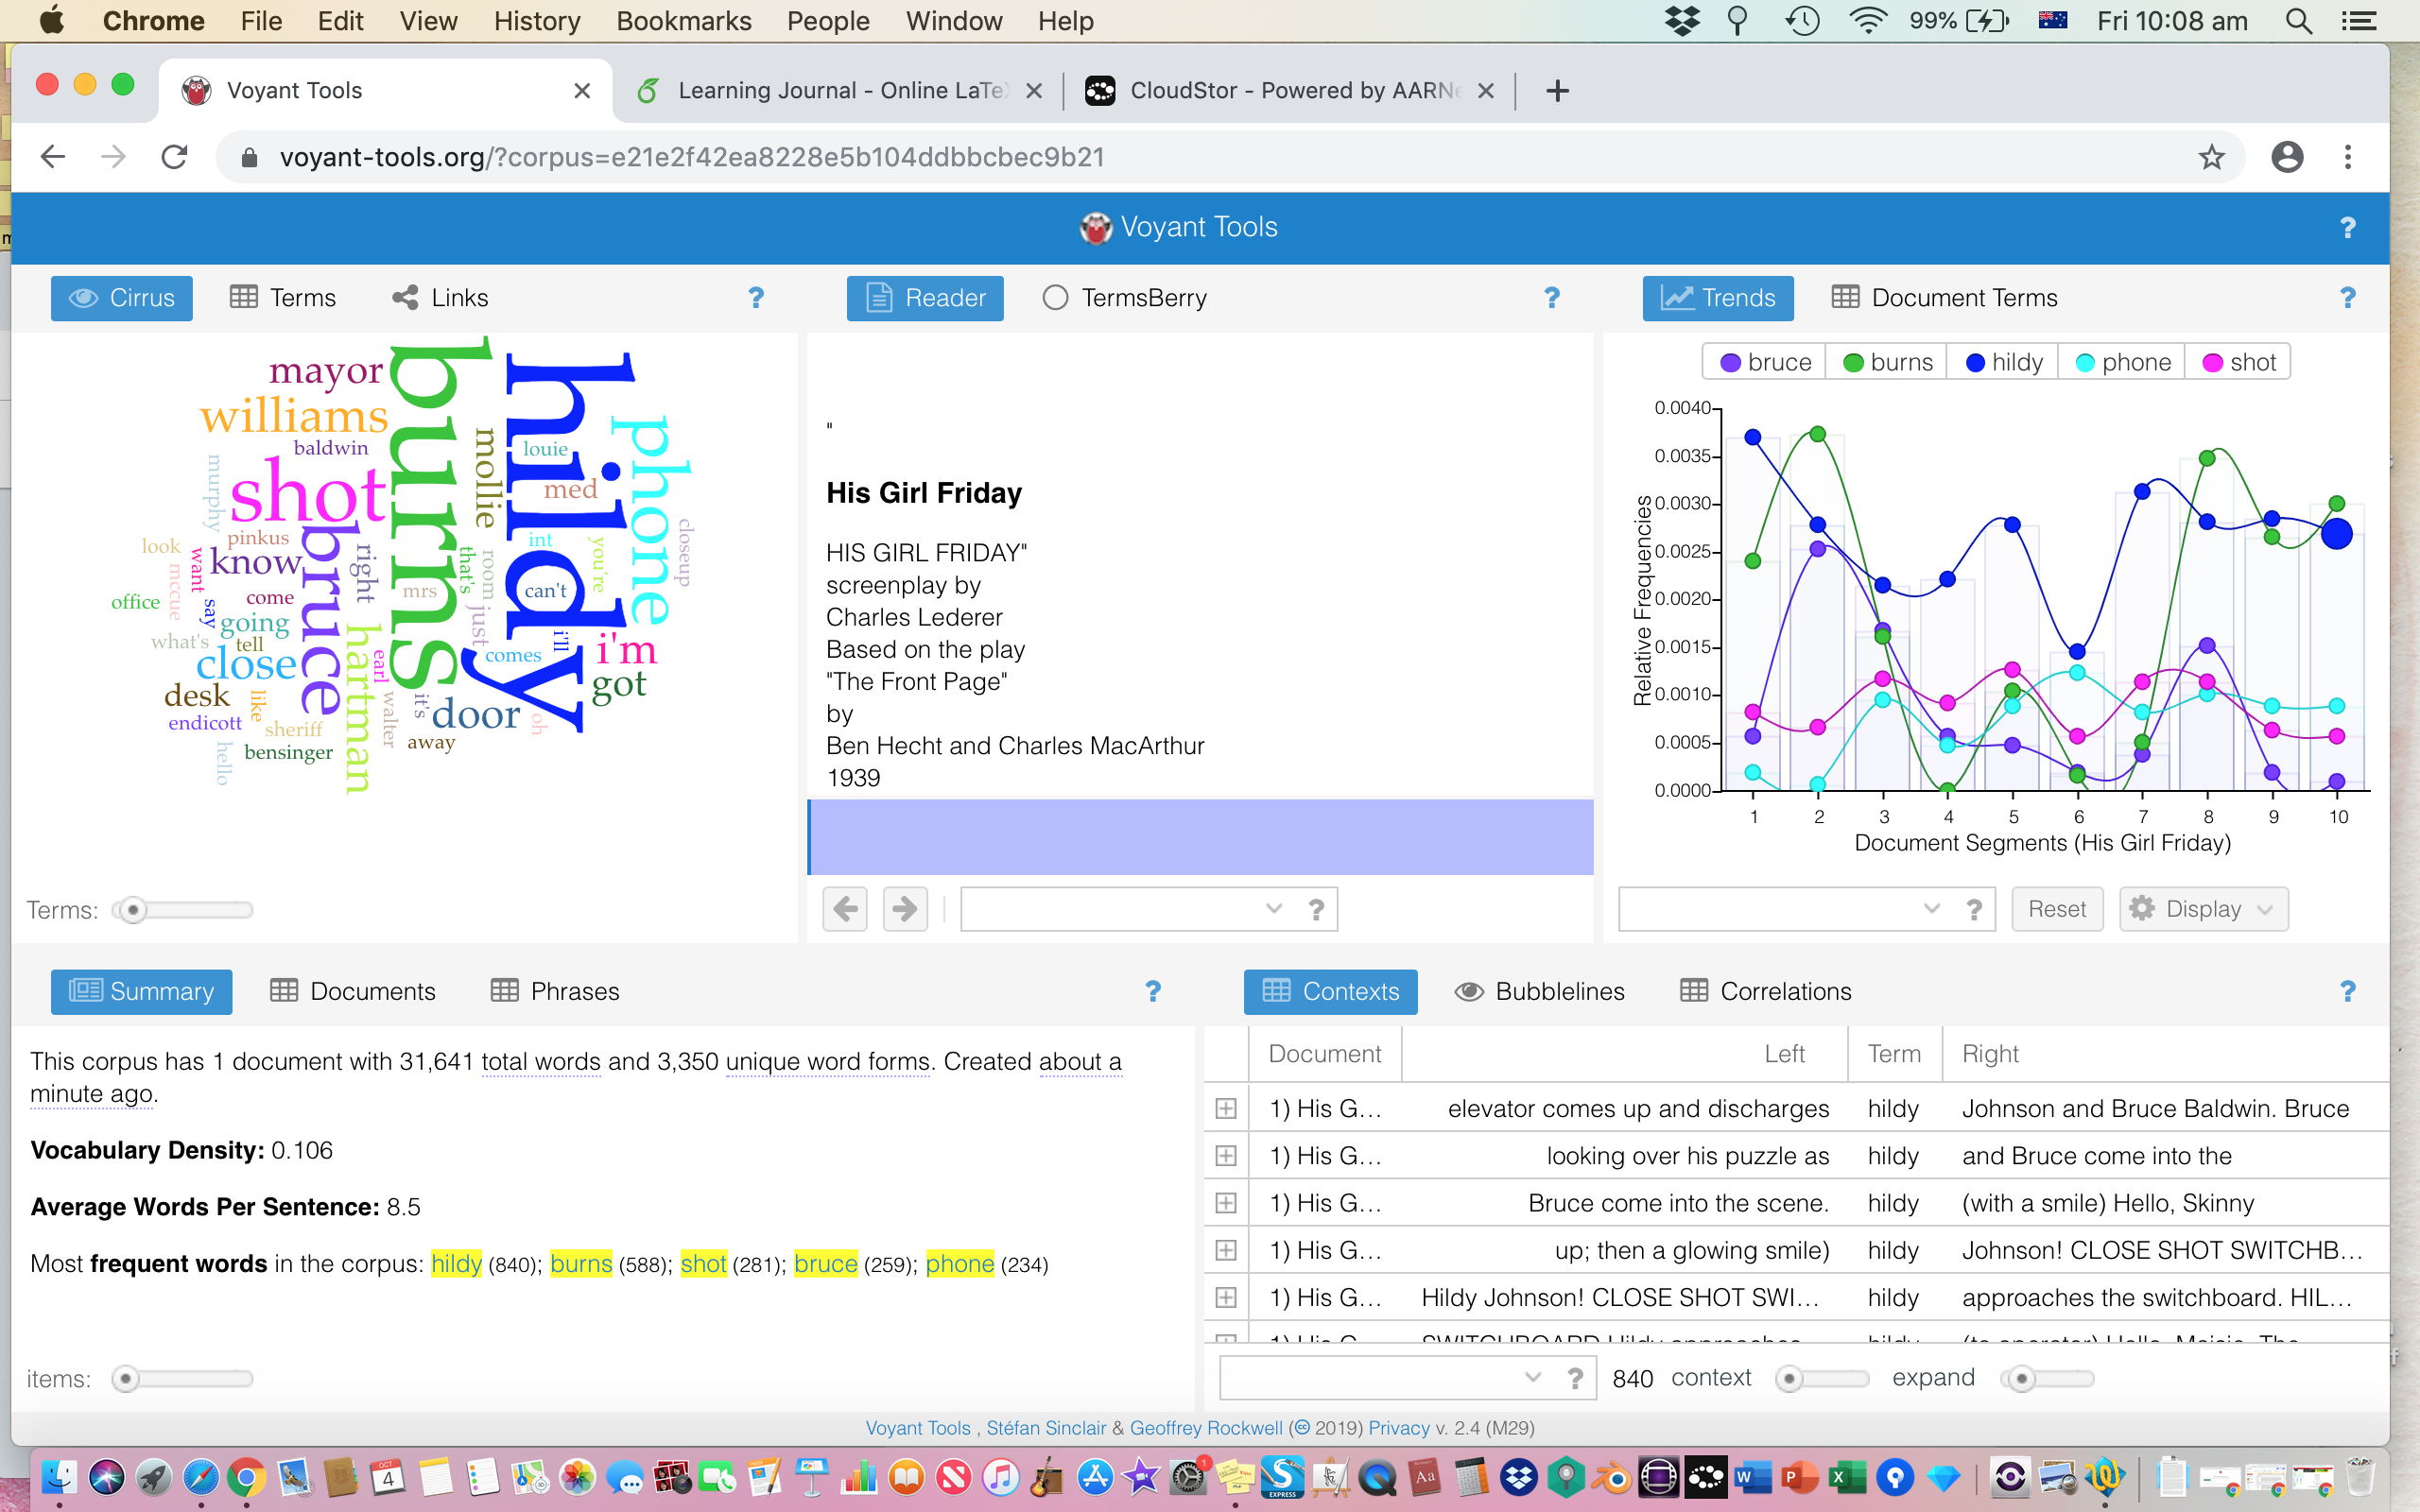
\includegraphics[width=10cm]{Voyant_Result.png}
    \caption{Result of Uploading \textit{His Girl Friday}(1940) Script to Voyant}
\end{figure}
\textbf{Errors:} None.\\
\textbf{Solutions/Notes:} My challenge now will be to determine how Voyant works and what each part of it is showing, and how I can adjust these.\\
\vspace{5mm}
\textcolor{blue}{Note: This is a really valuable source for how to use Voyant which I will use in completing future objectives} \url{https://voyant-tools.org/docs/#!/guide/tutorial}\\
\vspace{5mm}
\textbf{Objective: Exclude a Word From A Tool}\\ 
\textbf{Time Stamp:} 10:30am 4 October\\
\textbf{Actions:} I want to be able to omit a word from analysis by a tool (as well as all of the tools). I decided to work with the Cirrus tool. I hovered the mouse over the top of the Cirrus window. I then clicked on the icon to 'Define options for this tool'. In the options pop-up that appeared, I clicked on edit list. I added the word 'shot' to a new line as this word appeared quite frequently, but didn't really tell me anything about the script. I then clicked save. According to the guide having apply globally ticked should apply this to all the tools. I left apply globally ticked and then clicked the blue confirm button.\\
\textbf{Results:} This successfully removed 'shot' from Cirrus as well as the other tools (such as the summary and trends one)\\
\textbf{Errors:} None.\\
\textbf{Solutions/Notes:}\\
\vspace{5mm}
\textbf{Objective: Save a Corpus to Continue Working on Later}\\ 
\textbf{Time Stamp:} 10:38am 4 October\\
\textbf{Actions:} I went to the top right hand corner of the page, and clicked on the icon with the little box and arrow. I left selected, 'a URL for this view (tools and data)'. If I clicked the down arrow, there were also options for 'an HTML snippet embedding this view in another web page' or 'a bibliographic reference for this view'. I then clicked Export. This then opened the page I was viewing in another window. I copied this page's URL (\url{https://voyant-tools.org/?corpus=e21e2f42ea8228e5b104ddbbcbec9b21&stopList=keywords-651ab448fa5fefbff70938da9de39bfc&panels=cirrus,reader,trends,summary,contexts}\\
\textbf{Results:} When I pasted this link into a new Chrome window, it opened my corpus successfully. I can also export individual tools by going to the top right hand corner of the tool and following the same process outlined above.\\
\textbf{Errors:} None.\\
\textbf{Solutions/Notes:} Something I need to consider in the future is whether I need to re-export the link everytime I make changes (the answer to this is yes: I do, as I excluded a word for a tool and then re-entered the link above, and the change wasn't reflected).\\

\pagebreak

\subsection{oTranscribe}
This is a tool I plan to use in my proof of concept which allows you to transcribe notes while watching a video. While there is an online version, you can also download it from GitHub (\url{https://github.com/oTranscribe/oTranscribe}).
\vspace{5mm}
\textbf{Objective: Download The Repository From GitHub}\\ 
\textbf{Time Stamp:} 5:15pm 9 October\\
\textbf{Actions:} From GitHub I downloaded the current zip archive by clicking the link for this. I then unzipped the folder that downloaded and moved it to my Desktop.\\
\textbf{Results:} The contents of the repository downloaded successfully, as confirmed when I inspected the contents of the folder through GUI and compared it to GitHub.\\
\textbf{Errors:} None.\\
\textbf{Solutions/Notes:}\\
\vspace{5mm}
\textbf{Objective: Install node.js and npm}\\ 
\textbf{Time Stamp:} 6:05pm 9 October\\
\textbf{Actions:} I followed the link from the GitHub information to install node.js and npm, which took me to \url{https://nodejs.org/en/}. I selected the button, '10.16.3 LTS - Recommended for most Users', which began a download. I then opened the downloaded file and followed the prompts to install it.\\
\textbf{Results:} I received this message:\\
This package has installed:\\
Node.js v10.16.3 to /usr/local/bin/node\\
npm v6.9.0 to /usr/local/bin/npm \\
Make sure that /usr/local/bin is in your \$PATH.\\
\textbf{Errors:} None.\\
\textbf{Solutions/Notes:}\\
\vspace{5mm}
\textbf{Objective: Run npm install}\\ 
\textbf{Time Stamp:} 6:55pm 9 October\\
\textbf{Actions/Results:} In the terminal I entered 'npm install'. This created a file called package-lock.json in the /Users/Emily directory. However, reading the instructions again I think I was supposed to run this command from within the src folder in the downloaded repository folder. I first deleted the json file and then made the src folder the working directory in the terminal. I then ran 'npm install' again, and this printed a loading bar and then a lot of text. Looking through GUI, I believe this was successful as in the repository folder on my desktop a folder was created called node\textunderscore modules. The final line of the printed text in terminal was 'added 1107 packages from 1197 contributors and audited 7173 packages in 158.822s; found 742 vulnerabilities (232 low, 53 moderate, 454 high, 3 critical)'. I then ran 'npm audit fix'. This again printed a lot of text, with the final lines being '39 vulnerabilities required manual review and could not be updated; 7 package updates for 37 vulns involved breaking changes; (use `npm audit fix --force` to install breaking changes; or refer to `npm audit` for steps to fix these manually; run npm audit fix to fix them, or npm audit for details''. \\
\textbf{Errors:} None.\\
\textbf{Solutions/Notes:}\\
\vspace{5mm}
\textbf{Objective: Run build\textunderscore prod}\\ 
\textbf{Time Stamp:} 7:50pm 9 October\\
\textbf{Actions:} Still with the src folder as the working directory, I entered 'build\textunderscore prod \\
\textbf{Results:} See Errors\\
\textbf{Errors:} I received this message, 'make: *** No rule to make target `build\textunderscore prod'.  Stop.' I will go to consultation hours to get assistance in getting this to work.\\
\textbf{Solutions/Notes:} While waiting to speak to Brian at consultation hours before class, I tried running the command again, but with oTranscribe-master as a the working directory. This successfully created a 'dist' folder with a number of files included in it. The GitHub instructions say 'For a sourcemap and 'watch-for-changes', run make build\textunderscore dev', but I am yet to do this.\\
\vspace{5mm}
\textbf{Objective: Upload A Video File To The Online Version Of oTranscribe}\\ 
\textbf{Time Stamp:} 8:14pm 10 October\\
\textbf{Actions/Results/Errors:} I went to \url{https://otranscribe.com/} in Google Chrome and clicked on the Start transcribing button. I then selected the 'Choose audio (or video) file' button, and selected a .mov file on my computer (called Test.mov) which is a video I took of a parade. However, when I opened this file, I was advised it was unsupported and to either convert the file or use a different browser. I then followed this same process in Safari and the video file opened successfully which took me to a new page with the video in the top left hand corner of the page and a space to enter notes in the middle.\\
\textbf{Solutions/Notes:}\\
\vspace{5mm}
\textbf{Objective: Enter Notes In The Online Version Of oTranscribe}\\ 
\textbf{Time Stamp:} 8:32pm 10 October\\
\textbf{Actions:} At the page reached at the end of the previous objective, I selected a new line in the space to enter text (I left the notes already at the start of the document about quick tips there). I played and paused the video using the escape button (when resuming the video it rewinds the video a bit and doesn't start again exactly at the point it was stopped). To add a note, at the appropriate time, I pressed command and J at the same time, which inserted the timestamp on the line I was at in the space to type text. I added two notes, one at 01:27 (Start of the parade) and 01:44 (Start of the Australian Team). \\
\textbf{Results:} The notes were created successfully.\\
\textbf{Errors:} None.\\
\textbf{Solutions/Notes:} Other short cuts can be seen by clicking the cog in the top right hand corner of the page. A useful one is that I can press command and K to jump to the time in the video a note is referring to. The clip can be scrubbed through using the bar at the top of the page.\\
\vspace{5mm}
\textbf{Objective: Export Notes From The Online Version Of oTranscribe}\\ 
\textbf{Time Stamp:} 9:18pm 10 October\\
\textbf{Actions:} I selected the export icon on the right hand side of the page. This presents a menu allowing me to download the script in three different formats (Markdown(.md), Plain text(.txt) or oTranscribe format (.otr)) or send the transcript to Google Drive. I downloaded the transcript in each of the three different formats by selecting each one in turn, which automatically downloaded the file.\\
\textbf{Results:} The transcript exports were successful. Each file saved as 'Transcript exported Thu, 10 Oct 2019 10\textunderscore 20\textunderscore 06 GMT', with the appropriate file extension. I moved them all to a folder on my desktop called 'oTranscribe\textunderscore Tests'\\
\textbf{Errors:} None.\\
\textbf{Solutions/Notes:}\\
\vspace{5mm}
\textbf{Objective: Import Notes To The Online Version Of oTranscribe}\\ 
\textbf{Time Stamp:} 9:25pm 10 October\\
\textbf{Actions:} I went to \url{https://otranscribe.com/} in Safari, clicked on the Start transcribing button, and the notes I had written previously automatically appeared. I then opened Test.mov. However, I still wanted to try importing my notes, so I deleted the text that automatically appeared. I then went to the Import icon on the right hand side of the page, and navigated to the folder I had saved all my exported transcripts in. The only file type I was given the option to select was the .otr one, so I selected it and clicked Choose.\\
\textbf{Results:} My previous transcript was imported successfully.\\
\textbf{Errors:} None.\\
\textbf{Solutions/Notes:}\\
\vspace{5mm}
\textbf{Objective: Install Jekyll}\\ 
\textbf{Time Stamp:} 2:00pm to 5:00pm 11 October\\
\textbf{Actions/Results/Errors:} The next step of the GitHub instructions for downloading and running oTranscribe say to 'Upload the files in the newly-generated dist folder to a server of your choice'. In order to achieve this next step, Brian suggested in consultation hours that I install Jekyll. To do this, I followed each of the instructions (up until Global Install) at \url{https://jekyllrb.com/docs/installation/macos/}. These are just some notes on where I encountered extra actions that needed to be completed or any errors:
\begin{itemize}
    \item Entering 'xcode-select --install' printed the message 'xcode-select: error: command line tools are already installed, use "Software Update" to install updates'. I continued to the next instruction.
    \item When I ran the command to install Homebrew, I received a message about what folders would be created, and was asked to 'Press RETURN to continue or any other key to abort'. I pressed the return button, and then had to enter my computer password.
    \item The warning 'You don't have /Users/Emily/.gem/ruby/2.3.0/bin in your PATH, gem executables will not run' appeared after running a number of commands. I will need to check whether this creates an issue in the future.
    \item When I ran 'gem install --user-install bundler jekyll', it printed a lot of text which ended with 'ERROR:  Error installing jekyll:
	jekyll-sass-converter requires Ruby version >= 2.4.0.'. Brian informed me this was because I skipped the steps for Installing Ruby With rbenv (I assumed I had to follow the instructions for either Homebrew or rbenv, but I had to do both). I then went back and followed the instructions for rbenv.
    \item When I ran the command to check I had installed rbenv correctly, part of the text was in red, and said 'Checking for rbenv shims in PATH: not found'. It also said, 'Please run `rbenv init' and follow the instructions'. I ran 'rbenv init', and this printed, '\# Load rbenv automatically by appending; \# the following to ~/.bash\textunderscore profile:; eval "\$(rbenv init -)”'. I made the mistake of just entering the command 'eval "\$(rbenv init -)”', where I actually had to make a new file with this in it, which Brian helped me fix.
\end{itemize}
\textbf{Solutions/Notes:} Alternative instructions can be found at \url{https://github.com/rbenv/rbenv#homebrew-on-macos}.\\
\vspace{5mm}
\textbf{Resources:}\\ 
These are some resources suggested to me by Brian during consultation hours for completing future work:
\begin{itemize}
    \item Setting up a GitHub Pages site with Jekyll - \url{https://help.github.com/en/articles/setting-up-a-github-pages-site-with-jekyll}
    \item How to test my code does what I mean it to - \url{https://www.r-bloggers.com/unit-testing-with-r/}
    \item Combining Rcode with text \url{https://uomresearchit.github.io/r-tidyverse-intro/07-notebooks/}
    \item Also, make sure I write/save my code in an RNotebook.
\end{itemize}
\vspace{5mm}
\textbf{Objective: Set Up A GitHub Pages Site With Jekyll}\\ 
\textbf{Time Stamp: 11:00am 22 October} \\
\textbf{Actions/Results/Errors:} When reading the instructions at \url{https://help.github.com/en/articles/setting-up-a-github-pages-site-with-jekyll}, I was unsure about how to upload the dist folder I had compiled to the site so I sent a message to Brian on Slack. We then scheduled a video chat, as the process I needed to follow wouldn't be listed anywhere, and these are the actions I took as instructed by Brian.
\begin{itemize}
    \item Firstly, I went to my Hunt-Exercises repository on GitHub and clicked the green 'Clone or download' button, and then clicked the clipboard icon to copy the link to the repository.
    \item I then opened Terminal and made the Desktop my working directory. I then entered 'git clone' and pasted the link for the repository I had just copied and pressed Enter. This printed some text and created a Hunt-Exercises folder on my Desktop.
    \item I then entered in Terminal 'mkdir docs' which created a folder called 'docs' on my desktop.
    \item Through GUI I copied the contents of the dist folder into the new docs folder and then dragged and dropped the docs folder into the Hunt-Exercises folder.
    \item In terminal I entered 'git add -A'. While I wasn't sure at the time what this did, I looked it up and this command 'add(s) all new and changed files to the staging area' (\url{https://github.com/joshnh/Git-Commands})
    \item I then entered in Terminal 'git commit -am "Initial commit of folder for Git Pages”', and then 'git push' which committed the changes made to the Hunt-Exercises folder on my Desktop to the master in GitHub, with the commit message I had entered.
    \item I then went into the Hunt-Exercises repository on GitHub and went to the Settings Tab. I scrolled down to the GitHub Pages section. Under Source, I clicked the drop down menu and selected 'master branch/docs folder'. However, when the link this produced was clicked, the page said 'There isn’t a GitHub pages site here'.
    \item Brian said this was because GitHub was looking for a specific file and it couldn't find it, so he created it (file.md). Brian changed the site to run off the master branch rather than the 'branch/docs folder'.
    \item Going to the link now (\url{https://mq-foar705.github.io/Hunt-Exercises/}) successfully displayed a site, with a link to open oTranscribe which opened and functioned successfully.
    \item Brian said I could include my other documents on this static site. To edit it, I go to file.md. This information can help me with the formatting \url{https://mq-foar705.github.io/Hunt-Exercises/}
\end{itemize}
\textbf{Solutions/Notes:}\\
\vspace{5mm}

\pagebreak

\section{Errors}
\subsection{Overleaf}

\subsubsection{Useful Errors}
\autoref{sec:underfull} Underfull /hbox (badness ****) in paragraph at lines **\\
\autoref{sec:logcommand} Log Command Has Changed\\
\autoref{sec:description} Commit From Overleaf not Appearing in GitHub\\
\autoref{sec:space} No Space in Text Behind Special Characters

\subsubsection{Error: Overfull hbox (**pts too wide) in paragraph at lines **}
\textbf{Errors:} This error keeps appearing down the left hand side of the document where the lines are shown.\\
\textbf{Solutions/Notes:} I can find information on this from \url{https://www.Overleaf.com/learn/latex/Errors/Underfull_%5Chbox}
As this seems error seems to be indicating the text exceeds the margins of the page, I will try using \verb|\\| to put the text on a new line. 

\subsubsection{Error: Check that your \$'s match around math expressions. If they do, then you've probably used a symbol in normal text that needs to be in math mode. . .}
\textbf{Time Stamp:} 2:30pm 18 August\\
\textbf{Errors:} This kept appearing when I used an underscore in the text, and the error notification informed me that some symbols are used for mathematical calculations and have to be in math mode. I had previously just replaced underscores with dashes but wanted to address this issue.\\
\textbf{Solutions/Notes:} I used \verb|\textunderscore| to insert underscores where I needed them. However, when writing this journal entry where I had to include a dollar sign, I also discovered you can simply put a \verb|\| before the math symbol, or could use the same verb command I use when including code in the text.

\subsection{GitHub/Sourcetree}

\subsubsection{Useful Errors}
\autoref{sec:submodule} Submodule Not Visible in GitHub

\subsubsection{Error: Pushes from Overleaf Appearing in Connected Repository, but Not When it is Accessed Through Main Hunt-Exercises Repository}
\textbf{Time Stamp:} 10:00pm 16 August(Error)/10:00 am 18 August (Solution attempted)\\
Prior to attempting a solution, I asked advice from Brian on Slack.\\
\textbf{Actions:} Within Sourcetree, a Commit notification appeared. I clicked Commit, and within the description wrote, 'Commit changes from subdirectory into Hunt-Exercises', as well as the comment I put on the original push. I then clicked Commit. This then produced a one on the push symbol. I then completed the push and went into GitHub.\\
\textbf{Results:} This seemed to successfully make the changes appear in the repository.\\
\textbf{Notes:} I will now complete a new push with this added objective within the Overleaf file and follow these steps to see if it works. This worked successfully. Note however, prior to the first Commit notification appearing in Sourcetree, there is a Pull notification within the subdirectory that is being changed.

\subsection{Excel}
\subsubsection{Useful Errors}
\autoref{sec:cellformat} Cells in the Incorrect Format\\
\autoref{sec:formulacolumn} Cells Which Should Have a Formula Applied Not Automatically Populating\\
\autoref{sec:CSV} CSV Export Not Working\\

\subsection{The Unix Shell}
\subsubsection{Useful Errors}
\autoref{sec:help} Illegal Option/Getting Help\\

\subsubsection{Command Not Found}
\textbf{Time Stamp:} Numerous Occasions\\
\textbf{Action:} Check the spelling of the command. If this is not the issue, check online to see if the command is different.\\

\subsubsection{Error: Not Being Able to Move Up a Directory After Changing Working Directory (Using a Relative Path)}
\textbf{Time Stamp:} 3:20pm 25 August\\
\textbf{Actions:} I typed 'cd . .' and pressed enter. \\
\textbf{Results:} At first this didn't work and the response was 'command not found'. I then realised that there are not meant to be spaces between the dots and tried 'cd ..'. This worked and the prompt appeared with the parent (the directory containing) of the directory I had changed to the working directory. Also see Objective: Change the Working Directory Using an Absolute Path on page \pageref{absolute}\\
\textbf{Notes:} To be able to see the special directory (..) when running ls, type 'ls -F -a' (show all). In the response, the single dot is the current working directory. '.bash\textunderscore profile' is the file containing shell configuration settings and other files may have dots in front of them (see Navigating Files and Directories lesson for more details). To summarise .. means 'the directory above the current one' and . means 'the current directory'.

\subsubsection{Word Count Command Not Working}
\textbf{Time Stamp:} N/A\\
\textbf{Action:} As noted in the lesson, if you type 'wc' and click enter, you haven't added a file name so Terminal waits for you to provide input for it to process. To exit this, press control and 'c'.\\

\end{FlushLeft}


\end{document}
